\section{Protocol, and the amendments to it}
\label{app:protocol}

The corpus protocol is \protocolfile\ and the practice pilot's is
\pilotprotocolfile; both are in the archive and both were committed
before the first result they govern existed. This appendix lists what changed
afterwards.

\paragraph{Why amendments are reported rather than folded in}
A pre-registration that is quietly edited is worse than none, because it
claims a discipline it does not have. Each amendment below names the defect
that forced it and the result it moved; the protocol file in the archive
carries the date of every amendment.

\begin{description}
\item[Amendment 1 --- a register's values must recur across time.]
Registered rule 3.3 admits any attribute reused across two cases on average.
On BPI Challenge 2019 that admits the purchasing-document number, which is a
document identifier and not a maintained entity: almost none of its values
recur across the temporal split. The amendment adds a second, outcome-free
condition --- at least \minTrainCoverage\ of test cases must carry a value
seen in training --- and \emph{both} selections are reported for every log.

\item[Amendment 2 --- ``any timestamp'' had to be implemented.]
Rule 3.1 excludes timestamps. Matching a fixed list of names did not implement
that: it missed five differently-spelled date columns, two of which the
registered rules then made the high-cost entity. A column is now a timestamp
if its name looks like one or if more than $90\%$ of its non-missing values
parse as a date. Both tests read feature values only.

\item[Amendment 3 --- a relabelling of the activity is the activity.]
Some logs carry a second column that is a one-to-one recoding of
\texttt{concept:name}. Admitting it as a feature admits the activity sequence,
which is not available at case creation.

\item[Amendment 4 --- coarsenings of the register get their own role.]
Type, subtype and service are deterministic functions of the item. Sweeping
them into the intake block makes the intake block partly a register, and the
increment then measures the residual rather than the field. They are a
separate role and Section~\ref{app:layers} uses it.

\item[Amendment 5 --- the caused-by family is an outcome.]
A caused-by attribution is the output of diagnosis, not an intake observation.
Without this the registered rules made the caused-by configuration item the
high-cost entity on the flagship log.

\item[Amendment 6 --- the pilot frame's topical filter was nulled.]
The frame's keyword filter was applied to titles and abstracts, which is a
filter on how a paper describes itself rather than on what it does.
\texttt{results/s06\_frame.csv} reports what nulling it does to the estimates.
\end{description}

\paragraph{What the protocol fixed, before any of the results it governs}
The design space of Section~\ref{sec:surface}; the reference specification;
the exclusion of the intercept-only rung from every admissible set; the six
register-quality mechanisms and their levels; the five planned contrasts and
the Holm procedure --- fixed before this analysis round and not before the
data were seen, which is why Section~\ref{sec:planned} calls them planned
and not confirmatory; the two families over which simultaneous bands are
taken; and the two-stratum design of the practice pilot, including the
decision to adjudicate a sample of the papers the screen \emph{rejected}. The
commit that fixed them adds \specfixcommit\ and no result file.

\subsection{Related work, strand by strand}
\label{app:related}

Four further strands bear on the argument. \emph{Many-analysts studies} put
one question and one dataset to independent teams and observe the spread
directly \citep{silberzahn2018many,breznau2022observing}: they establish that
analytic variability is large without supplying an estimand for it, which is
what the surface is. \emph{Predictive multiplicity} and Rashomon sets study
near-equally accurate models that disagree on individuals
\citep{marx2020predictive,semenova2022existence} --- multiplicity at the level
of a fitted model, where this paper's is at the level of the design that
produced it. \emph{Benchmark-variance work in predictive process monitoring}
reports how far results move with the pipeline and the protocol
\citep{ramamaneiro2021deep}, which is the evidence this paper's decomposition
partitions. And the \emph{sensitivity-analysis} tradition of bounding an
unmeasured assumption \citep{vanderweele2017sensitivity} is the form
Section~\ref{sec:quality}'s leakage tipping point takes. On the estate side,
the accuracy of a configuration management database is itself a studied
quantity \citep{suriadi2017imperfection,mohammed2025dataquality}, and the
layered service models practitioners maintain are why
Section~\ref{app:programmeread} asks which \emph{layer} of a register pays.
The strands are set out below, each with what this paper takes
from it.


%%  ROUND TWENTY-FIVE.  Moved from Section 2 for length, unchanged.

\paragraph{Variable importance and incremental value}
That a feature's apparent importance depends on what else is in the model is
the standard motivation for conditional and permutation-based importance
\citep{strobl2008conditional,fisher2019models}, for Shapley-value attributions
\citep{lundberg2017unified,covert2020sage}, and for nonparametric formulations
of importance as a population quantity \citep{williamson2021vimp}, which
average over subsets precisely because a single conditioning set is arbitrary.
The clinical-prediction literature has made the same point about the
\emph{incremental} value of a marker for two decades: the increase in the area
under the ROC curve from adding a predictor depends on how good the existing
model is \citep{pencina2008evaluating,cook2007roc}, is a poor guide to
clinical usefulness \citep{cook2007roc,vickers2008decision}, and is routinely
misread \citep{kerr2011evaluating}. What that literature establishes, and what
we take as given, is that the baseline and the metric are choices. What it
does not supply is an object that reports the whole dependence, an estimator
for it, or inference over it.

\paragraph{Decision-analytic evaluation}
Decision curve analysis \citep{vickers2006dca,vickers2016net} makes the
operating point explicit by reading net benefit across an exchange rate, and
is the reason the operating point is an axis here rather than a footnote.
Guidance on reading such a curve is well developed \citep{vickers2019simple};
what is less settled is what a claim about a \emph{band} of thresholds
requires, which is why the bands in Section~\ref{sec:dca} are simultaneous
rather than pointwise.

\paragraph{Specification sensitivity}
That analytic conclusions move with defensible analytic choices is the subject
of multiverse analysis \citep{steegen2016increasing}, specification-curve
analysis \citep{simonsohn2020specification}, vibration of effects
\citep{patel2015assessment} and, in machine learning evaluation, of work on
underspecification \citep{damour2022underspecification} and on the fragility
of benchmark rankings \citep{bouthillier2021variance}. Our design space and
our figures are recognisably in that tradition. What this paper adds to it is
a decomposition of the surface's variance into axis contributions,
simultaneous inference over the surface rather than a distribution of point
estimates, region labels with an explicit decision rule, and a regret
benchmark against the conventional report. Specification-curve analysis, as
usually practised, displays the curve and applies a permutation test to its
median; it does not tell a reader which sub-region of the design space
supports a sign.

\paragraph{Data valuation}
Shapley-based data valuation \citep{ghorbani2019data,jia2019towards} values
\emph{instances} against a fixed learner and metric; the axes we vary are
exactly the ones held fixed there. The two are complementary: a data value is
itself a point on a specification surface.

\paragraph{Which axis a study varies}
Some studies do vary one axis deliberately: the metric axis in effort-aware
defect prediction \citep{carka2022effortaware}, the encoding axis in
remaining-time prediction \citep{liu2025encoding}, the inter-case feature
block in predictive process monitoring \citep{senderovich2017intercase}. What
is missing is an object that holds several axes at once and says what their
joint variation implies for a sign.

\paragraph{Prediction on incident event logs}
The empirical setting is predictive process monitoring, surveyed and
benchmarked across real logs
\citep{teinemaa2019outcome,verenich2019survey} on data of the kind process
mining formalises \citep{vanderaalst2016process}. We predict at case creation
from creation-time attributes with no prefix, which is tabular classification
on a process log rather than prefix-based monitoring, and that difference
bounds what the corpus result transfers to. The benchmark protocols in that
literature fix a learner, an encoding and a metric per experiment, and this
paper measures the sensitivity of a conclusion to \emph{those} fixings. It
does not measure sensitivity to \textbf{prefix length, prefix bucketing or
sequence encoding}, which are the axes that literature varies most, because
none of them exists at a single prediction point; Section~\ref{sec:lim}
carries the transfer as an assumption rather than a result. Configuration
management databases and their data quality are treated in the IT service
management literature as an operational problem \citep{marrone2011itil}; we
are not aware of an evaluation of one against a named prediction task with the
design space held open.

\paragraph{Data quality as an axis}
The effect of data quality on model performance has been studied directly on
tabular data \citep{mohammed2025dataquality} and, in process mining, for
low-quality activity labels \citep{comuzzi2025labels}. Those studies vary
quality with the feature set fixed; we vary quality \emph{as one axis of the
same surface} on which the feature set and the encoding are others, which is
what makes the interaction between them visible ---
Section~\ref{sec:quality} reports a quality defect that is exactly invisible
under one encoder and not under another. Leakage, which is availability
misspecified, has its own literature
\citep{kaufman2012leakage,kapoor2023leakage,weytjens2022leakage}, and the
forecast origin of Section~\ref{sec:twodecision} makes it a declared choice
rather than a mistake.

\subsection{The measure on the axes, and the two axes that are not analysis choices}
\label{app:measurechoice}

%%  ROUND TWENTY-FIVE.  Moved from the article for length, unchanged.

\paragraph{On the measure}
A design space is a set; a decomposition, a weighted mean or a robustness
index needs a \emph{distribution} on it, and ``uniform over the cells I
enumerated'' is not neutral --- it moves if a level is duplicated, if five
folds are written as five levels rather than one, or if a grid is refined.
This paper separates the weight on an axis from the weights within it,
declares three product measures and an envelope over a fourth
(Section~\ref{sec:sobol}), and reports every weighted quantity under all of
them.

Two of these axes deserve comment because they are usually not treated as
design choices at all.

The \textbf{forecast origin} $\tau$ fixes which fields exist when the prediction
is made. It is not the same as the split rule and it is not a data-cleaning
detail: moving $\tau$ later in a process admits fields written in between, and
Section~\ref{sec:cmdb} is a case in which that single move takes a field's
increment from resolvably positive to indistinguishable from zero.

The \textbf{register quality} $q$ acts on $f$ rather than on the comparison. A
field that is a lookup into a maintained register --- a configuration item, a
customer master record, a product catalogue --- inherits that register's
completeness and accuracy. We implement \nQualityKinds\ mechanisms besides the
clean field, each parameterised by the training half alone: population loss
with the long tail absent, with the core absent, and at random; identity
error, in which a share of rows carry a wrong value drawn from the training
alphabet; reconciliation failure, in which a share of identities exist twice;
and staleness, in which an identity is present only if the register had
already seen it by the split point. The first three model coverage, the next
two accuracy, the last discovery; the taxonomy follows the event-log
imperfection patterns of \citet{suriadi2017imperfection} where they apply.

Real registers do not fail at random, so three \emph{further} mechanisms make
the missingness depend on something: on \emph{time}, where a row's probability
of carrying an identity rises with its position in the log; on \emph{content},
where coverage depends on the item's recorded type through a map estimated on
the training half; and on a \emph{propensity} built from the intake block,
which makes missingness correlated with the outcome without ever reading a
test outcome. Every mechanism is swept over \nQualityLevels\ severities and
every stochastic one repeated over \nQualitySeeds\ seeds, and each is verified
by execution to be a function of the training half alone --- perturbing the
test half and re-degrading must leave the training half's degraded values
identical, which \texttt{results/s01\_trainonly.csv} records over \nTrainOnly\
checks.

\subsection{Targets, splits and the exclusion codes}
\label{app:targets}

%%  ROUND TWENTY-FIVE.  Moved from the article for length, unchanged.

Two targets are defined for every log: \emph{handover}, whether more than one
resource group touches the case, and \emph{duration}, whether the case runs
longer than the training half's median. Cases are ordered by their first
timestamp and split $70/30$; the rolling-origin scheme adds \nFolds\
expanding-window folds. Fields that are determined only at closure are excluded by name, which is the
standard leakage discipline \citep{kaufman2012leakage,kapoor2023leakage} and,
for event logs specifically, the discipline of
\citet{weytjens2022leakage}. A log--target pair is excluded only for a
registered reason --- too few cases, no variation in the test half, a prevalence outside
$[\prevLo, \prevHi]$, or the absence of one of the three roles --- and every
exclusion is reported with its code in Table~\ref{tab:corpus}, which accounts
for every downloaded log that is not among the admitted pairs --- including
the held-out set, \nHeldOutLogs\ of the checksummed files, downloaded for a
separate test and never offered to these rules at all.


\textbf{Every admitted pair is analysed and reported.} Running the full
surface only on the logs whose \emph{reduction} is resolvable would condition
the analysis on the outcome. The surface is computed on all \nPairs\ admitted
pairs through one code path, and the pairs on which the register is worth
nothing are in the same tables as the rest.

\subsection{The admission margin at the upper edge}
\label{app:margin}

%%  ROUND TWENTY-FIVE.  Moved from the article for length, unchanged.

\paragraph{The pair carrying the most cells sits closest to the admission
edge} \logAdmittedMaxPrev\ has the highest prevalence of any admitted pair,
\prevAdmittedMax, against the window's upper bound of \prevHi; the nearest
pair the headroom rule turns away, \logExcludedAboveMin, is at
\prevExcludedAboveMin, and \nExcludedAbove\ pairs in all are excluded above
the bound. That pair is also the largest single contributor to the corpus,
carrying \nCellsLargestPair\ of the \nComputationalCells\ admissible scalar
cells. A rule with a sharp edge decides some case narrowly, and this is that
case: the corpus's biggest component is admitted on a margin narrower than
the gap to the pairs excluded beside it. Table~\ref{tab:family} reports every
headline statistic on the ITSM-like subset as well, which is the population
that does not turn on this decision.



\section{Proof details and constructions}
\label{app:props}
\begin{remark}[What survives a declared family of recalibrations]
\label{prop:rank}
For a family $\Psi$ of strictly increasing maps applied simultaneously to all
four arms of a configuration, the reduction is $\Psi$-invariant exactly when
the metric is \emph{affine} under $\Psi$. Rank-basedness is sufficient and not
necessary, and the gap is family-relative: the class-mean gap --- the
difference in mean score between the two outcome classes, which is not
rank-based --- has a reduction invariant to \widerRShiftAffine\ inside the
affine family and shifting by up to \widerRShiftNonAffine\ over
\nPsiFamiliesNonAffine\ non-affine ones. What this buys is that a search
becomes a proof: one map and one configuration violating the invariance rules
it out everywhere, and \nCertificates\ such certificates are computed, the
smallest moving the reduction by \certificateMinShift, against
\nInvarianceChecks\ checks in which the two rank-based metrics hold to
\invarianceMaxShift.
\end{remark}

\subsection*{Remark~\ref{prop:nonid}: the two-point algebra in full}

Let a scoring rule take one of two values, with $a$ of the $P$ positives and
$b$ of the $N$ negatives in the high block; write $\alpha = a/P$,
$\beta = b/N$, $\rho = N/P$ and $\pi = P/(P+N) = 1/(1+\rho)$. Two exact
identities follow directly from the definitions of the two metrics
(Section~\ref{sec:surface} of the article):
\[
\mathrm{AUC} = \tfrac12 + \tfrac{\alpha - \beta}{2},
\qquad
\mathrm{AP} = \alpha\,\frac{\alpha}{\alpha + \beta\rho} + (1-\alpha)\pi .
\]
The first is the Mann--Whitney statistic with ties at $1/2$; the second is the
step-wise sum over the two operating points the rule admits. Hence
\[
\mathrm{AP} - \pi \;=\; \alpha\left(\frac{\alpha}{\alpha + \beta\rho} -
\pi\right).
\]

Fix $d = \alpha - \beta > 0$. Every rule on the line $\beta = \alpha - d$ has
the same AUC increment $d/2$ over the fully tied baseline, so any two of them
give $R_{\mathrm{AUC}} = 0$ exactly. Along that line the AP increment runs
from $d(1-\pi)$ at $\alpha = d$, $\beta = 0$ down to
$\dfrac{d\rho}{\bigl(1 + (1-d)\rho\bigr)(1+\rho)}$ at $\alpha = 1$, a ratio of
about $1 + \rho$. How far apart the two reductions can be pushed therefore
grows with the imbalance, which is a property of the construction and not a
hidden assumption: refuting the existence of $\varphi$ needs only that the two
be \emph{different}, and at the modest $\rho = \propOneRho$ this paper uses
they differ by \propOneApGap.

\subsection*{Remark~\ref{prop:rank}: the cancelling configuration, and
what a certificate is}

This section notes a configuration on which a non-rank-based
metric's increment moves under $\psi$ while the ratio does not. The
construction is immediate once stated: take $\sigma_{B_1} = \sigma_{B_0}$ and
$\sigma_{B_1 \cup f} = \sigma_{B_0 \cup f}$. Then $V(B_1) = V(B_0)$ for every
metric and every $\psi$, so $R = 0$ identically, while $V$ itself moves under
$\psi$ whenever $m$ is not rank-based. The configuration is degenerate --- the
two baselines induce the same scores --- and that is why the remark
quantifies over configurations rather than asserting a
configuration-by-configuration change.

A \emph{certificate} for a metric $m$ and a recalibration $\psi$ is a
triple of score vectors $(a,b,c)$ on one labelled test set for which
\[
\frac{m(b) - m(a)}{m(c) - m(a)}
\;\neq\;
\frac{m(\psi b) - m(\psi a)}{m(\psi c) - m(\psi a)} .
\]
By Remark~\ref{prop:rank} the existence of one such triple establishes
that $\psi$ does not act affinely on $m$, and therefore that $R_m$ is not
invariant --- a conclusion about \emph{every} configuration drawn from a
finite object. The certificates are searched for by maximising the gap over
random triples; \texttt{results/s29\_certificates.csv} records, for every
metric and every recalibration family, the triple found, the two ratios,
and the resulting shift in $R$. The search reports failure where it fails, and
a failure is not evidence of invariance.

\subsection*{Remark~\ref{prop:nonid}: the construction}

\begin{proof}[Proof (construction)]
Take $P$ positives and $N$ negatives and let every score take one of two
values, so a scoring rule is described by the pair $(a,b)$ counting positives
and negatives in the high block; write $\alpha = a/P$, $\beta = b/N$,
$\rho = N/P$. Both baselines are the fully tied rule $\alpha = \beta = 1$,
which has $\mathrm{AUC} = 1/2$ and $\mathrm{AP} = \pi$, the prevalence. Then
exactly
\[
\mathrm{AUC} - \tfrac12 = \tfrac{\alpha - \beta}{2},
\qquad
\mathrm{AP} - \pi = \alpha\left(\frac{\alpha}{\alpha + \beta\rho} - \pi\right).
\]
Fixing $\alpha - \beta$ equal on the two legs makes the AUC increments equal,
hence $R_{\mathrm{AUC}} = 0$ exactly --- in integers, not to rounding ---
while sliding $\alpha$ along the admissible range moves the AP increments and
sweeps $R_{\mathrm{AP}}$. With $P = \nPropP$, $N = \nPropN$ and therefore
$\rho = \propOneRho$, the two configurations in
\texttt{results/s29\_prop1.csv} --- $(\alpha,\beta)$ of $(0.8, 0.4)$ and
$(0.6, 0.2)$ in one, $(0.9, 0.5)$ and $(0.5, 0.1)$ in the other --- have
identical $R_{\mathrm{AUC}}$ to \propOneAucGap\ and $R_{\mathrm{AP}}$ of
\propOneRapA\ against \propOneRapB, differing by \propOneApGap. A single
$\varphi$ cannot take one input to two outputs.

The construction is only a proof if those two conditions hold, so
\texttt{s29\_props.py} asserts both: it refuses to write its output if the two
configurations fail to share $R_{\mathrm{AUC}}$ or fail to separate
$R_{\mathrm{AP}}$. A far more imbalanced problem, such as $\rho = 500$, drives the
gap close to one, and the modest
$\rho$ here shows the separation does not depend on extreme imbalance.
\end{proof}

\subsection*{Remark~\ref{prop:rank}: the proof}

The equivalence's harder direction needs one assumption.

\begin{assumption}[Richness]
\label{ass:rich}
Every quadruple of score vectors on the fixed labelled test set is realisable
as a configuration. This is the assumption that no restriction is placed on
the model class; it is what makes ``for every configuration'' quantify over a
set with more than three elements, and it fails only if the analyst commits in
advance to a family of scoring rules narrow enough to constrain the four arms
jointly. It is used only for (i) $\Rightarrow$ (ii); the direction that
matters in practice needs none.
\end{assumption}

\begin{proof}
(ii) $\Rightarrow$ (i). Each of $V_m(B_0)$ and $V_m(B_1)$ is a difference of
two values of $m$, so an affine change of scale multiplies both by $A(\psi)$
and the additive constant cancels; their ratio, and hence $R_m$, is unchanged
wherever the denominator is nonzero.

(i) $\Rightarrow$ (ii). Fix $\psi$ and the test set, and write $m(\sigma)$ for
$m(\sigma,y)$. For score vectors $a, b, c$, Assumption~\ref{ass:rich} admits
the configuration
$\sigma_{B_0} = a$, $\sigma_{B_0 \cup f} = c$, $\sigma_{B_1} = a$,
$\sigma_{B_1 \cup f} = b$, for which
$R_m = 1 - \bigl(m(b) - m(a)\bigr)/\bigl(m(c) - m(a)\bigr)$. Invariance says
\begin{equation}
\label{eq:ratiopres}
\frac{m(b) - m(a)}{m(c) - m(a)}
\;=\;
\frac{m(\psi b) - m(\psi a)}{m(\psi c) - m(\psi a)}
\end{equation}
for every admissible triple. First, the map $T : m(\sigma) \mapsto
m(\psi\sigma)$ is well defined: if $m(b) = m(b')$ then applying
\eqref{eq:ratiopres} to $(a,b,c)$ and to $(a,b',c)$ with the same $a,c$ gives
$m(\psi b) = m(\psi b')$. Second, fix $a$ and $c$ and put
$k = \bigl(T(m(c)) - T(m(a))\bigr)/\bigl(m(c) - m(a)\bigr)$; then
\eqref{eq:ratiopres} reads $T(u) = T(m(a)) + k\,(u - m(a))$ for every
$u$ in the range of $m$, which is affine with slope $A(\psi) = k$ and
intercept $B(\psi) = T(m(a)) - k\,m(a)$. The slope is nonzero because
otherwise the transformed denominator vanishes and $R_m$ is undefined rather
than invariant.
\end{proof}

\subsection*{Proposition~\ref{prop:scale}: the $3\times 3$ construction}

\begin{proof}[Proof (construction)]
Two levels per axis will not do, and the reason is worth stating: with two
levels the two main effects are $|P+Q|$ and $|P-Q|$, where $P$ and $Q$ are the
two within-axis differences, so their ordering is decided by
$\operatorname{sign}(PQ)$, and a strictly increasing $\phi$ preserves the sign
of each difference. At two levels the ordering is therefore \emph{invariant}
and the proposition is false. From three levels a conditional mean averages
more than two cells and a convex $\phi$ reweights them unequally. The
$3 \times 3$ design in \texttt{results/s07\_prop3.csv} has
$S_A = \pThreeRawA$ against $S_B = \pThreeRawB$ in its own units and
$S_A = \pThreeSqrtA$ against $S_B = \pThreeSqrtB$ under $\phi = \sqrt{\cdot}$,
so the leader changes.
\end{proof}

\subsection*{Why the second remark is stated relative to a family}

%%  ROUND TWENTY-FIVE.  Moved here from Section 3.5 for length.

It is stated \emph{relative to a declared family of recalibrations}, which is
both what its proof reaches and what an analyst can act on: nobody
recalibrates by an arbitrary monotone map, and a reader who has declared
that they will consider Platt scaling, or isotonic regression, or any affine
rescaling, is asking about that family and not about all of them.

Richness is used only in the direction (i) $\Rightarrow$ (ii), so under a
model class too narrow to realise the separating configuration a metric
can be invariant on \emph{that class} without acting affinely; the direction
that matters for practice, (ii) $\Rightarrow$ (i), needs no richness at all.
A reader working inside a restricted family should read the remark as a
sufficient condition and establish non-invariance on their own class by
exhibiting a configuration in it, which is what the certificates do.


\section{Construction of the inferential objects}
\label{app:objects}

Section~\ref{sec:inference} states what each of the reporting objects is and
why it is that and not something else. This appendix carries the constructions
themselves, so that the section can be read for the argument and this one for
the arithmetic. What is here is the detail a reader would need to reimplement
the objects without reading the code.

\subsection*{The multiplier bootstrap for the max-$t$ critical value}
\label{app:multiplier}

Let $\mathcal{F}$ be the declared family, $V^{(b)}_c$ the $b$th bootstrap draw
at cell $c$, $\bar V_c$ the draw mean and $\hat\sigma_c$ the per-cell
bootstrap standard error. Standardise the draw matrix,
\[
Z_{b,c} \;=\; \frac{V^{(b)}_c - \bar V_c}{\hat\sigma_c},
\qquad b = 1,\dots,B, \quad c \in \mathcal{F},
\]
and let $e_1,\dots,e_B$ be independent standard normals drawn afresh for each
replicate. The \emph{multiplier} statistic is
\[
T^{(\mathrm{mult})} \;=\; \max_{c \in \mathcal{F}}
\Bigl| B^{-1/2}\textstyle\sum_{b} e_b Z_{b,c} \Bigr| .
\]
Conditionally on the draws, $B^{-1/2}\sum_b e_b Z_{b,\cdot}$ is a centred
Gaussian vector whose covariance is exactly the empirical covariance of the
standardised draws, so the distribution of $T^{(\mathrm{mult})}$ approximates
that of the max-$t$ statistic without any further refitting
\citep{chernozhukov2013gaussian}. The critical value $q_{1-\alpha}$ is the
$(1-\alpha)$ quantile of \nMultiplier\ such replicates, generated in chunks so
that the ${\nMultiplier}\times B$ normal matrix is never held at once.

Two properties are worth stating because they are the reason the construction
is used here. The precision of $q$ is governed by the number of multiplier
replicates and not by $B$, so a design whose fitting budget is fixed by the
cost of refitting an entire pipeline can still resolve its critical value; and
because the multiplier draws are conditional on the observed $Z$, the
construction inherits whatever dependence the moving-block resampling induced
across cells, which is what a family-wise statement over a correlated surface
requires. The approximation is asymptotic in the same sense the max-$t$ band
is: it needs the high-dimensional central limit theorem to hold over a family
whose size is comparable to the draw count, which Section~\ref{app:threats}
states as an assumption rather than a guarantee.

The Monte Carlo interval for $q$ itself is retained. Writing
$[q^-, q^+]$ for the order-statistic interval of the multiplier quantile, a
cell is called \emph{resolved} only if its band excludes zero at $q^+$, so
residual Monte Carlo noise leaves cells unresolved rather than resolving them
in the wrong direction.

\subsection*{Fieller's construction for the reduction}
\label{app:fieller}

For $\vartheta = V_1 / V_0$ with estimates $(\hat v_0, \hat v_1)$ and
bootstrap covariance $(\hat s_{00}, \hat s_{11}, \hat s_{01})$, Fieller's
theorem gives the confidence set
\[
\Bigl\{\vartheta : (\hat v_1 - \vartheta \hat v_0)^2 \leq
z^2\bigl(\hat s_{11} - 2\vartheta \hat s_{01} +
\vartheta^2 \hat s_{00}\bigr)\Bigr\},
\]
whose boundary solves a quadratic in $\vartheta$ with leading coefficient
$\hat v_0^2 - z^2 \hat s_{00}$. When that coefficient is positive the set is a
bounded interval. When it is zero or negative --- which is exactly the case in
which the denominator $\hat v_0$ is not resolvably different from zero at
level $z$ --- the set is a half-line, the whole line, or the complement of an
interval, and reporting a bounded interval for it is reporting a set that is
not the confidence set. \texttt{results/s02\_fieller.csv} records the kind of
every set this paper computes, in its \texttt{fieller\_kind} column.

\paragraph{The three rules for the reduction} The article makes $D$ and the two increments primary and treats $R$ as a secondary descriptive statistic subject to three rules, declared before any $R$ was computed:
\begin{enumerate}
\item $R$ is reported only where $V_s(f \mid B_0)$ is resolvably positive
under the \emph{simultaneous} band, not merely positive as a point estimate;
\item its interval is a Fieller set and its \emph{kind} --- bounded,
unbounded, or the complement of an interval --- is printed beside it. A
confidence set for a ratio is the solution set of a quadratic
\citep{fieller1954} and is bounded only when the denominator is resolvably
away from zero (Section~\ref{app:fieller}). Of the \nFieller\ reductions this paper
computes, \nFiellerUnbounded\ have a non-bounded Fieller set, and a percentile
interval reports a bounded one for every single one of them;
\item the magnitude of $R$ is never compared with the spread of $R$ across
metrics as though both lived on an unproblematic common scale.
\end{enumerate}

\subsection*{The three regret designs}
\label{app:regretdesigns}

Section~\ref{app:regretfull} defines the sign-disagreement rate $M(s)$ and the regret
$G(s)$ and explains why an average of $G$ taken across metrics has no
units. The three designs it names are constructed as follows.

\begin{description}
\item[A. Metric-specific.] For each scalar metric $m$ separately, the
admissible set is restricted to the cells whose metric axis is at $m$, and
$M(s)$ and $G(s)$ are computed over that restriction under the declared
measure. Every reported value carries the name of its unit, and no average is
taken across metrics. The only cross-metric statement the design
permits is a count: in how many of the five metrics the \emph{direction}
of a conclusion is the same, and which ones it is not --- and
Section~\ref{sec:rules} reports both, because on this corpus two of those
counts are four and not five. The design assumes nothing beyond the measure,
and it is what the headline uses.

\item[B. Common operational utility.] Net benefit at threshold $t$,
\[
\mathrm{NB}(t) \;=\; \frac{\mathrm{TP}(t)}{n}
\;-\; \frac{\mathrm{FP}(t)}{n}\cdot\frac{t}{1-t},
\]
is measured in true positives per case at an exchange rate the threshold
declares, so values at different thresholds are cardinally comparable and may
be averaged. The increment is the difference in net benefit between the two
arms at the same threshold, computed only on calibrated probabilities
(Section~\ref{sec:dca}) because a threshold read as a cost ratio requires one.
The resulting quantity is called \emph{decision} regret rather than
predictive-performance regret. The design assumes a distribution over
thresholds, which is declared and varied rather than fixed.

\item[C. Partial identification.] If a reader insists on one number across
metrics, the answer depends on a map $\phi$ from a metric's units to
theirs. Five are declared, in
\texttt{s23\_regret.UTILITY\_MAPS}: the \emph{identity}; division by the
metric's remaining \emph{headroom}, the distance left to a perfect score;
division by the increment's \emph{standard deviation} across the surface; a
signed \emph{square root}; and a logistic squashing of the standardised
increment. Each is increasing in the increment and each divides only by
positive quantities, so all five fix zero and the \emph{sign} of an increment
is invariant to every one of them; what moves is the relative magnitude an
metric contributes to a mixed average. The conclusion is reported as its
\emph{range} over the family together with the part invariant to all of it,
which is exactly the part the design declines to identify.
\end{description}

Designs A and C are computed on the full declared surface, since neither needs
a bootstrap draw. Design B is computed on the calibrated decision-curve cells
of Section~\ref{sec:dca}.

\subsection*{Estimating the decomposition}
\label{app:sobolest}

Write $\mathbb{P} = \bigotimes_i w_i$ for the product measure over the axes.
Every subset $u$ of axes has a component $g_u$ given by the M\"obius sum over
the conditional means,
\[
g_u(x_u) \;=\; \sum_{v \subseteq u} (-1)^{|u| - |v|}\,
\mathbb{E}_{\mathbb{P}}\!\left[V \mid x_v\right],
\qquad
D_u \;=\; \mathbb{E}_{\mathbb{P}}\!\left[g_u^2\right],
\]
and the components are mutually orthogonal, so
$\sum_{u \neq \emptyset} D_u = \operatorname{Var}(V)$ exactly. The first-order
and total indices of Section~\ref{sec:sobol} are $S_i = S_{\{i\}}$ and
$S_{T_i} = \sum_{u \ni i} S_u$ for $S_u = D_u/\operatorname{Var}(V)$.

The components are computed exactly rather than by
a sampling estimator, which the complete factorial makes possible. For that
product measure the conditional means
$\mathbb{E}_{\mathbb{P}}[V \mid x_v]$ are weighted group means over the cell
table, one for each of the $2^k$ subsets $v$ of the $k$ axes; the M\"obius sum
then gives every $g_u$ and every $D_u = \mathbb{E}_{\mathbb{P}}[g_u^2]$. The
implementation forms the group index once with a mixed-radix encoding of the
axis levels and reuses it for all $2^k$ subsets, so the cost is $2^k$ passes
over the cell table rather than $2^k$ table joins.

Three checks run on every decomposition and are recorded rather than assumed.
The disjoint components must sum to the variance, which is asserted
numerically on all \nDecompositions\ decompositions: \nPairs\ pairs $\times$
\nInstruments\ metrics under each of the three declared product measures
of Section~\ref{app:decompmeasure} (the envelope's draws are not counted), plus
one decomposition per pair on the headroom scale with the metric as an
axis. Duplicating a level with
its weight split must leave every component unchanged, and does, to
\invarianceDuplicateShift. Refining the operating-point grid under the same
underlying continuous measure must leave the threshold axis's index unchanged,
and moves it by \invarianceGridShift.

Where the inference surface supplies draws, the whole decomposition is
recomputed inside every draw, which gives an interval for every index rather
than a point; corpus-level medians are bootstrapped with the log--target pair
as the resampling unit, because pairs and not cells are the independent
objects. No axis is called dominant anywhere in this paper where those
intervals overlap.

\subsection{Specification regret: the three designs}
\label{app:regretfull}

%%  ROUND TWENTY-FIVE.  Moved from the article for length, unchanged.

A reader of a one-number claim decides whether to adopt the field, and the
rule the number supports is \emph{adopt iff $V_s > 0$}. If the specification
the reader will actually run is drawn from the same admissible set under the
declared measure, two quantities follow. The \emph{sign-disagreement rate}
$M(s) = \Pr_{s'}[\operatorname{sign} V_{s'} \neq \operatorname{sign} V_{s}]$
is the probability that the reader's own cell disagrees in sign with the
reported one. The \emph{regret}
\[
G(s) \;=\;
\mathbb{E}_{s'}\bigl[\max(0, -V_{s'})\bigr]\,\mathbf{1}\{V_s > 0\}
\;+\;
\mathbb{E}_{s'}\bigl[\max(0, V_{s'})\bigr]\,\mathbf{1}\{V_s \leq 0\}
\]
is the performance destroyed by adopting when the reader's cell is harmful
plus the performance forgone by declining when it is beneficial.

$G(s)$ carries the units of the metric its increments were measured in, so
an average across five scalar metrics has no units at all. Three designs
are therefore reported, each constructed above:
\textbf{A, metric-specific}, inside one metric at a time, which is what
the headline uses; \textbf{B, common operational utility}, on calibrated net
benefit (Section~\ref{sec:nbregret}); and \textbf{C, partial identification},
over five declared monotone utility maps fixing zero. The sign-disagreement rate has a
second difficulty, which Section~\ref{sec:results-regret} answers rather than
notes: a cell whose sign the data do not resolve contributes a coin flip to
it. The rate is therefore reported over all cells, over the cells the
band resolves, and weighted by $|V|$; the article quotes the second and
does not use it as a headline (Section~\ref{sec:results-regret}). No coverage calibration enters any of the three
(Section~\ref{sec:simband}).

Saying that a surface report asserts a sign only where the region is uniform,
and therefore reports no sign a reader could contradict, is a definitional win and not a measured
one, so the paper compares explicit \emph{decision rules} under the loss
above. Four are compared, each choosing one action for every reader: the
\emph{one-number} rule adopts when the conventional cell's increment is
positive; the \emph{uniform} rule --- the conservative one, as it is called
where its cost is reported --- adopts only when every admissible cell's
increment is positive; the \emph{majority} rule adopts when more than half
of the admissible cells, under the weighting, have a positive increment; and
the \emph{weighted-mean} rule adopts when the weighted mean increment is
positive.

\begin{lemma}[The decision-optimal collapse]
\label{prop:optimal}
Let the reader's specification be drawn from the admissible set $\mathcal{S}$
under a weighting $w$, and let a rule choose one action for all readers.
Writing $A = \mathbb{E}_w[\max(0,-V_s)]$ for the harm mass and
$B = \mathbb{E}_w[\max(0,V_s)]$ for the benefit mass, expected loss is $A$
under \textnormal{\textsc{adopt}} and $B$ under \textnormal{\textsc{decline}}, and
$B - A = \mathbb{E}_w[V_s]$. Hence expected loss is minimised by adopting
exactly when $\mathbb{E}_w[V_s] > 0$: the decision-optimal summary of a
specification surface is the \emph{weighted mean increment}, not the sign at
any one cell and not the count of positive cells.
\end{lemma}

\noindent Its assumptions are strong --- one action for every reader, a loss
linear in a common utility, and a known reader distribution $w$ --- and what
is scientifically difficult is specifying the utility and the weighting, not
proving the identity. The paper therefore reports the identity as a check ---
the mean rule's in-sample excess regret is \identityMaxExcess\ across every
pair and metric, as it must be --- and measures the rules \emph{out of
sample} instead (Section~\ref{sec:rules}). Two things follow: the conservative
rule is wrong, not merely cautious, whenever the harm mass is smaller than the
benefit mass it forgoes; and a one-number report is optimal exactly when the
sign of its cell agrees with the sign of the mean, which is a coincidence
rather than a property of the cell.

%  Moved from the article (20_inference.tex, \subsection{Specification regret,
%  as a robustness check}) for the IJF upload, placed after the three designs it
%  summarises; the article keeps a pointer sentence at
%  the end of its resolution-regions subsection.
\subsection{Specification regret, as a robustness check}
\label{sec:regretdef}

\textbf{This subsection defines a check and not a reporting object.} What
\emph{specification regret} reports is a null --- the one-number rule's median
excess regret is zero in every metric, the out-of-sample ordering reverses
under rolling folds (Section~\ref{sec:rules}), and on calibrated net benefit
what separates the rules is the conservative one rather than the one-number
one (Section~\ref{sec:nbregret}) --- and a null is a check on
the paper's other two arguments rather than a result of its own. It is
reported in full, and it is not a contribution.

The construction asks what choosing one specification costs against the best
one, on a scale a decision can use; the identity map's maximum excess is
\identityMaxExcess. Section~\ref{app:regretfull} above gives the three declared
designs --- metric-specific, calibrated net benefit, and partially identified
over a declared set of monotone utility maps --- and the four decision rules
compared under them.

\subsection{The pipeline, and what the estimator holds fixed}
\label{app:pipeline}

%%  ROUND TWENTY-SEVEN.  Moved from Section 4.2 for length, unchanged.

\textbf{The rule that selects the inference surface, in full.} It is one
design, and it is the
same design on every pair: two learners, two splits, three register-quality
conditions and three admissible baselines, crossed --- \nCellsPerDecomposition\ cells a pair
per metric,
\nInferenceScalar\ scalar family members across the corpus --- at
\nDrawsSurface\ draws. Nothing in the rule reads a result, and nothing in it
reads the log: no pair's levels are chosen by a size class of its own.

\textbf{It is a complete factorial, and that is checked rather than
declared.} On every one of the \nPairs\ pairs each combination of the four
axes is present exactly once --- no cell missing, no cell twice, and no pair
differing in shape from any other --- so a corpus median over these families
is a median over one design. A balanced
full factorial is also strictly stronger than the resolution-IV fraction that
would suffice to make the decomposition estimable here, so the guarantee is the
stronger one and not the cheaper one.


%%  ROUND TWENTY-FIVE.  Moved from Section 4.1 for length, unchanged.

The pipeline is frozen and identical on every log. Attributes are assigned to
roles by the pre-specified rules of Section~\ref{sec:design}; cases are
ordered by their first timestamp; and the split is temporal. The
\emph{pipeline} axis spans encodings as well as model families: one-hot
logistic regression, frequency-encoded logistic regression, cross-fitted
target-encoded \citep{micci2001preprocessing} histogram gradient boosting, and
the same boosting wrapped in isotonic calibration. All four run on the case
study's log; the other pairs carry two or three by a rule declared on row
count. Because those levels move two things at once,
Section~\ref{sec:axes2} crosses the family with the encoding where the budget
allows it, and the axis is called a pipeline rather than a learner throughout.
Registers here run to \cardFMax\ levels, above the cardinality cap of the
boosting implementation's native categorical support, which is why the tree
learner is target-encoded, cross-fitted inside the training half so that no
training row sees its own outcome in its own encoding.

The usual interval for such an increment resamples test rows with the fitted
models held fixed. It excludes training-sample variability, model-selection
variability, encoder variability, split uncertainty and the temporal
dependence between cases, and a design sweep is not a substitute for it:
specification sensitivity and sampling uncertainty answer different questions.

Every interval in this paper is instead a \emph{nested moving-block
bootstrap}. One draw resamples the training half by moving blocks
\citep{kunsch1989jackknife} of length $\lceil n^{1/3} \rceil$, refits every
arm of every baseline under every learner and every quality mechanism on that
resample, and evaluates on a moving-block resample of the test half. Encoders,
frequency tables, target encodings, register frequency rankings and
calibrators are rebuilt inside the draw. On the simulation of
Section~\ref{sec:sim}, where the truth is known by enumeration, the
fixed-model interval covers its own estimand a median
\coverageNaiveMedian\ of the time across the worlds and the nested basic
interval \coverageNestedBasicMedian. Every log is also reported under
rolling-origin validation --- \nFolds\ expanding-window folds --- beside the
single temporal holdout, and the split is an axis of the decomposition rather
than a robustness paragraph.

%  IJF LENGTH PASS (pipeline detail): moved from the article.
\paragraph{How far apart the two intervals are in the simulation}
On the simulation of Section~\ref{sec:sim} the fixed-model interval and the
nested basic interval are about \nestedGainInSe\ Monte Carlo standard errors
apart, which that design cannot resolve, so the nested construction is
retained because the variability it admits is variability the estimand
contains, not because it measures better there.

\paragraph{The intercept-only baseline in the denominator table}
The master surface carries the intercept-only baseline, which is why the
`model fits' column of Table~\ref{tab:denominator} --- fitted arms counted
before the expansion over the \nInstruments\ metrics --- includes it, while
the two admissible scalar counts beside it, declared and computed, exclude it
and agree on every pair.

\subsection{The four interval objects, and what each ranges over}
\label{app:families}

%%  ROUND TWENTY-FIVE.  Moved from Section 4.3 for length, unchanged.

\paragraph{The family must be the family}
Within-cell bands, each covering five members, do not cover the several
hundred cells a surface-level label ranges over. Four interval objects are
therefore declared, and every table says which it prints: \textsc{pointwise},
the per-cell interval, with no multiplicity control; \textsc{within-metric},
max-$t$ over the scalar metrics at one cell, reported only so that the
cost of the wider family is visible --- the \nResolvedWithin\ cells it
resolves corpus-wide, against the whole-surface family's \nResolvedWhole,
are the column sums of \texttt{n\_resolved\_within} and
\texttt{n\_resolved\_whole} in \texttt{results/s48w\_regions.csv}, which
Table~\ref{tab:regions} does not print; \textsc{whole-surface}, max-$t$ over
\emph{every} scalar cell of the pair's inference family --- a median
\inferenceShareAdmissibleMedianPct\ of its admissible scalar cells --- which
is the only family a surface-level claim may use; and
\textsc{decision-curve}, max-$t$ over the pair's declared decision-curve
family, \nDcaFamily\ cells on the case study's, declared separately because
net benefit and a scalar metric are not the same scale. The last two are the
pre-specified families. The whole-surface family has a median
\familySizeMedian\ members against the five of the within-metric family,
and its median critical value is \maxTSurfaceMedian\ against
\maxTWithinMedian\ and the pointwise $1.96$.

Family control is \textbf{per log--target pair}: every cross-pair statement in
this paper is descriptive, and none is a simultaneous inferential claim over
the corpus. A replicate is dropped from a family when a resample leaves one of
its cells without outcome variation, because a maximum over a moving set is
not a maximum; \texttt{results/s48w\_incomplete.csv} names the
\nIncompleteFamilies\ families where that happens, and on the surface this
paper reports it is empty.

\subsection{The planned contrasts, and where a p-value and an interval disagree}
\label{app:pcdetail}

%%  ROUND TWENTY-FIVE.  Moved from the article for length, unchanged.

%  IJF LENGTH PASS (planned contrasts): moved from the article.
\label{sec:planned}
\paragraph{The five planned contrasts}
Five contrasts on the primary log were fixed before the final analysis ---
that the register adds to the intake baseline, that it still adds once the
free field is admitted, that it adds at the later forecast origin, that the
absorption $D$ is positive, and that a half-empty register is worth less than
a full one --- each with its complete estimand in Table~\ref{tab:confirm}.
They are not confirmatory, because they were fixed after earlier analyses of
the same data, so their Holm-adjusted one-sided bootstrap $p$-values
\citep{holm1979simple} are descriptive: \nPlannedReject\ reject at $\alpha = 0.05$, but
a contrast is called resolved only when its interval says so, and on
the planned contrast \textsf{PC3} (Table~\ref{tab:confirm}) the one-sided
$p$-value and the two-sided basic interval
disagree, so the count under this paper's own rule is \nPlannedResolved.
The smallest attainable adjusted value is \pMinAttainableHolm\ at
\nDrawsPlanned\ draws.

\paragraph{A one-sided $p$-value and a two-sided basic interval disagree on
\textsf{PC3}, and the interval decides}
\textsf{PC3}'s one-sided $p$ is \pcThreePraw\ (Holm-adjusted
\pcThreePholm) and its two-sided basic interval, [\pcThreeLo, \pcThreeHi],
contains zero. Both come from the same \nDrawsPcThree\ draws. The $p$-value
says where those draws lie --- their central ninety-five per cent runs
\pcThreeQlo\ to \pcThreeQhi, entirely above zero --- while the interval says
where the \emph{estimand} lies, obtained by pivoting that distribution about
the estimate; the draws sit \pcThreeShift\ AUC \emph{above} the estimate, the
displacement Section~\ref{sec:boot} discusses, so pivoting moves the interval
down by twice that shift and its lower limit crosses zero even though almost
no draw does. \textbf{A contrast is called resolved only when the interval
says so}, and \textsf{PC3} is not resolved on any of the four
cohort-and-target combinations Section~\ref{sec:cohort} reports. Every other
comparison here is \emph{exploratory}, labelled as such where it appears, and
carries no multiplicity correction, because none would be meaningful over a
surface enumerated in full.

\subsection{The two estimates of the critical value, and how they differ}
\label{app:twoq}

%%  ROUND TWENTY-FIVE.  Moved from the article for length, unchanged.

\paragraph{The two estimates of the same critical value disagree, in the
direction that matters}
The precision argument above is an argument about variance, and the two
estimators differ by more than variance. On \nQbelowEmpWhole\ of the
\nFamiliesWhole\ whole-surface families, and on \emph{every} one of the
\nFamiliesDca\ decision-curve families, the multiplier value lies below the
entire order-statistic interval of the empirical quantile: the median ratio
$q_{\mathrm{emp}}/q$ is \qRatioWholeMedian\ on the surface families and
\qRatioDcaMedian\ on the decision-curve ones, whose medians are
\qDcaMedian\ against \qEmpDcaMedian. The direction is anti-conservative --- a
band built on the smaller value resolves cells the observed maxima do not ---
and the mechanism is visible in the draws. A Gaussian multiplier reproduces
the empirical \emph{covariance} of the standardised draws and therefore only
the excursions a Gaussian process makes. These draws are heavy-tailed ---
Section~\ref{sec:simband} measures how, and finds that the word covers two
different mechanisms on the two families --- and the asymptotics the
construction rests on are asked to hold at \nDrawsSurfaceMax\ draws over
families of \nCellsPerPairMedian\ cells.

Which of the two is right is a measurement, and Section~\ref{sec:simband}
makes it: on the family matched to this design the empirical quantile
attains its nominal level and the multiplier does not, at any draw budget.
The empirical quantile is therefore the operative critical value, and both
are reported: over the whole-surface families the multiplier band would
resolve \nResolvedWholeMult\ cells against the empirical band's
\nResolvedWholeEmp; over the decision-curve families, \nResolvedDcaMult\
against \nResolvedDcaEmp, the larger exposure, partly carried by cells that
are zero by arithmetic (Section~\ref{app:degencells}) and excluded from a
family by the rule Section~\ref{sec:dcabands} declares.
Section~\ref{sec:regions} carries the surface counts under both and
Section~\ref{app:dcabandsfull} the corpus's decision-curve ones.

%  IJF LENGTH PASS (critical value precision): moved from the article.
\paragraph{The precision of the two estimates}
The empirical $(1-\alpha)$ quantile of the $B$ observed maxima $T^{(b)}$ has
the precision of an order statistic of $B$ values: its order-statistic
interval has a median width of \qEmpWidth\ on this corpus's families. The
multiplier standardises the draws and multiplies them by independent standard
normals, which gives a statistic with their empirical covariance that can be
generated \nMultiplier\ times for the cost of matrix arithmetic
\citep{chernozhukov2013gaussian}, so the budget fixes $B$ and not the
precision of $q$ (a Monte Carlo interval of width \qMultWidth). The
multiplier's critical value is printed beside the operative one in the
region tables (Table~\ref{tab:calbands} among them), and both estimators'
band edges and labels are in the archive.

%  IJF LENGTH PASS (gaussian variants): moved from the article.
\paragraph{The multiplier under Gaussian draws, and two variants}
Under the Gaussian draws the multiplier is derived for it covers
\covMultGaussWholeAtDesign\ on the surface families, where the empirical
quantile covers \covEmpGaussWholeAtDesign: the two change places where the
draws are Gaussian, which is what the theory says and what the corpus's draws
are not. The upper end of the multiplier's Monte Carlo interval moves its
coverage by less than a point, because it controls the error in estimating
$q$ and not the error in what $q$ estimates, and a Rademacher wild
multiplier, which keeps the observed draws' magnitudes, covers
\covRadHeavyWholeAtDesign. The per-cell interval underneath the band moves
from \covPercellBootThirtyThree\ to \covPercellBootOneThousand\ over the
draw counts of Section~\ref{sec:simband}, so part of what any band loses it
loses before a critical value is chosen.

\subsection{The measure the decomposition is taken under}
\label{app:decompmeasure}

%%  ROUND TWENTY-FIVE.  Moved from the article for length, unchanged.

\paragraph{The measure the decomposition is taken under}
A variance decomposition is taken with respect to a distribution over
specifications, and \emph{uniform over the cells that happened to be enumerated} is a
choice rather than a neutral default: it moves if an analyst adds a pipeline,
writes five folds as five levels, or refines a threshold grid. Axis weights
are therefore separated from within-axis level weights, and the pooled
decomposition's headline shares are reported under every declared measure
(Table~\ref{tab:measures}):
\textsc{equal-level}, every level of every axis equally likely;
\textsc{reference}, half the mass on the reference level of each axis;
\textsc{concentrated}, four fifths on it; and an \textsc{envelope} over
Dirichlet draws of the level weights. Two invariance properties are executed
rather than asserted: duplicating a level with its weight split leaves every
component unchanged, to \invarianceDuplicateShift, and refining the
operating-point grid under the same underlying continuous measure moves the
threshold index by \invarianceGridShift.

Indices are estimated quantities: the whole decomposition is recomputed inside
every draw the inference surface supplies, corpus-level medians are
bootstrapped with the pair as the resampling unit, and no axis is called
dominant where the intervals overlap. They are computed within each
metric, in its own units, which is the primary analysis, and on the
\emph{headroom} scale $V_s / (1 - m(B))$, which is comparable across
metrics and lets the metric enter as an axis. The second is a sensitivity
analysis rather than a uniquely meaningful decomposition, because of the
following.

\begin{proposition}[The decomposition inherits the metric's scale]
\label{prop:scale}
Let $\phi$ be strictly increasing with $\phi(0) = 0$. The first-order
sensitivity indices of $V$ and of $\phi(V)$ over the same design need not
agree, and there exist designs and $\phi$ under which one axis has the larger
index on one scale and a different axis on the other.
\end{proposition}

\noindent The $3\times 3$ construction is in Section~\ref{app:props}. This
is the same phenomenon as Remark~\ref{prop:nonid} one level up: just as
the reduction is not identified without the metric, ``which choice matters
most'' is not identified without the scale on which the increment is
expressed, so the manuscript never says an axis dominates without naming it.

%  IJF LENGTH PASS (axis kind headroom): moved from the article.
\paragraph{The axis-kind partition on the headroom scale}
On the headroom scale (the increment divided by the baseline's headroom, the
distance between the baseline's score and a perfect score, which puts the
metrics on one scale and makes the metric a fifth axis) the ordering of
Table~\ref{tab:axiskind} reverses: analyst latitude carries
\shareLatitudeCrossPct, resampling \shareResamplingCrossPct\ and the
counterfactual \shareCounterfactualCrossPct, with resampling the larger on
\nPairsResamplingOverLatitudeCross\ pairs. These are sums of first-order
indices, with the higher-order remainder a fourth column, and not the stratum
shares of Section~\ref{sec:axes2}, which assign every component, interactions
included, to a stratum. Varying the reference cell one axis at a time over
every level that axis carries --- \nRefSensVariants\ settings in all, the
declared reference among them, Table~\ref{tab:refsens} --- the corpus median
disagreement rate runs \refSensMinPct\ to \refSensMaxPct\ against the
declared \refSensDeclaredPct.

\subsection{Why refitting inside the draw breaks the percentile interval}
\label{app:pctfail}

%%  ROUND TWENTY-FIVE.  Moved from the article for length, unchanged.

\paragraph{Refitting inside the draw breaks the percentile interval}
\textbf{The mechanism below is the \emph{multinomial} resample's, and
Section~\ref{sec:boot} retracts it as an explanation of the displacement}:
drawing weights per block removes the level loss entirely and the displacement
barely moves, so what follows is the reason the \emph{percentile} interval is
not used, and not a diagnosis of the residual displacement, which this paper
reports as unexplained. A multinomial resample contains about $1 - e^{-1}$ of
the distinct levels of a
high-cardinality categorical, so with \cardF\ register levels every refit
inside every draw sees a sparser register than the real training half and
returns a smaller increment. The bootstrap distribution is then displaced
relative to the estimate, and a percentile interval taken from a displaced
distribution is a correct interval for the wrong quantity: it misses no matter
how wide it is. On this corpus the displacement is small --- under the
multinomial scheme this section compares against, negative in
\shiftNegativePct\ of the cells over the scalar metrics and the
net-benefit operating points together, by a signed median \shiftMedian\ in
each cell's own units (the absolute median under the
reported weighted scheme is the one Section~\ref{app:schemes} quotes) ---
but it bites in
the regime the mechanism predicts: on the sparse world of
Section~\ref{sec:sim} the percentile interval covers \coverageSparsePct\
against a nominal $95\%$, \emph{worse} than the fixed-model interval refitting
was meant to improve on. Every interval here is therefore the \emph{basic}
(pivotal) interval
$[\,2\hat{V} - q_{1-\alpha/2},\; 2\hat{V} - q_{\alpha/2}\,]$
\citep{davison1997bootstrap}, which pivots the
displacement out; simultaneous bands are recentred by the same shift, which is
a property of the draws and so corrects a whole family at once
(Table~\ref{tab:sim31}, and Section~\ref{app:noisy} for the diagnosis).

\subsection{The two resampling schemes, compared on one design}
\label{app:schemes}

Two moving-block schemes were run over one design, at one draw count, with
one set of seeds, on \schemeCells\ cells: the multinomial resample, which
holds a subset of the blocks, and the weighted one, which draws Dirichlet
weights per moving block so that every row has positive weight in every draw
and every register level is present in every refit. \textbf{Every band the
article reports is the weighted one}; the multinomial arm appears only here,
as the thing compared against. Section~\ref{sec:boot} carries the two
findings; this section carries the whole comparison.

\noindent\textbf{The mechanism is removed completely.} The share of the
register's training levels a draw actually contains rises from
\levelShareMult\ under multinomial resampling, \levelShareMultMin\ at
worst, to \levelShareWeighted\ under weights, where it is one by
construction. \textbf{And with it goes the starkest consequence}: under the
multinomial scheme a draw can drop an arm
\emph{entirely}, so the cell is absent rather than noisy, the median down its
column is undefined, and the cell gets no band at all. Such a cell is not
resolved --- so it was counted as \emph{unresolved}, beside cells that were
banded and straddled zero, inside the denominator of every statement about how
little the data resolve. Under weights there are \nUnbandableCells; the
multinomial arm run on the same design at the same draw count carries
\nUnbandableSameDesign\ such cells of \nUnbandableSameDesignOf.

\noindent\textbf{The symptom, however, survives the removal of its supposed
cause.} A pivotal interval need not contain the estimate it is built from:
pivoting moves the interval by twice the displacement, and where the
displacement exceeds the interval's own half-width both endpoints land on the
same side of $\hat{V}$. That is a property of a pivotal interval under bias
rather than an error, but it is not what a reader expects of a band, so it is
counted --- and it falls from \nExcludesMult\ cells
(\shareExcludesMultPct) to \nExcludesWeighted\ (\shareExcludesWeightedPct),
which is better and is not zero. The displacement's own median barely moves,
\dispMedianMult\ to \dispMedianWeighted.

\noindent\textbf{Level loss is therefore not the main cause of the
displacement.} Removing it entirely leaves most of the displacement standing,
and this paper does not know what the remainder is.
Section~\ref{app:threats} carries that rather than a claim that the weighted
scheme is unbiased. \textbf{The comparison is also not symmetric, and it leans
the way that flatters the multinomial scheme}: where a draw is missing, the band construction
refuses the cell while the comparison drops the missing draws and computes
from the rest, so every multinomial number above is conditioned on the draws in
which the arm could be fitted --- and those cells carry roughly twice the
displacement of the others. Both multinomial numbers above are therefore
measured on that scheme's successes, and both are still the larger of the
pair.

\textbf{Under the multinomial scheme it gets worse with the sample size, not
better.} That displacement is a bias --- a multinomial resample holds about
$1 - e^{-1}$ of the distinct levels however many rows it has --- so at a fixed
ratio it does not shrink with $n$ while the half-width shrinks like
$n^{-1/2}$. Section~\ref{sec:simsensitivity} locates the crossing: at a ratio
of \straddleRatio\ the interval straddles its own estimate in every replicate
up to \nStraddleAllMax\ training rows and in only \shareStraddleAtHalfPct\ of
them by \nStraddleHalfMin. This corpus reaches a ratio of
\corpusRatioMax\ at its highest pair and \nPairsRatioAboveTenth\ of
\nPairs\ sit above a tenth, so it has pairs in that regime.
\textbf{The argument does not carry to the bands reported here.} Weights
remove the mechanism it rests on, and a displacement survives them anyway
(above), so what remains under the reported scheme is not bounded by this
reasoning and is not explained by it. Section~\ref{app:threats} carries it as
an open defect rather than a controlled one.


\section{Which layer of the register pays}
\label{app:layers}
A register has layers. The affected configuration item is the finest; its
type, its subtype and the service component it belongs to are deterministic
coarsenings, and a buyer choosing how much of a register to populate is
choosing between them. The registered rules give coarsenings their own role
(Section~\ref{app:protocol}, amendment~4) so that this question can be asked
without the coarsenings contaminating the intake block.

\begin{table}[t]
\centering
\footnotesize
\setlength{\tabcolsep}{5pt}%
\renewcommand{\arraystretch}{1.15}%
\hyphenpenalty=50 \exhyphenpenalty=50 \emergencystretch=1em\relax%
\resizebox{\ifdim\width>\linewidth\linewidth\else\width\fi}{!}{%%
\begin{tabular}{ll>{\raggedright\arraybackslash}p{0.240\linewidth}llllrrr}
\toprule
log & target & level & \multicolumn{1}{l}{\begin{tabular}[b]{@{}l@{}}levels from\\coarse\end{tabular}} & cardinality & n & n test & base auc & auc & \multicolumn{1}{r}{\begin{tabular}[b]{@{}r@{}}gain over\\base\end{tabular}} \\
\midrule
Helpdesk & duration & service\_type & 0 & 3 & 4580 & 1374 & 0.629 & 0.629 & 0.001 \\
Helpdesk & duration & support\_section & 1 & 7 & 4580 & 1374 & 0.629 & 0.629 & 0.000 \\
Helpdesk & duration & product & 2 & 21 & 4580 & 1374 & 0.629 & 0.638 & 0.009 \\
Helpdesk & duration & product marginal over support\_section & $-$1 & 21 & 4580 & 1374 & 0.629 & 0.638 & 0.009 \\
BPIC19 & duration & case:Spend area text & 0 & 20 & 248445 & 74534 & 0.619 & 0.620 & 0.000 \\
BPIC19 & duration & case:Vendor & 1 & 1944 & 248445 & 74534 & 0.619 & 0.672 & 0.052 \\
BPIC19 & duration & case:Item Category & 2 & 4 & 248445 & 74534 & 0.619 & 0.620 & 0.000 \\
BPIC19 & duration & case:Item & 3 & 490 & 248445 & 74534 & 0.619 & 0.621 & 0.002 \\
BPIC19 & duration & case:Item marginal over case:Item Category & $-$1 & 490 & 248445 & 74534 & 0.620 & 0.621 & 0.002 \\
BPIC14 & handover & CI Type (aff) & 0 & 13 & 46606 & 13982 & 0.641 & 0.775 & 0.134 \\
BPIC14 & handover & CI Subtype (aff) & 1 & 65 & 46606 & 13982 & 0.641 & 0.804 & 0.163 \\
BPIC14 & handover & CI Name (aff) & 2 & 3019 & 46606 & 13982 & 0.641 & 0.898 & 0.257 \\
BPIC14 & handover & CI Name (aff) marginal over CI Subtype (aff) & $-$1 & 3019 & 46606 & 13982 & 0.804 & 0.913 & 0.109 \\
BPIC14 & duration & CI Type (aff) & 0 & 13 & 46606 & 13982 & 0.618 & 0.662 & 0.045 \\
BPIC14 & duration & CI Subtype (aff) & 1 & 65 & 46606 & 13982 & 0.618 & 0.662 & 0.045 \\
BPIC14 & duration & CI Name (aff) & 2 & 3019 & 46606 & 13982 & 0.618 & 0.747 & 0.129 \\
BPIC14 & duration & CI Name (aff) marginal over CI Subtype (aff) & $-$1 & 3019 & 46606 & 13982 & 0.662 & 0.749 & 0.087 \\
\bottomrule
\end{tabular}%
}
\caption{The increment of each layer of the register over the same baseline, on the log--target pairs the registered rules of Section~\ref{sec:design} admit. \nLayerRowsExcluded\ rows on excluded pairs are not printed. `n' and `n test' count the cases populated on every layer of the ladder, which can be fewer than the pair's admitted cases. \emph{Columns.} \textsf{levels from coarse} is the layer's position in the hierarchy declared for that log before the ladder was run, counting from the declared-coarsest layer at 0 inward; it is a depth only where the levels nest, which on BPIC19 they do not (the item category has fewer values than the vendor declared above it), so there it is an order and nothing more; the value $-1$ is not a depth but marks the \emph{marginal} row, which adds the finest layer on top of the second finest. \textsf{base auc} is the AUC of the model this row is measured against --- the intake block $B_0$ with every register layer removed on a layer row, and $B_0$ together with the second-finest layer on the marginal row. \textsf{auc} is the AUC of that same model with this row's layer added, and \textsf{gain over base} is the difference of the two. Because the marginal row's baseline is not $B_0$, its gain is not comparable with the rows above it and is not meant to be: it answers what the finest layer is worth once the coarser one is already in the model.}
\label{tab:layers}
\end{table}


\paragraph{Which cell the ladder is on, and why it does not reconcile with the
decision-time table}
Section~\ref{app:programmeread} reports the item as worth \layerItemHandover\ AUC
over the intake block and Table~\ref{tab:tau} reports \VtauTwo\ over the same
block, and a reader who tries to reconcile the two cannot, because they are
different cells. This ladder is computed on the \emph{registered} cohort of
Section~\ref{sec:design} --- \layerLadderN\ cases, \layerLadderNTest\ in
test --- under the registered handover rule, one-hot logistic regression at the
fixed temporal holdout, against the intake block at base AUC
\layerBaseHandover\ on the handover question and \layerBaseDuration\ on
duration. Table~\ref{tab:tau} is on the estate's own cohort and its
reassignment target, which is neither of the two targets this ladder is
computed on. Section~\ref{sec:cohort} is the reason the two differ:
they are the two analyses whose answers about this register disagree, and
neither number is the other one mismeasured. What the ladder compares is
layers \emph{against each other} at one cell, which is the comparison a
programme is choosing among, and that comparison is unaffected by which of the
two cohorts it is made on.

Table~\ref{tab:layers} reports the increment of each layer over the same
baseline, and of the item over each layer. \textbf{Which layer pays is a
property of the target and of the log, and not of the register.} On the case
study's estate the coarse layers are \emph{not} close to free: the item's type
alone reaches \layerTypeSharePctHandover\ of what the item is worth over the
intake block on the handover question and
\layerTypeSharePctDuration\ on the duration question
(Section~\ref{app:programmeread}), and what survives as a claim about the finest
layer is its \emph{marginal} contribution over the coarse ones ---
\layerItemMarginalHandover\ and \layerItemMarginalDuration\ AUC. On the two
other logs in the table the split falls differently again. On Helpdesk every
coarse layer is worth essentially nothing --- at most
\layerHelpdeskCoarseMax\ --- while the finest is worth \layerHelpdeskItem. On
BPIC19 the hierarchy declared for the ladder is not a nesting: the item
category has fewer values than the vendor it is declared to coarsen into, and
the ladder's own determinism test (\texttt{r34\_layer\_determinism.csv}) finds
no adjacent pair of its levels deterministic, so the \textsf{levels from
coarse} column is there an order and not a depth. The one layer worth anything
on BPIC19 is the vendor, the log's own registered register field, at
\layerBpicNineteenVendor; the other three --- the item included --- are worth
at most \layerBpicNineteenOthersMax. \textbf{So a programme cannot
read a layer policy off another estate's ladder}, which is the same conclusion
this paper reaches about the increment itself, one level down. None of it
transfers to any other task and none is claimed to.


\section{Rolling-origin results, per fold}
\label{app:rolling}
The single temporal holdout is one split. Table~\ref{tab:rolling} reports the
increment at the reference cell under each of the \nFolds\ expanding-origin
folds, per log--target pair, so that a reader can see how much of the
holdout's answer is the holdout's.

\begin{table}[t]
\centering
\small
\resizebox{\ifdim\width>\linewidth\linewidth\else\width\fi}{!}{%%
\begin{tabular}{llrrrrr}
\toprule
log & target & rolling1 & rolling2 & rolling3 & rolling4 & rolling5 \\
\midrule
BPIC13\_closed & handover & -0.019 & -0.011 & -0.024 & -0.012 & 0.015 \\
BPIC13\_incidents & duration & 0.001 & 0.027 & 0.051 & 0.030 & 0.007 \\
BPIC13\_incidents & handover & 0.030 & 0.038 & 0.049 & 0.032 & 0.032 \\
BPIC14 & duration & 0.076 & 0.100 & 0.083 & 0.109 & 0.112 \\
BPIC14 & handover & 0.092 & 0.121 & 0.152 & 0.155 & 0.141 \\
BPIC15\_1 & duration & 0.034 & 0.030 & -0.020 & -0.018 & 0.008 \\
BPIC15\_1 & handover & 0.001 & 0.010 & 0.001 & 0.005 & 0.004 \\
BPIC15\_3 & duration & 0.166 & 0.033 & 0.050 & 0.031 & 0.026 \\
BPIC15\_3 & handover & 0.031 & 0.020 & 0.037 & -0.023 & 0.007 \\
BPIC15\_4 & duration & -0.040 & -0.004 & -0.004 & 0.031 & 0.023 \\
BPIC15\_4 & handover & 0.000 & -0.018 & 0.000 & -0.032 & 0.038 \\
BPIC15\_5 & duration & 0.050 & 0.052 & 0.024 & 0.026 & 0.052 \\
BPIC17 & duration & 0.003 & 0.002 & 0.005 & 0.010 & -0.007 \\
BPIC19 & duration & 0.044 & 0.053 & 0.059 & 0.018 & -0.004 \\
Helpdesk & duration & 0.003 & -0.004 & 0.016 & -0.039 & -0.000 \\
RoadFines & duration & 0.024 & 0.010 & 0.021 & 0.033 & 0.041 \\
Sepsis & duration & 0.130 & 0.159 & 0.154 & 0.129 & 0.186 \\
UCI498 & duration & -0.007 & -0.011 & -0.008 & -0.006 & -0.010 \\
UCI498 & handover & 0.003 & -0.003 & 0.001 & -0.003 & -0.005 \\
\bottomrule
\end{tabular}%
}
\caption{The increment at the reference cell under each rolling-origin fold.}
\label{tab:rolling}
\end{table}


The split axis carries a median \sSplitPct\ of the variance in the increment
(Table~\ref{tab:sobol}) --- the largest of the four first-order indices on
this corpus, which is worth stating because the split is the axis an
evaluation paper is most likely to fix without comment. Reporting a single
holdout is therefore not enough; the inference family carries the holdout
and the last fold, so a disagreement on the last fold enters the pair's
region label in Table~\ref{tab:master} and one on an earlier fold is visible
here and not there.


\section{The noisy world, and two explanations that were wrong}
\label{app:noisy}

The first version of the simulation of Section~\ref{sec:sim} reported that
every interval construction failed on the noisy world:
coverage \coverageNoisyBefore\ against a nominal $95\%$ --- where the
corrected simulation that Section~\ref{sec:sim} now reports covers
\coverageNoisyAfter\ (Table~\ref{tab:sim31}) --- with the estimator
sitting \biasNoisyBefore\ below $V_{\mathrm{limit}}$ and a mean interval width
of \widthNoisyBefore. A gap the size of the whole interval is not something a
resampling scheme repairs, and the natural write-up was that the estimator was
biased in that world and the interval inherited the bias.

That write-up would have been wrong, and the two experiments below are what
stopped it. Both were designed so that either could refute the bias reading,
and both did.

\paragraph{The gap against sample size}
A finite-sample bias closes as $n$ grows. The increment was estimated at
\nSizeGrid\ sample sizes from \sizeLo\ to \sizeHi\ in every world, at
\nScaleReps\ replicates each, with the penalty held fixed. The sparse world
behaves as a finite-sample gap must: \sparseGapSmall\ at $n = 4{,}000$ falling
to \sparseGapLarge\ at \sizeHi. The noisy world does not: \noisyGapSmall\ at
$n = 4{,}000$ and still \noisyGapLarge\ at \sizeHi. The sparse world is the
control that makes the noisy result mean something --- without it, ``the gap
did not close'' could be a statement about the experiment rather than about
the world.

\paragraph{The gap against the penalty}
A fixed $L_2$ penalty is not scale-free, so it can masquerade as bias: it
shrinks coefficients materially at $n = 4{,}000$ and barely at $n = 120{,}000$,
which would make a large-sample fit a different specification rather than the
same one at its limit. Holding $n$ at $4{,}000$ and weakening the penalty by
\nPenaltyDecades\ orders of magnitude moves the noisy world's gap from
\noisyGapTight\ to \noisyGapLoose\ --- that is, not at all.

\paragraph{What was actually wrong}
Neither explanation surviving is what sent us to examine the target rather
than the estimator, and the target was wrong. The simulation enumerated the
generator's cells, carrying the \emph{true} register value, while in the noisy
world the estimator only ever sees a value that is replaced by a uniform draw
with probability \simNoiseRate. Both estimands were therefore computed on a
population the estimator does not sample from. Marginalising the noise exactly
(Section~\ref{sec:sim}) moves $V_{\mathrm{limit}}$ from \limitNoisyBefore\ to
\limitNoisyAfter. The estimator's mean was \meanNoisyEstimate\ throughout.
There was no bias; there was a wrong estimand in our own simulation, and it
took two arms of evidence against everything else to find it.

\paragraph{The same two experiments, after the correction}
Both arms were re-run against the corrected target, and there is nothing left
for them to explain: the noisy world's gap is \noisyGapFixed\ at $n = 4{,}000$
and \noisyGapFixedLarge\ at \sizeHi. The sparse world's gap is unchanged in
both runs, because the correction touches only the noisy world, which is what
makes it a control rather than a coincidence. Coverage on the noisy world is
\coverageNoisyAfter. \texttt{scripts/s18\_bias\_scaling.py -{}-legacy-target}
regenerates the pre-correction figures above, so the evidence for this
appendix is reproducible rather than quoted from a log we happen to have kept.

The general lesson is the one this paper makes elsewhere about the design
space: a quantity is defined relative to a declared population, and a
simulation's population is a declaration like any other. A quality mechanism
that acts on the data --- which is exactly what the register-quality axis of
Section~\ref{sec:surface} does on real logs --- changes what the estimand is,
not merely how well it is estimated. The register-quality results of
Section~\ref{sec:quality} are reported against the degraded register for that
reason, and the correction register in the archive records
this as the round's largest error of its class.

\subsection*{The two estimands, and the marginalisation}

Two estimands are separated, because under misspecification they are not the
same. $V_{\mathrm{oracle}}$ is the increment between the two Bayes-optimal
scoring rules --- what the register is worth in the world.
$V_{\mathrm{limit}}$ is the increment between the two fitted pipelines'
limits --- what the estimator estimates. A resampling interval can only cover
the second, and reporting its coverage of the first as though it were the
estimator's coverage is precisely the error the earlier simulation made.
Table~\ref{tab:sim}, the 200-replicate run this diagnosis was made on,
reports the limit's coverage, and the oracle rows are in the result file its
caption names. Table~\ref{tab:sim31} is the 1000-replicate run every
coverage number in the main text comes from; the two agree on every
qualitative statement in this appendix, and the diagnosis is reported against
the run that produced it rather than restated against a later one.

\begin{table}[t]
\centering
\small
\resizebox{\ifdim\width>\linewidth\linewidth\else\width\fi}{!}{%%
\begin{tabular}{lrrrrrr}
\toprule
world & fixed-model, basic & fixed-model, percentile & nested, basic & nested, bias-corrected & nested, percentile & MC half-width \\
\midrule
drift & 0.935 & 0.915 & 0.910 & 0.915 & 0.975 & 0.030 \\
imbalanced & 0.910 & 0.910 & 0.935 & 0.950 & 0.940 & 0.030 \\
linear & 0.920 & 0.900 & 0.915 & 0.915 & 0.945 & 0.030 \\
noisy & 0.930 & 0.930 & 0.920 & 0.925 & 0.920 & 0.030 \\
nonlinear & 0.935 & 0.925 & 0.935 & 0.940 & 0.950 & 0.030 \\
sparse & 0.660 & 0.635 & 0.925 & 0.675 & 0.420 & 0.030 \\
\bottomrule
\end{tabular}%
}
\caption{Simulation: coverage of the estimator's own limit at the nominal 95\%, by world, for the fixed-model bootstrap under the percentile and basic constructions and the nested bootstrap under the percentile, basic and bias-corrected ones. The nested percentile interval is the one that fails, on the sparse world, and the basic construction is the repair; the bias-corrected percentile is not. The last column is the Monte Carlo half-width of every coverage in the row at this replicate count, so a reader can see which differences the simulation resolves. The oracle rows are in results/s10\_coverage.csv.}
\label{tab:sim}
\end{table}


\paragraph{The truth has to be the truth the estimator sees}
Both estimands are computed by enumerating cells, and in the noisy world the
cells the generator writes down are not the cells the estimator observes: a
register value is replaced by a uniform draw with probability
\simNoiseRate, so the observed cell $(b, g, j)$ is a mixture over the true
ones, with mass and outcome rate
\[
\begin{aligned}
w(b,g,j) \;&=\; \sum_{f} \Pr(b,g,f)\,\Pr(j \mid f), \\[2pt]
\Pr(y{=}1 \mid b,g,j) \;&=\; \frac{1}{w(b,g,j)}
\sum_{f} \Pr(b,g,f)\,\Pr(j \mid f)\,p(b,g,f),
\end{aligned}
\]
where $\Pr(j \mid f) = (1 - r)\mathbf{1}\{j = f\} + r/K$. Enumerating the
\emph{true} cells instead scores the estimator against a population it never
samples from, and the first version of this simulation did exactly that: it
reported a coverage of \coverageNoisyBefore\ on the noisy world and a bias of
\biasNoisyBefore\ that did not exist. The two experiments above refuted every finite-sample explanation for that apparent
bias and thereby sent us to look at the target. The marginalisation is checked
against a Monte Carlo sample, on standardised residuals, at the start of every
simulation run.

\subsection{The six simulated worlds and the two estimands}
\label{app:worlds}

%%  ROUND TWENTY-FIVE.  Moved from the article for length, unchanged.

A simulation that fits a logistic data-generating process with logistic
regression tests an unusually favourable arrangement. This one uses \nWorlds\
worlds --- four of them misspecified for the estimator --- at \nSimReps\
replicates each. The covariate space is finite, so the joint distribution of
cell and outcome is enumerated and the population AUC of any scoring rule is
computed in closed form rather than simulated. The worlds are a logistic
surface, a nonlinear one with an interaction and a threshold the logistic
model cannot see, a drifting one, a sparse register with \nSimSparse\ levels,
an imbalanced outcome at prevalence \simPrevalence, and a noisy register in
which a share of values are wrong.

Two estimands are separated because under misspecification they differ.
$V_{\mathrm{oracle}}$ is the increment between the two Bayes-optimal scoring
rules --- what the register is worth in the world. $V_{\mathrm{limit}}$ is the
increment between the two fitted pipelines' limits --- what the estimator
estimates. A resampling interval can only cover the second, and reporting its
coverage of the first as though it were the estimator's coverage is a category
error. Both are reported in Table~\ref{tab:sim31}: the limit's coverage under
every construction, the oracle's under the reported one. Where a register value is
corrupted the cells the generator writes down are not the cells the estimator
observes, so the truth has to be marginalised over the corruption; the two
experiments that found that, and the check that guards it, are the subject of
this section.

\subsection{Where the refit helps, and where the percentile interval fails}
\label{app:refit}

%%  ROUND TWENTY-FIVE.  Moved from the article for length, unchanged.

\textbf{Where the refit helps.} The nested basic interval covers at least as
well as the fixed-model percentile interval on \nWorldsNestedAtLeastNaive\ of
the \nWorldsSim\ worlds, and its median across them is
\coverageNestedBasicMedian\ against the fixed-model interval's
\coverageNaiveMedian. Both fall a little short of nominal on most worlds, by
more than the Monte Carlo resolution.

\textbf{Where the percentile interval fails, and why.} On the sparse world it
collapses to \coverageSparsePct, and the \emph{nested} percentile interval is
worse there than the fixed-model one. The cause is Section~\ref{sec:boot}: a
bootstrap training resample holds about $63\%$ of the distinct register
levels, so every refit sees a sparser register and the bootstrap distribution
shifts below the estimate. The basic interval pivots that shift out and
restores coverage --- \coverageSparseBasic\ --- and costs nothing where there
was nothing to repair, at a median \coverageNestedBasicMedian\ and a minimum
\coverageNestedBasicMin\ across all \nWorlds\ worlds. The bias-corrected
percentile does \emph{not} repair the sparse world (\coverageSparseBc), which
is why every interval and band in this paper uses the basic construction. The
$m$-out-of-$n$ subsampling interval, the standard alternative in exactly this
regime, does not win either: \coverageSparseMofn\ on the sparse world and a
median \coverageMofnMedian\ across the \nWorldsMofnPriced\ worlds it was
priced on.



\section{The worked example on UCI Adult}
\label{app:worked}

The standard is not about event logs and not about configuration databases,
and the quickest way to show that is to run it on something else. UCI Adult
(Census Income) predicts whether a person's income exceeds a threshold from
\exRows\ records. Suppose an analyst wants to report what \texttt{occupation}
is worth. It is the expensive field: a survey has to ask about it and code it,
where age, sex, race and country come with the sampling frame and education
comes with an enrolment record.

Worth compared with what? Against the frame alone, against the frame plus
education, or against the frame plus education plus hours worked. Measured
how, at which operating point, and with the register how complete. Over the
resulting \exCells\ cells the reduction runs \exRmin\ to \exRmax. The baseline
axis and the metric axis carry the same first-order share of the variance in
the increment to three figures --- \exSbaselinePct\ and \exSmetricPct\ ---
against \exSpopulationPct\ for the register population, and a one-number
report misstates the sign for a mean \exMisreportPct\ of the other cells. That
the two lead axes tie is a property of this dataset and not a general one; it
is the sort of thing a surface reports and a single number cannot.

\texttt{examples/worked\_example.py} produces all of it in \exampleLines\
statements against the package's public interface, and ends by calling
\texttt{float()} on the surface so a reader can see what the refusal looks
like.



\section{The verification harness}
\label{app:verifier}

Every number in the manuscript is a macro, defined in the generated file
\texttt{paper/numbers.tex} that \texttt{scripts/make\_numbers.py} writes
from \texttt{results/*.csv}. The manuscript contains no numeric literal
outside that file and the generated tables. A number therefore cannot disagree
between the abstract, a table and the conclusion: there is one of it.

That removes one class of defect and creates another --- a wrong generator
makes the whole manuscript wrong \emph{consistently}, and nothing looks odd
--- so the architecture comes with seven controls.

\begin{description}
\item[The generator.] \texttt{make\_numbers.py} emits a visible
\textbf{??} for any macro whose source file is absent, and
\texttt{-{}-strict} exits non-zero if one remains. A partial build is
therefore visibly partial and cannot silently drop a claim.

\item[The verifier.] \texttt{scripts/verify\_numbers.py} re-derives each
checked macro from the result file with code written against the
\emph{definition} rather than against the generator, and compares. It also
enforces \nConditions\ consistency conditions that no single macro expresses
--- relations that must hold between numbers even when each of them is
individually correct. Among them: that every register-quality mechanism passed
its executed train-only check; that no surface is labelled uniformly
beneficial while carrying an unresolved cell, nor conditionally harmful while
carrying a beneficial one; that every region label is one of the six the
manuscript defines and that the labels partition the pairs;
that Remark~\ref{prop:nonid}'s sweep still holds the AUC reduction at
zero; that the disjoint functional-ANOVA components sum to one on every
decomposition; that no planned contrast reports a $p$-value the draw count
cannot produce, and that its Holm adjustment reproduces from the raw values;
that no rank-based instrument's reduction moves under a monotone
recalibration, and that every certificate for a non-rank-based one exhibits
two ratios that actually differ; that the cells a region label ranges over are
exactly the cells the simultaneous family that licenses it controls, and that
every decision rule is compared over the declared regret population rather
than over whatever the file happened to hold; that the case study's split
partitions its cohort; and that the
adjudicated set of the practice pilot is exactly the screened-in set. The
partition condition is the one that catches a region label the analysis
emits and the manuscript does not define, which is how it was found.

\item[The corruption suite.] \texttt{scripts/s13\_attack\_numbers.py} is the
verifier's own regression suite. It corrupts one thing at a time --- a value
in a result file, a value in \texttt{numbers.tex}, a deleted macro, a
train-only check flipped, a region label made inconsistent with its counts, an
adjudication file made inconsistent with the coding file --- and requires the
verifier to notice. Every corruption is applied to a copy in a temporary
directory; the suite refuses to start if a previous run left its lock behind,
because in an earlier round a corruption suite was killed mid-flight and a
corrupted manuscript reached a commit.

A corruption of a \emph{result} file is checked by regenerating the macros
from the corrupted copy and then verifying, which is the only version of that
test that means anything: without the regeneration the suite asks the verifier
about a \texttt{numbers.tex} built from clean results, so any quantity the
verifier re-derives from a different file than the generator reads is
untouched and the corruption passes. One corruption did exactly that,
silently, for a round.

\item[The condition on the set, not on the number.] Every check above compares
one macro with one source file, and a whole class of defect passes all of
them: two macros, each perfectly consistent with its own source, that the
prose calls by the same name. That is not hypothetical. It is how a case
study's increment came to be printed with two values and two signs, and no
check in this repository could have seen it.

The repair is a declaration rather than a computation. The verifier
\texttt{round21\_verify.py} carries an \textsc{estimands} table: one entry per
quantity a reader would name in one phrase, listing the macros that may hold
it. Two members of an entry that disagree is a failure; a quantity that
legitimately takes two values under two specifications gets two entries with
different names, and the manuscript must then use those names. Corruption
\textsf{G1} in the suite is the test: it moves a value in one result file and
lets both the generator and the verifier read the moved value, so every
macro-against-source check passes and only the condition on the set fails.
\textbf{Write the check on the name, not on the number.}

\item[The provenance record.] \texttt{results/provenance.json} holds the
SHA-256 of every analysis script at the moment its outputs were last accepted,
with a note saying why, and \texttt{make\_numbers.py -{}-strict} refuses to
certify a manuscript whose numbers come from a script that has changed since.
This exists because \texttt{-{}-strict} used to pass on a build reading a
two-replicate smoke test that had been run under the wrong seed and against an
estimand corrected an hour later: every macro resolved cleanly, to a wrong
number. A missing file is loud, and a stale one is silent. Modification time
cannot answer the question --- changing a script's output format does not make
its numbers wrong --- so acceptance is a deliberate act with a recorded
reason.

\item[The compliance linter.] \texttt{scripts/texlint.py} carries
\nLintChecks\ checks: the abstract length, the keyword count, the highlight
lengths against their own stated counts, the presence of all five required
statements, the absence of any numeric literal in the prose, the absence of a
declared set of rhetorical sentence-openers, that every
\texttt{\textbackslash input} target exists, that a spelled-out count matches
the list it introduces --- whether that list is a run of identifiers or a
\texttt{description} environment --- and that no manuscript part, generated
table or analysis script carries a stray control character.

Seven of them exist because each caught a defect that had already reached a
compiled PDF of \emph{this} manuscript: a spelled-out count that did not match
the list it introduced; the word \emph{Appendix} written before a reference
that already supplies it, on every appendix reference at once; a macro
swallowing the space after it and printing \texttt{42.0\%-{}-{}- and}; a macro
carrying words quoted inside math mode and printing
\texttt{18percentagepoints}; a sentence's tail left behind by a scripted edit
and printed twice; a
\emph{backslash escape interpreted by a scripted edit}, which had written
\texttt{\textbackslash ref\{x\}} into the file as a carriage return followed
by \texttt{ef\{x\}} and \texttt{\textbackslash nMacro} as a newline followed
by \texttt{nMacro}; and a spelled-out count introducing a
\texttt{description} list of a different length --- which is the first defect
in the form the first check could not see, and which was in the paragraph
above this one, announcing five controls before listing six. Those print as
garbage or as a wrong word, produce no wrong number, and every checker in this
repository passed on the build that carried them. Each signature is exact ---
a carriage return that is not a line ending, a line beginning with the tail of
a control word, a numeral word whose list is a different length --- so each is
now a check rather than a thing to remember. All seven were found by
\emph{reading the rendered pages}, which is the check no file in this
repository replaces.

\item[The claim registry.] \texttt{scripts/claim\_registry.py} writes one row
per macro: its value, every manuscript location that uses it, the generator
file and \emph{line} that defined it --- captured from the calling frame, so
it cannot drift --- the result file that line reads, and whether the verifier
re-derives it independently. Because the manuscript contains no numeric
literals, the registry is exhaustive by construction: any number a reader can
see is a macro, and every macro is a row. \texttt{-{}-check} fails a build in
which a macro the manuscript uses is unresolved.

The registry also answers the question a reader should ask of the paragraph
above: \emph{how many} macros are independently re-derived, not merely how
many could be. Its summary row counts them, separately for the \emph{headline}
macros --- the ones the abstract, the introduction and the conclusion print
--- and the count is deliberately not quoted here, because it is a property of
a build and belongs in the file rather than in a sentence. It is not all of
them, and the ones it is not are visible in the same file. Writing the missing
re-derivations is also how the largest arithmetic error in the register was
found: a range taken over four rows of a table, three of which are corpus
medians and one of which is a single pair.
\end{description}

\paragraph{What the harness does not do}
It guards numbers thoroughly and prose only where a guard was written by hand.
The correction register in the archive groups this
project's own errors by class, and its largest class is sentences in which
every printed number was correct and the relation asserted between them was
not. The generated-macro discipline makes one sub-class of that structurally
impossible --- the same quantity printed differently in two places --- and
does nothing about the rest. Holes have been found in this project's checkers
in every round including this one --- a corruption that passed because nothing
regenerated between it and the check, a strict mode that certified a
manuscript built from a superseded run, a compliance rule that reads digits
and not words --- and every one of them was found by a corruption suite, by a
provenance record, or by reading the output, never by the checker itself.

The clearest limit is Class~G of the register: a quantity computed correctly,
printed correctly, and consistent everywhere it appears, while the
\emph{definition} it refers to is not the one the estimator addresses
(Section~\ref{app:noisy}). Every guard described above passes such a
manuscript, and would have passed it silently. What caught it was constructing
two experiments that could each have confirmed the comfortable reading and
having both refuse to. No checker in this repository would have done that on
its own.

\subsection{The inference surface, the draw counts and the pipeline axis}
\label{app:budget}

%%  ROUND TWENTY-FIVE.  Moved from the article for length, unchanged.

\paragraph{The inference surface is smaller than the declared surface, and the
grid is not uniform across the corpus}
Every point estimate comes from the full declared space; every \emph{band}
comes from the inference surface, a median
\inferenceShareAdmissibleMedianPct\ of each pair's admissible surface. It
is a subset of the declared surface cell for
cell and the share of positive cells differs between them by a median
\repGapMedian, but a study with compute to spare should equate the two. The
same budget shows in two further places. Every family is declared at
\nDrawsSurfaceMax\ draws and every family is effective at
\nDrawsEffectiveMin: a replicate that leaves any cell of a family without
outcome variation is dropped from that family, and under the weighted scheme
no replicate is dropped on any family. The accounting is kept rather than
removed, because what it now establishes is that the gap it was built to
measure is empty --- a distinction a reader cannot draw from its absence. And the pipeline axis
carries four levels on the case study's log and two or three elsewhere, by a
rule declared on row count before the runs, so a sensitivity index computed on
one pair is not strictly comparable with one computed on another.



\section{The coverage calibration}
\label{app:calibration}
This section derives a widening calibrated at the pair's own ratio of
register cardinality to training row count. \textbf{The article reports it
as a sensitivity and does not apply it.} The factor is fitted to restore
\emph{pointwise} coverage on an $(n, K)$ plane denser than the
\nSimGridCells-cell grid of Section~\ref{sec:simsensitivity}
(Table~\ref{tab:plane}): it addresses the channel the family-wise
measurement of Section~\ref{sec:simband} switches off --- the interval
underneath the band, which is governed by $K/n$ --- and not the critical
value, which that measurement settles. It is fitted pointwise and applied
simultaneously, its transfer from simulated worlds to real logs is an
assumption, and it is measurably misspecified in $n$ (below); the
construction is given in full so that a reader can see what applying it
would cost, and the sensitivity of every downstream count to it is reported.

\subsection{The inflation factor has a closed form}

Write the basic interval of Section~\ref{sec:boot} as
$[\hat V - L,\, \hat V + U]$. Inflated by a factor $c$ it becomes
$[\hat V - cL,\, \hat V + cU]$, and it covers the truth $\vartheta$ exactly
when
\[
c \;\geq\; \max\!\left\{\frac{\hat V - \vartheta}{L},\;
\frac{\vartheta - \hat V}{U}\right\}.
\]
The smallest $c$ attaining nominal coverage at level $1 - \alpha$ over a set
of replicates is therefore the $(1-\alpha)$ quantile of that ratio across
them, and its Monte Carlo interval comes from the same order statistics. No
search over candidate factors is needed, and the estimate inherits the
replicate count directly: the plane carries \nPlaneCells\ cells at
\nPlaneReps\ replicates each, over $K/n$ from \planeKnMin\ to \planeKnMax,
on two data-generating worlds rather than one (Table~\ref{tab:plane}).

\subsection{A monotone fit, not a parametric one}
\label{app:curves}

The dependence of $c$ on $K/n$ is well summarised by a log-linear fit whose
slope is \calSlope, with a standard error of \calSlopeSe: the widening a pair
needs grows with its register's cardinality relative to its training set, as
the mechanism of Section~\ref{sec:boot} predicts. That fit is quoted because
it is the interpretable summary, but it is \emph{not} the curve the
construction settles on. The parametric fit sits below the measured factor at
the smallest ratios, and using it would under-correct exactly the pairs whose
bands are narrowest --- the pairs where an anti-conservative band does the
most damage. The curve carried forward is therefore an isotonic regression
through the measured factors, which is monotone by construction and
interpolates the measurements rather than smoothing through them.
Table~\ref{tab:plane} prints the two curves side by side.

\paragraph{Three candidate curves, on the criterion that chose the monotone
one} The widened plane makes $\log n$ a significant
term (Section~\ref{app:planereach} below), so the obvious repair is a two-covariate
parametric fit in $\log(K/n)$ and $\log n$. It is not one. On the plane's
fitted cells the weighted residual sum of squares is \wrssRatioOnly\ for the
ratio-only fit, \wrssWithN\ with $\log n$ added, and \wrssIsotonic\ for the
monotone curve; and on the criterion that matters --- how many cells the
curve sits below their own measured factor's lower confidence limit, which is
the anti-conservative direction --- the two parametric fits are alike at
\nUnderRatioOnly\ and \nUnderWithN\ cells against the monotone curve's
\nUnderIsotonic. Adding $n$ to a parametric curve improves the fit and does
not improve the object. The monotone curve is retained and its residual in
$n$ is reported as a limitation rather than fitted away.

\subsection{What the calibration does and does not correct}

The factor is estimated on a \emph{pointwise} interval in a simulation and
applied to a \emph{simultaneous} band on real logs. It corrects the scale of
the studentised statistic, which is the channel the plane identifies. It does
not correct a change in the shape of the maximum's distribution, and it
assumes that the simulated worlds' dependence on $K/n$ transfers to logs whose
dependence structure and signal are not the simulation's. Because that
transfer is an assumption, Section~\ref{app:foursettings} reports the corpus
counts at four settings --- the multiplier, nominal, calibrated, and every factor pushed to the
upper end of its own Monte Carlo interval --- and Section~\ref{app:threats}
carries the transfer as a limitation.

\subsection{The plane's reach in $n$, and where the factor is undefined}
\label{app:planereach}

%%  ROUND TWENTY-FIVE.  Moved from Section 6.4 for length, unchanged.

\textbf{The factor's reach in $n$, and the two things widening the plane
found.} The plane is fitted at training sizes \planeNtrainLo\ to
\planeNtrainHi\ and this corpus runs \corpusNtrainLo\ to \corpusNtrainHi, so
all \nPairsInsidePlaneN\ of the \nPairs\ pairs lie inside the range the
factor is identified on. That is the arrangement a calibration needs, and it
is not the end of the matter.

\textbf{$K/n$ is not sufficient, and a plane wide enough in $n$ can now show
it.} Adding $\log n$ to the fit gives a coefficient of
\planeNdependenceBeta\ at $t = \planeNdependenceT$: at a fixed ratio the
widening a pair needs grows with its sample size. The design that isolates it
is the ladder, three ratios held fixed while $n$ moves over two orders of
magnitude, and along it the measured factor moves by \ladderSpreadMax\ ---
\ladderSpreadSE\ combined Monte Carlo standard errors --- while coverage
itself moves by \ladderCoverageSpreadPts. The curve is a function of
the ratio alone, so it carries that dependence as a residual: it sits below
the measured factor's own lower confidence limit on \nCellsUnderApplied\ of
the plane's cells, and the largest shortfall from any cell's measured factor,
\maxShortfallApplied, is at the plane's largest $n$. A two-covariate fit in $\log(K/n)$ and $\log n$ does not repair it
--- it is worse than the monotone curve on every cell-weighted criterion
(Section~\ref{app:curves}) --- so the residual is reported rather
than fitted away.

\textbf{And on \nPlaneCellsUndefined\ of the \nPlaneCellsOffered\ cells the
factor does not exist at all.} The inflation factor is a widening \emph{about
the point estimate}, and Section~\ref{sec:simsensitivity} shows that past a
crossing in $n$ the basic interval stops containing the point estimate. Where it does,
there is no widening about $\hat{V}$ that attains nominal coverage and the
quantity this calibration estimates is undefined. All
\nPlaneCellsUndefined\ such cells are at \nStraddleHalfMin\ training rows or
more. The admission rule --- a cell enters the plane when the interval
straddles its estimate in at least \straddleMin\ of replicates --- decides
nothing: the rejected cells reach \straddleGapLo\ and the admitted ones start
at \straddleGapHi, so any threshold between those two gives this plane.
Section~\ref{sec:simsensitivity} of the article states what that leaves the
corpus's largest pairs: the crossing in $n$.

Under the band the article reports --- the empirical critical value, no
widening applied --- the region counts, the labels
Definition~\ref{def:regions} yields with the minimum resolved share
included, which are the ones Table~\ref{tab:master} prints, are: conditionally beneficial, \nCondBeneficialMinShare; sign-changing,
\nSignChangingMinShare; conditionally harmful, \nCondHarmfulMinShare;
uniformly beneficial, \nUniformlyBeneficialMinShare; unresolved,
\nUnresolvedMinShare; and the median robustness index is \rhoMedian. Before
the minimum share is applied the same band gives \nCondBeneficial,
\nSignChanging, \nCondHarmful, \nUniformlyBeneficial\ and \nUnresolvedPairs\
in that same order. The minimum share moves \nMarkedBelowMinShare\ of the
labels, of which \nLabelsLostToMinShare\ are directions withdrawn and
\nSignChangingBelowMinShare\ are sign-changing pairs that carried no
direction to withdraw (Table~\ref{tab:triple}). Every conditionally
harmful label the band reaches --- \nCondHarmful\ of them, on
\condHarmfulPairs, resting on at most \nCondHarmfulResolvedMax\ resolved cells
of \nHelpdeskFamily\ --- is among those withdrawn, so under
Definition~\ref{def:regions} this corpus carries \nCondHarmfulMinShare\
conditionally harmful surfaces.

\noindent Had the widening been applied on top of it, the same definition
before its minimum resolved share would give \nCondBeneficialCal,
\nSignChangingCal, \nCondHarmfulCal, \nUniformlyBeneficialCal\ and
\nUnresolvedCalibrated\ in that order, at a
median robustness index of \rhoMedianCalibrated. That is the column
Table~\ref{tab:calbands} prints beside the reported one, and it is what the
pointwise channel would cost if its correction transferred from the
simulated plane to these logs, which the article treats as an assumption
rather than a result.

%  IJF LENGTH PASS (plane): moved from the article.
\paragraph{The plane in brief}
The denser plane on which the widening is fitted ---
\nPlaneCellsOffered\ cells at up to \nPlaneReps\ replicates over
\planeNtrainLo\ to \planeNtrainHi\ training rows, the \nPlaneCells\ fitted
ones in Table~\ref{tab:plane} --- reaches far enough in $n$ to find that past a
crossing the basic interval stops containing its own point estimate
(\shareStraddleAtHalfPct\ of replicates still straddle it by
\nStraddleHalfMin\ training rows at a ratio of \straddleRatio), which is
where that widening is undefined. It is derived from this plane, not from the
\nSimGridCells-cell grid of Section~\ref{sec:simworlds}; it addresses the
channel the band's coverage run switches off, is fitted pointwise and applied
simultaneously, and is measurably misspecified in $n$, which is why the
article reports the labels under it as a sensitivity ladder
(Section~\ref{app:foursettings}) and does not apply it.

\subsection{The $(n,K)$ grid, cell by cell}

%%  ROUND TWENTY-FIVE.  Moved from Section 10.3 for length, unchanged.

\textbf{The ratio $K/n$ captures most of the dependence, and not all of it.}
Across the \nSimGridCells-cell grid of Table~\ref{tab:sim31grid} --- the
grid of Section~\ref{sec:simsensitivity}, not the calibration plane above ---
the basic interval covers a median \coverageGridMedian\ and a
minimum \coverageGridMin, the last at a ratio of \simGridWorstRatio. At or
below $K/n = \simGridRatioSafe$ its coverage lies between \coverageGridSafeMin\ and
\coverageGridSafeMax\ --- short of nominal everywhere, by about two Monte
Carlo standard errors at \nPlaneGridReps\ replicates --- and it has fallen
below three quarters by \simGridRatioBad. The ratio is the right first-order
summary --- the mechanism of Section~\ref{sec:boot} is why, and
varying $n$ alone would not have exposed the regime the corpus occupies ---
but it is not sufficient, and the grid says so in two places. The two cells
closest to each other in ratio --- a register of \simGridSameRatioKa\ levels
at \simGridSameRatioNa\ training rows, and one of \simGridSameRatioKb\ at
\simGridSameRatioNb\ --- cover \simGridSameRatioCovA\ and
\simGridSameRatioCovB, a gap of \simGridSameRatioGapSE\ combined Monte Carlo
standard errors; and holding the register at \simGridFixedK\ levels while
moving the training half from \simGridFixedNa\ rows to \simGridFixedNb\ moves
coverage from \simGridFixedCovA\ to \simGridFixedCovB, so $n$ carries signal
of its own. The calibration of Section~\ref{sec:regions} is a function of the ratio
alone and therefore inherits this residual, which
Section~\ref{app:threats} states.

\textbf{Where this corpus sits, and what is done about it.} The median
log--target pair here has $K/n = \corpusRatioMedian$, the range runs
\corpusRatioMin\ to \corpusRatioMax, and \nPairsRatioAboveTenth\ of \nPairs\
pairs are above a tenth. Most of this corpus therefore sits at or beyond the
ratio at which coverage starts to fall, and a nominal band on those pairs is
\emph{narrower} than a $95\%$ interval should be --- the anti-conservative
direction, which inflates the count of resolved cells. The plane is dense
enough to calibrate against; what it yields is reported here and not
applied.

\subsection{The degenerate decision-curve cells}
\label{app:degencells}

%%  ROUND TWENTY-FIVE.  Moved from the article for length, unchanged.

\textbf{What is wrong with the decision-curve families is not a tail.} At a
threshold where both arms treat every case alike the net-benefit difference
is zero by arithmetic rather than by estimation, and \nDegenerateCellsDca\
cells of the corpus's curve families are exactly zero in at least nine draws
of ten --- up to \shareDegenerateDcaMaxPct\ of a single family, against
\nDegenerateCellsWhole\ such cells anywhere in the surface families. The
admission rule keeps any cell whose spread exceeds a floor in absolute units,
so such a cell survives and standardising it by that spread sends its
studentised value to the largest value a deviate standardised over $B$ points
can take. They are what makes $q_{\mathrm{emp}}$ large on those families:
excluding them moves the median ratio $q_{\mathrm{emp}}/q$ from
\ratioDcaAll\ to \ratioDcaAdmissible. It does \emph{not} dissolve the
disagreement --- $q$ still lies below the empirical interval on
\nQbelowEmpDcaAdmissible\ of the \nFamiliesDca\ curve families and
\nQbelowEmpWholeAdmissible\ of the \nFamiliesWhole\ surface ones once they
are gone --- and Table~\ref{tab:bandcov} reports the regime with and without
them because Section~\ref{sec:simbands}'s count of what
$q_{\mathrm{emp}}$ resolves is, on those families, partly a count of
arithmetic.

%  IJF LENGTH PASS (degenerate and design): moved from the article.
\paragraph{The degenerate regime, in the article's coverage run}
Standardising a degenerate cell by its vanishing spread inflates the critical
value every other cell is judged by while its own band is trivially right;
the degenerate regime of Section~\ref{sec:simband} reproduces that, and under
it the multiplier covers \covMultDegenDcaAtDesign\ on the modal curve
family. With such cells removed, the same family's empirical
quantile covers \covEmpHeavyDcaAtDesign\ under the corpus's tails and
\covEmpNonzeroDcaAtDesign\ under a non-zero truth, against the multiplier's
\covMultHeavyDcaAtDesign\ and \covMultNonzeroDcaAtDesign.

\paragraph{The coverage design in full}
The families of the coverage run are every pair's surface family of
\nCellsPerPairMedian\ cells at \nDrawsSurface\ draws, the corpus's modal
decision-curve family at the grid's rounded size of \nDcaFamilyModal\ cells
and the same count, and the case study's own curve family of \nDcaFamily\
cells at \nDcaDraws\ (Table~\ref{tab:bandcov}), matched by grid search
against the corpus's draw files. The surface family reproduces the ratio of
the empirical quantile to the multiplier at \ratioSynthWhole\ against the
corpus's median \ratioCorpusWhole\ (interquartile range
\ratioCorpusWholeQone\ to \ratioCorpusWholeQthree); the curve family reaches
\ratioSynthDca\ against \ratioCorpusDca\ (interquartile range
\ratioCorpusDcaQone\ to \ratioCorpusDcaQthree). The corpus's median cell has
an excess kurtosis of \corpusKurtMedWhole\ on the surface families and
\corpusKurtNinetyWhole\ at the ninetieth percentile. Coverage is over
\nBandCoverageReps\ replicates in each of \nBandCoverageCells\ grid cells.

\subsection{The region counts at four calibration settings}
\label{app:foursettings}

%%  ROUND TWENTY-FIVE.  Moved from the article for length, unchanged.

\textbf{The counts are reported at four settings, and the ordering is stable
across all of them.} Under the multiplier critical value the corpus would
resolve \nResolvedWholeMult\ cells at a median $\rho$ of \rhoMedianMult;
under the empirical critical value the article reports, at $c = 1$ ---
no widening --- \nResolvedSensNominal\ cells at \rhoSensNominal; under the
calibrated factors on top of it, \nResolvedSensCalibrated\ cells at
\rhoSensCalibrated; and pushing every factor to the upper end of its own
Monte Carlo interval, \nResolvedSensUpper\ at \rhoSensUpper. \textbf{The
second of those four is the one the article reports}: the first is the
approximation Section~\ref{sec:simband} measures short of its level, and
the calibrated and upper-end baselines are a sensitivity ladder for the
pointwise channel, not settings the corpus runs under, because the widening
is not applied. What moves across all four is how much resolution the
corpus has; what does not move is which pair reaches $\rho = 1$: the count
is \nUnifBenSensNominal\ under the reported band, \nUnifBenSensCalibrated\
under the calibrated factors, \nUnifBenSensUpper\ with every factor at the
upper end of its own Monte Carlo interval, and \nUnifBenSensMult\ under the
multiplier, and it is the same pair every time. Across the corpus
\nRegionsChangedByCalibration\ region labels change under the widening, and
that one is not among them. The transfer from a pointwise interval in a
simulation to a simultaneous band on real logs is an assumption, and
Section~\ref{app:threats} carries it as a limitation.

%  IJF LENGTH PASS (critical value cost): moved from the article.
\paragraph{What the choice of critical value costs, and what it buys}
The multiplier approximation, whose critical value the region tables print
beside the operative one, would resolve \nResolvedWholeMult\ cells at a
median robustness index of \rhoMedianMult\ against \rhoMedian\ under the
reported band, with \nPairsResolvingNothingMult\ pairs resolving nothing
against \nUnresolvedPairs; Section~\ref{sec:simband} measures it at
\covMultHeavyWholeAtDesign\ family-wise coverage on the family matched to the
design and the reported band at \covEmpHeavyWholeAtDesign. The inflation
factor $c(K/n)$ for the pointwise channel is a monotone regression through
measured factors, log-linear slope \calSlope\ (standard error \calSlopeSe),
which would supply \calMin\ to \calMax\ on this corpus; the labels under it
are a sensitivity, because it is fitted pointwise, applied simultaneously, and
its transfer to real logs is an assumption.



\section{A glossary, with the case study's own value for every term}
\label{app:glossary}
Every term the article uses in a technical sense, with what it means and what
it is on the case study's log. The article defines each where it introduces
it; this is the lookup.
\begin{table}[t]
\centering\footnotesize
\setlength{\tabcolsep}{5pt}%
\begin{tabular}{>{\raggedright\arraybackslash}p{0.20\linewidth}>{\raggedright\arraybackslash}p{0.44\linewidth}>{\raggedright\arraybackslash}p{0.28\linewidth}}
\toprule
term & what it means & on the case study's log \\
\midrule
register $f$ & the recorded field whose worth is in question: high-cardinality, maintained, reused across cases & the affected configuration item \\[2pt]
free field $g$ & a resource-like field that is recorded anyway and that the register has to beat & the assignment group \\[2pt]
intake block $B_0$ & what is known when the case arrives, excluding the register and the free field & category, impact, urgency, priority \\[2pt]
rung & one baseline in the nested ladder $B_0 \subset B_1 \subset \cdots$ the increment is measured against & intake $+$ group $+$ knowledge reference \\[2pt]
instrument & the scalar metric an increment is read in; five are declared and they are not on a common scale & ROC AUC \\[2pt]
cell & one complete assignment to every varied axis: a point of the surface & one-hot logistic, holdout, clean register, intake $+$ group, AUC \\[2pt]
specification surface & the map from cells to increments over a declared design space & the \nCellsFigOne\ cells of Figure~1 \\[2pt]
declared / computational / inference surface & what is admissible, what was computed, and what carries bootstrap draws --- three denominators, audited apart & \nCellsBpicFourteenHandover, the same, and \familySizeMedian\ (the corpus: \nDeclaredAdmissibleScalar, the same, and \nInferenceScalar) \\[2pt]
resolved & the cell's simultaneous band excludes zero, so the data determine the sign of that cell's increment & see Table~\ref{tab:triple} (the corpus: \nCellsResolvedAuc\ of the \nInferenceCells\ AUC cells that carry a band) \\[2pt]
family $\mathcal{F}$ & the set of cells a claim quantifies over, which is what a simultaneous band must cover & a median \familySizeMedian\ cells per pair \\[2pt]
resolution region & the label a surface earns from its resolved cells: uniformly or conditionally beneficial or harmful, sign-changing, unresolved & see Table~\ref{tab:master} \\[2pt]
robustness index $\rho$ & (beneficial $-$ harmful) $/\,|\mathcal{F}|$, always printed with the counts behind it & see Table~\ref{tab:triple} \\[2pt]
MPID & the minimal practically important difference, declared before any disagreement is counted & \mpidAuc\ AUC \\[2pt]
\bottomrule
\end{tabular}
\caption{THE VOCABULARY, IN ONE PLACE. Every term this paper uses in a sense a reader could not guess, with the case study's own value for it. The terms are defined again where they are first used; this table exists so that a reader who meets one in Section~\ref{sec:multilog} does not have to find that place.}
\label{tab:glossary}
\end{table}


\section{Which halves a register-quality mechanism is applied to}
\label{app:degrade}
A degraded register is a state of the world and not a training accident, so
\textbf{the mechanism is applied to both halves of the data}: the same values
are missing, stale, corrupted or split at fit time and at evaluation time, and
the increment measures a model built on a degraded register and deployed
against one. What is estimated from the \emph{training half alone} is the
mechanism's \emph{parameters} --- which values fall in the long tail, which are
common, the frequency table a corruption draws from, the set of identities a
reconciliation failure splits --- so that no test outcome and no test-half
content can reach the counterfactual.

That property is executed rather than asserted: the test half is perturbed,
the mechanism is re-applied, and the training half's degraded values are
required to be identical, on every mechanism and level. The check runs on
every mechanism and every level in the design space and is one of the
conditions the verifier enforces
(Section~\ref{app:verifier}).

The distinction matters because the two designs measure different things. A
mechanism applied to the training half alone would degrade the model's inputs
and leave the evaluation clean, which measures a train--test mismatch: how
much a model built on a bad register loses when deployed against a good one.
That is not the question a register's owner is asking. The owner's register is
bad at both moments, and the counterfactual that answers the question degrades
both.


\section{A prefix axis, on one log}
\label{app:prefix}
The article predicts at one moment --- case creation --- from the attributes
recorded there, and Section~\ref{sec:lim} states plainly that prefix length,
prefix bucketing and sequence encoding are therefore not axes of
$\mathcal{S}$ and cannot be. That limitation stands. What it leaves open is
the question a reader from predictive process monitoring will ask next:
whether the paper's central claim --- that the moment of prediction is an
\emph{argument} of the estimand rather than a preliminary to it --- is a
property of that literature's own axis as well, or an artefact of predicting
at creation. This section answers that on one log.

\paragraph{The construction, declared before it was run}
The log is \prefixLog, the case study's own, and the register is the affected
configuration item. At prefix $k$ the analyst stands after the case's $k$-th
assignment event. Three things follow from $k$ and are not chosen
separately. The \textbf{population} is the cases still at risk: more than $k$
events, and no change of assignment group in the first $k$, because a case
whose outcome is already determined by $k$ is not a prediction problem. The
\textbf{target} is whether a change of group occurs \emph{after} event $k$,
which is the registered handover rule of Section~\ref{sec:design} restricted
to the remaining suffix, so nothing already observed is predicted. The
\textbf{baseline} is the intake block plus what the prefix has revealed ---
the group the case sits in now and how many distinct groups it has seen ---
which is the prefix-aware baseline that literature builds, and giving the
prefix to the baseline and not to the register is the comparison that can
embarrass the register. The split is the same fixed temporal holdout under
the same declared tie-break, and every interval is the pointwise basic
construction under the block-weighted bootstrap at \nPrefixDraws\ draws.
$k = 0$ is case creation, which is the prediction point every other result in
this paper occupies.

\begin{table}[t]
\centering
\small
\resizebox{\ifdim\width>\linewidth\linewidth\else\width\fi}{!}{%%
\begin{tabular}{llrlrrrll}
\toprule
prefix & n & prevalence (test half) & register levels & base auc & with auc & V & interval & resolved \\
\midrule
0 & 46606 & 0.945 & 3019 & 0.641 & 0.898 & 0.257 & [+0.233, +0.281] & yes \\
1 & 46605 & 0.945 & 3019 & 0.733 & 0.900 & 0.166 & [+0.145, +0.203] & yes \\
2 & 11080 & 0.722 & 1567 & 0.711 & 0.775 & 0.064 & [+0.047, +0.088] & yes \\
3 & 6583 & 0.612 & 1224 & 0.799 & 0.816 & 0.017 & [$-$0.025, +0.039] & no \\
5 & 3005 & 0.373 & 700 & 0.743 & 0.787 & 0.044 & [+0.021, +0.087] & yes \\
8 & 857 & 0.550 & 341 & 0.672 & 0.741 & 0.069 & [$-$0.001, +0.126] & no \\
\bottomrule
\end{tabular}%
}
\caption{A PREFIX AXIS ON ONE LOG. At prefix $k$ the analyst stands after the case's $k$-th assignment event: the population is the cases still at risk --- more than $k$ events and no group change yet --- the target is whether a change occurs AFTER event $k$, and the baseline is the intake block plus what the prefix has revealed. $k = 0$ is case creation, which is the prediction point every other result in this paper uses, and it is the anchor the rest are read against. Every interval is the pointwise basic construction under the block-weighted bootstrap at \nPrefixDraws\ draws.}
\label{tab:prefix}
\end{table}


\paragraph{What it shows}
\textbf{The register's worth falls sharply away from case creation, and
what it does after that is not measured well enough to describe.} At case
creation it is \VPrefixZero\ [\VPrefixZeroLo, \VPrefixZeroHi] AUC over the
intake block on \nPrefixZero\ cases; two events later it is \VPrefixTwo\
[\VPrefixTwoLo, \VPrefixTwoHi] on \nPrefixTwo. That fall is resolved: the two
intervals do not overlap. \textbf{Beyond it the sequence is not monotone} ---
at the deepest prefix measured the increment is \VPrefixEight\
[\VPrefixEightLo, \VPrefixEightHi], nominally \prefixRetainedPct\ of its
creation-time value but on an interval containing zero, and higher than the
point estimate at three shallower prefixes. Across
the \nPrefixLevels\ prefixes it ranges over \prefixVmin\ to \prefixVmax, and
on \nPrefixUnresolved\ of them the interval does not exclude zero, so no
shape should be read into the tail of this axis --- only the fall at its
head, which is determined, and large.

\textbf{Three mechanisms are visible in the table.} The baseline
rises as the prefix reveals the routing history, from \basePrefixZero\ at
creation; the population shrinks and its prevalence falls as the cases that
were going to be handed over early leave it; and the register's own
cardinality falls with the population. None of this is drift in the register:
it is the same field, on the same estate, worth a different amount because the
question changed underneath it.

\paragraph{What this does and does not license}
It does not make this a predictive-process-monitoring paper, and no claim
about that literature's benchmarks is made here: one log, one register, one
encoding, no prefix bucketing and no sequence encoder is a pilot and is
offered as one. What it does establish is that the prediction point is an
argument of the estimand on that literature's own axis and not only on the
service-desk one of Section~\ref{sec:twodecision}, and that case creation ---
the point this paper occupies throughout --- is the \emph{most favourable}
point for a creation-time register. A study that reported this register's
worth from a prefix-based benchmark and a study that reported it from case
creation would disagree by a factor of \prefixDropFactor\ \emph{in point
estimates}, and neither would be wrong. The qualifier is not decoration: that
factor's denominator is one of the prefixes whose interval contains zero.


\section{Is the increment stationary across the test half?}
\label{app:drift}
Section~\ref{sec:estimand} of the article names two assumptions, of which
mixing is still not tested and stationarity is what this section tests: the
moving-block construction needs stationarity and mixing that an event log is
not guaranteed to have, and the same assumption is what makes
Definition~\ref{def:estimand}'s population limit well defined under a temporal
split. This section tests the first of them, on every pair, and reports the
answer whichever way it comes out.

\paragraph{The diagnostic, and the null it is read against}
At the reference cell the model is fitted \emph{once} on the training half and
then evaluated on the test half cut into \nDriftBlocks\ consecutive blocks in
time. Under a stationary process the per-block increment should differ only by
sampling error. A block is a fifth of the test half, so it carries more
sampling error than the whole and \emph{some} spread is guaranteed; comparing
the spread with the pair's own interval, which is a whole-sample object, would
therefore call ordinary noise drift. The reference is instead a
\textbf{stationarity null}: the same test rows re-partitioned at random into
blocks of the same sizes, \nDriftPerm\ times, which destroys the time order
and nothing else. The observed spread is reported as a percentile of that
reference.

\begin{table}[t]
\centering
\small
\resizebox{\ifdim\width>\linewidth\linewidth\else\width\fi}{!}{%%
\begin{tabular}{llllllllll}
\toprule
log & target & V & range over blocks & spread & null median & percentile & trend & sign varies & drifts \\
\midrule
BPIC13\_closed & handover & $-$0.009 & [$-$0.044, +0.011] & 0.055 & 0.054 & 51.5 & 0.50 & yes & no \\
BPIC13\_incidents & duration & 0.028 & [$-$0.003, +0.055] & 0.058 & 0.043 & 76.8 & $-$0.50 & yes & no \\
BPIC13\_incidents & handover & 0.037 & [+0.032, +0.042] & 0.010 & 0.022 & 3.3 & $-$0.50 & no & no \\
BPIC14 & duration & 0.096 & [+0.069, +0.112] & 0.043 & 0.021 & 98.0 & 0.10 & no & yes \\
BPIC14 & handover & 0.167 & [+0.157, +0.184] & 0.027 & 0.047 & 13.5 & 0.00 & no & no \\
BPIC15\_1 & duration & 0.001 & [$-$0.077, +0.103] & 0.179 & 0.069 & 100.0 & $-$0.10 & yes & yes \\
BPIC15\_1 & handover & 0.007 & [+0.002, +0.012] & 0.010 & 0.021 & 6.8 & 0.10 & no & no \\
BPIC15\_3 & duration & 0.035 & [$-$0.013, +0.038] & 0.051 & 0.068 & 22.5 & 0.10 & yes & no \\
BPIC15\_3 & handover & $-$0.003 & [$-$0.053, +0.049] & 0.102 & 0.074 & 83.5 & 0.00 & yes & no \\
BPIC15\_4 & duration & 0.035 & [$-$0.036, +0.043] & 0.079 & 0.048 & 92.8 & $-$0.40 & yes & no \\
BPIC15\_4 & handover & 0.001 & [$-$0.041, +0.020] & 0.062 & 0.038 & 92.0 & 0.67 & yes & no \\
BPIC15\_5 & duration & 0.032 & [+0.018, +0.107] & 0.089 & 0.106 & 35.5 & 0.60 & no & no \\
BPIC17 & duration & 0.002 & [$-$0.010, +0.011] & 0.022 & 0.015 & 86.5 & $-$0.60 & yes & no \\
BPIC19 & duration & 0.024 & [$-$0.037, +0.063] & 0.100 & 0.010 & 100.0 & $-$0.80 & yes & yes \\
Helpdesk & duration & $-$0.020 & [$-$0.103, +0.015] & 0.118 & 0.042 & 100.0 & 0.30 & yes & yes \\
RoadFines & duration & 0.031 & [+0.025, +0.069] & 0.044 & 0.012 & 100.0 & 1.00 & no & yes \\
Sepsis & duration & 0.153 & [+0.106, +0.230] & 0.124 & 0.105 & 64.5 & 0.60 & no & no \\
UCI498 & duration & $-$0.007 & [$-$0.015, +0.009] & 0.025 & 0.013 & 99.0 & 0.10 & yes & yes \\
UCI498 & handover & $-$0.003 & [$-$0.005, $-$0.002] & 0.003 & 0.005 & 9.5 & $-$0.60 & no & no \\
\bottomrule
\end{tabular}%
}
\caption{IS THE INCREMENT STATIONARY ACROSS THE TEST HALF? The reference cell's model is fitted once on the training half and evaluated on the test half cut into \nDriftBlocks\ consecutive blocks in time. `spread' is the range of the per-block increment; `null median' is the median spread over \nDriftPerm\ RANDOM re-partitions of the same rows into blocks of the same sizes, which destroys the time order and nothing else; `percentile' places the observed spread in that reference. A block is a fifth of the test half and so carries more sampling error than the whole, which is why the comparison is against the null and not against the pair's own interval. `trend' is the Spearman correlation of the increment with the block index: it separates drift, which has an order, from heterogeneity, which does not. `drifts' marks a percentile in the null's upper tail at the declared level $\alpha = 0.05$.}
\label{tab:drift}
\end{table}


\paragraph{What it shows}
\textbf{On \nDrifts\ of \nDriftPairs\ pairs the increment is not stationary
across the test half} --- the time-ordered spread sits in the upper tail of
the null at the declared level $\alpha = 0.05$ --- and on
\nDriftAboveNullMedian\ it sits above the null's median. The median observed spread is \driftSpreadMedian\ AUC,
\driftOverNullMedian\ times the null's median, and on the worst pair it is
\driftOverNullMax\ times. On \nDriftSignVaries\ of \nDriftPairs\ pairs the
\emph{sign} of the increment varies between blocks of the same test half.

\textbf{It is heterogeneity rather than trend.} Only \nDriftTrend\ of
\nDriftPairs\ pairs shows a Spearman correlation between the increment and the
block index that reaches conventional significance, so what the diagnostic
finds is not a register decaying smoothly with time: it is a test half whose
periods are not exchangeable. Two candidate mechanisms are measured in the
drift result file, which Table~\ref{tab:drift} summarises without printing
them. Prevalence moves by a median \driftPrevSpreadMedian\ between the first and
last block, and by \driftPrevSpreadMax\ on the worst pair; and the share of
test rows whose register value was never seen in training rises from a median
\driftUnseenFirstPct\ in the first block to \driftUnseenLastPct\ in the last.

\paragraph{What follows}
Two things, and neither is a correction. First, a pair that fails this test is
not a pair whose number is wrong: it is a pair whose estimand is a moving
target, which is a fact a reader should be given rather than an error to be
repaired --- and it is the paper's own thesis applied to time, which
$\mathcal{S}$ does not contain as an axis. Second, the interval and the band
do not cover it. Both are computed under an assumption this diagnostic finds
violated on \nDrifts\ pairs, so on those pairs the interval understates what a
reader would see on a different stretch of the same log, and the direction of
the understatement is not signed. Adding time as a declared axis --- an
evaluation period, with the increment reported per period --- is the change
this measurement implies, and it is not made here.


\section{Results the article summarises}
\label{app:secondary}
%%  Round twenty-two.  The review's ninth comment asks for a thirty-five to
%%  forty page article.  Results the article summarises in a paragraph each
%%  are reported here in full; the section has grown well past the original
%%  three as later rounds moved more of the body into it: the crossing that separates the
%%  model family from the encoding, the decision-rule comparison, and the
%%  calibration, unseen-category and rolling-origin diagnostics.

\subsection{The pipeline axis is two axes}
\label{app:axes2full}

%%  ROUND TWENTY-SEVEN.  Moved from Section 6.2 for length, unchanged.

Crossed on the
case study's log --- both families against all three encodings,
\nCrossedPipelines\ complete factorial pipelines, run on each of the log's two
targets, which index surfaces rather than enlarging one
(Section~\ref{sec:design}) ---
\textbf{the encoding is the larger of the two}, \sEncodingPct\ of the variance
against the family's \sFamilyPct, each the median over those two targets and
the \nInstruments\ instruments pooled, with an interaction,
\sFamilyEncodingPct, that lies between the two main effects and is the largest
two-way term: the fused index is not the sum of two indices.
Table~\ref{tab:axes2} carries the per-target medians, which are a different
aggregation and need not agree with these.

\textbf{Run on the \nItsmCrossed\ ITSM pairs, that finding travels but does
not hold everywhere.} Taking the median over the \nInstruments\ instruments
within each pair --- a third aggregation, distinct from the corpus median of a
column and from the per-instrument largest that Section~\ref{sec:axes2} names --- the encoding is the larger first-order axis on
\nEncodingLargerItsm\ of the \nItsmCrossed, and on the other
\nFamilyLargerItsm\ \textbf{the family is, and not narrowly}: on the more
extreme of them the encoding carries \encOverFamItsmMin\ times what the family
does. So the case study's ordering is the common one and not the rule.
\textbf{That is the article's own thesis arriving where it was not sent}: the
crossing was run to separate two axes a fused index confounds, and what it
finds is again that which axis leads is a property of the pair. The remaining
pairs are not crossed, which Section~\ref{sec:lim} records.


\begin{table}[t]
\centering
\small
\resizebox{\ifdim\width>\linewidth\linewidth\else\width\fi}{!}{%%
\begin{tabular}{llrrrrrr}
\toprule
log & target & encoding & family & quality level & rung & split & higher-order \\
\midrule
BPIC14 & duration & 0.091 & 0.066 & 0.065 & 0.492 & 0.014 & 0.271 \\
BPIC14 & handover & 0.125 & 0.049 & 0.109 & 0.430 & 0.009 & 0.276 \\
\bottomrule
\end{tabular}%
}
\caption{The decomposition with the model family and the encoding as separate axes, on the case study's log where all six pipelines run. First-order shares, median over the five instruments, under the equal-level measure, then the total higher-order share. The `learner' axis of Table~\ref{tab:sobol} is the two of them together.}
\label{tab:axes2}
\end{table}


Table~\ref{tab:sobol}'s ``learner'' column is not a learner axis. Its levels
are pipelines: a model family together with an encoding and, in one case, a
calibration. On \nPairsTwoLearners\ of the \nPairs\ pairs only two of them
run, so the index is a statement about a two-level axis whose levels differ in
two things at once.

On the case study's log the budget allows the two to be crossed. Both model
families --- penalised logistic regression and histogram gradient boosting ---
are run against all three encodings: one-hot, frequency, and cross-fitted
target encoding. That is \nCrossedPipelines\ complete factorial pipelines, run
on each of the log's two targets --- the target is not an axis of any surface
(Section~\ref{sec:design}), so it indexes surfaces rather than enlarging one
--- and the decomposition of Section~\ref{sec:sobol} then
carries a family axis and an encoding axis separately.

Three things follow, and the third is the reason the confound mattered.

\textbf{The encoding is the larger of the two.} It carries \sEncodingPct\ of
the variance in the increment against the family's \sFamilyPct, each the
median over the log's two targets and the \nInstruments\ instruments pooled;
Table~\ref{tab:axes2} prints the per-target medians, which are a different
aggregation and need not agree with these. How the
register is turned into columns matters more than which model consumes them on
both targets, and it is the choice more often left unstated --- but by how
much is a property of the target: the encoding's share is
\encodingOverFamilyMin\ times the family's on one target and
\encodingOverFamilyMax\ on the other.

\textbf{Their interaction lies between the two main effects, and is the
largest two-way term.} The family--encoding two-way component carries
\sFamilyEncodingPct\ --- below the encoding's \sEncodingPct\ and above the
family's \sFamilyPct\ --- and no other two-way term in the crossed
decomposition is larger. A gradient-boosting model and a
logistic model do not respond to a change of encoding in the same way, which
is precisely what an axis that fuses them cannot express.

\textbf{So the fused index is not the sum of two indices.} It is a statement
about a two-level axis whose levels move two things at once, and
Table~\ref{tab:sobol}'s pipeline column should be read as that and nothing
more. Section~\ref{sec:axes2} reports what the same crossing found on the
\nItsmCrossed\ ITSM pairs, where it does not fully replicate; the remaining
\nPairsOther\ pairs are not crossed, and Section~\ref{sec:lim} carries that
as a limitation rather than assuming the case study's split transfers.

\subsection{The decomposition on the inference surface}
\label{app:infanova}

The inference surface is a balanced full factorial, so the exact functional
ANOVA of Section~\ref{sec:sobol} applies to it unchanged. It is applied: one
decomposition per pair per instrument, over \nCellsPerDecomposition\ cells each,
with no failures. That retires the objection that the surface bands are
computed on is a corner rather than a design.

\textbf{It does not, however, confirm the declared surface's decomposition,
and it is not evidence that either is unrepresentative.} The axis carrying the
largest first-order index agrees between the two on a minority of pairs, and
the corpus medians differ. The reason is structural rather than substantive:
\emph{the two surfaces do not declare the same levels}. The inference surface
carries two splits, three register-quality conditions and three rungs against
the declared surface's six, six to ten, and three to four, and an axis cannot
show the same variance share at three levels as at ten. So the comparison is
between two designs and not a check of one against the other.

What survives it is worth stating, because it is this paper's own argument
turning on one of its own objects: \textbf{a first-order index is a statement
about the levels an analyst declared, and not only about the pair.} The corpus
claim of Section~\ref{sec:sobol} --- that which axis leads is a property of
the pair --- is qualified by that and not refuted: it holds across the pairs
of one declared design, and a reader who declares a different one should
expect a different ordering.

\subsection{Decision rules, in sample and out}
\label{app:rulesfull}
\label{sec:rules}
%  The article's one-paragraph subsection of the same title (40_multilog.tex,
%  \label{sec:rules}) was folded into this one for the IJF upload: every
%  sentence of it was already here in substance, with the same macros, so
%  only its label came across and nothing was duplicated.

Table~\ref{tab:rules} compares the four rules of
Section~\ref{app:regretfull} --- \emph{one-number}, \emph{uniform},
\emph{majority} and \emph{weighted mean} --- under the loss defined there,
inside one instrument at a time and in that instrument's own units. No loss in
this paper is averaged across instruments.

The weighted-mean rule is optimal in sample by construction --- its excess
regret is \identityMaxExcess\ everywhere, as the lemma requires --- so the
comparison that matters is out of sample. Choosing the action on a random half
of the admissible cells and paying the loss on the other half, the one-number
rule costs \oosOneNumberAuc\ AUC of expected excess regret against
\oosMajorityAuc\ for the majority rule and \oosMeanAuc\ for the weighted mean.
The part of the ordering that holds everywhere is that the one-number rule is
worse than the majority rule, in \nInstrumentsOneNumberWorse\ instruments of
\nInstruments; the full three-way ordering holds in
\nInstrumentsOosOrdering\ of them.

Three results run against the surface's advocate and are reported as such. The
conservative rule --- adopt only where the whole surface is positive --- is
the worst of the four in \nInstrumentsUniformWorst\ of \nInstruments\
instruments, because it declines so often that the performance it forgoes
exceeds the performance the one-number rule destroys; the exception is
\instrumentsUniformNotWorst. The median excess regret of the one-number rule
is \emph{zero} in every instrument: on most pairs every rule picks the same
action. And under rolling-origin folds --- choosing the action on the earlier
folds and paying on the later ones, a harder test because the surface itself
moves in time --- the ordering does not hold: one number costs \oostOneNumber\
against the majority rule's \oostMajority. Leaving one log out and asking
whether a pairwise ordering established on the rest survives on the held-out
log, it does on \leaveOneOutAgreePct\ of the \nLeaveOneOut\ comparisons in
which the two rules differ at all, which is near chance.

\textbf{What we conclude from this, and what we do not.} We do not conclude
that a surface report is a better decision rule than a number. On this corpus
the decision-optimal collapse is the weighted mean, that is an algebraic
identity in sample and a small and unstable advantage out of it, and on the
one utility with an operational meaning what separates is the conservative
rule and not the one-number rule (Section~\ref{sec:nbregret}). The case for reporting the surface rests on the
decomposition and on the sign disagreement, not on the regret comparison, and
the regret comparison is reported here as a check on the former rather than as
a result in its own right.

\subsection{Calibration, unseen categories and rolling origin}

Table~\ref{tab:calibration} reports, for each pair at the reference cell, the
calibration intercept and slope, the Brier score, and the share of test cases
carrying at least one level unseen in training. The unseen-category rate is
the mechanism behind much of the register's behaviour: a register whose
identities do not recur across the split cannot help a model that has never
seen them, and the rate ranges from \unseenMin\ to \unseenMax. Calibration is
reported because discrimination alone is not a sufficient description of a
model \citep{vancalster2019calibration}; slopes below one indicate the
overfitting that high-cardinality one-hot encodings produce, and are the
reason a calibrated learner is one of the four.

\begin{figure}[t]
\centering
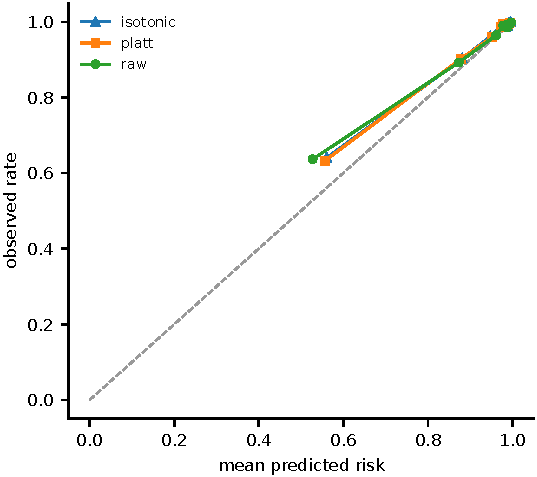
\includegraphics[width=0.72\linewidth]{figS7_calibration.pdf}
\caption{Calibration at the reference cell on the case study's log, by decile
of predicted risk. The two proper scoring rules on the metric axis --- Brier
skill and the log-loss skill --- read this picture; the two rank-based ones
cannot see it at all (Remark~\ref{prop:rank}). A pipeline whose
discrimination is adequate and whose calibration is not therefore moves the
increment on some instruments and not others, which is one concrete mechanism
behind the metric axis's contribution to Table~\ref{tab:sobol}.}
\label{fig:calibration}
\end{figure}

The frequency-encoded pipeline is the one that is visibly miscalibrated, with
a slope well below one, and it is also the one whose increment differs most
from the others on the two proper scoring rules. That is the interaction
between the pipeline axis and the metric axis, drawn.

Rolling-origin results are in \texttt{results/s01\_surface.csv} under
\texttt{split = rolling$k$} and enter the decomposition as the split axis;
Section~\ref{app:rolling} prints them per fold. The single holdout is not
the best estimate of the increment, and reporting it alone would be a
limitation.

\subsection{The case study's leakage and quality experiments}
\label{app:casedetail}

%%  ROUND TWENTY-SEVEN.  Section 7.3 was reduced to a stub and its prose
%%  moved here -- where round twenty-five had ALREADY put the full
%%  treatment of both experiments.  The move therefore duplicated, within
%%  one page, every number of the tipping point and the quality axis.  The
%%  moved copy is deleted and the round-25 block below stands; the body's
%%  stub summarises and points here, which is the arrangement round
%%  twenty-five chose and this pass should not have disturbed.

%%  ROUND TWENTY-FIVE.  Moved here from Section 7 unchanged.  The article
%%  keeps both findings and the pointer; the referees asked three times
%%  for a shorter article and this is detail, not evidence a reader needs
%%  in front of them.

\paragraph{The leakage tipping point}

The knowledge reference is load-bearing: it is the field that takes the
register's increment to indistinguishable from zero, so the evidence that it
was available at $\tau_2$ is stated exactly, and it is weaker than proof. The
interaction detail file establishes that the field is written by the
service-desk process and not by the incident process --- \nOrphans\
interactions in it never became incidents, and \kmOrphanPopulated\ of them
carry a knowledge reference --- but not \emph{when}, for a given incident, the
value was written. Table~\ref{tab:availability} lists each piece of evidence
beside what it does and does not establish. Availability at $\tau_2$ is
probable and unproven, and the disposition of an unprovable admissibility
assumption is a sensitivity analysis rather than a headline.



\begin{figure}[t]
\centering
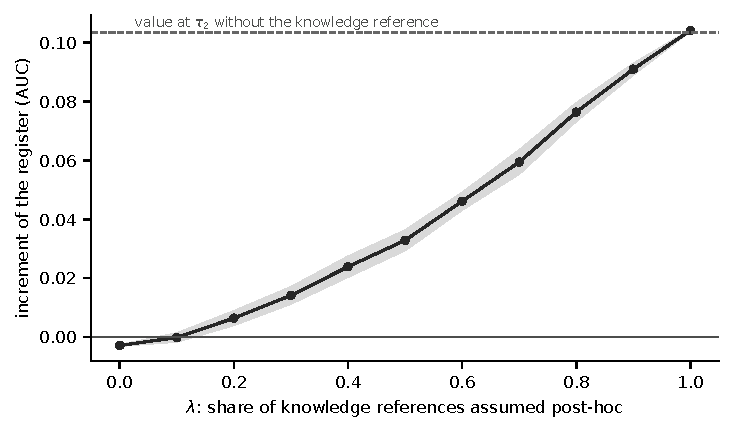
\includegraphics[width=0.82\linewidth]{figS5_tipping.pdf}
\caption{The register's increment at $\tau_2$ on the estate's cohort and
reassignment target, as a function of $\lambda$, the share of
knowledge-article references assumed to have been written after the incident
existed. A reader who has a belief about $\lambda$ can read their own answer
off the curve.}
\label{fig:tipping}
\end{figure}

Because availability is probable rather than proven, the increment is reported
in Figure~\ref{fig:tipping} as a function of $\lambda$, the share of knowledge
references assumed to have been written after the incident existed and
therefore inadmissible. Masking a
random $\lambda$ share of the field and re-estimating traces a curve from the
permissive end ($\lambda = 0$, the field fully admissible) to the conservative
end ($\lambda = 1$, equivalent to $\tau_2$ without the field at all). The
masking is stochastic, so each point is a mean over \nTippingSeeds\ seeds with
the spread across them printed beside it, and the curve is a sensitivity
display rather than an estimate the paper quotes a number from.

At $\lambda = 0$ the register is worth \VTtwoKnow\ [\VTtwoKnowLo,
\VTtwoKnowHi], which is not resolvably different from zero, and it reaches
half of its knowledge-free value at $\lambda = \lambdaHalf$: a reader who
believes that more than \lambdaHalfPct\ of knowledge references are written
\emph{after} the incident exists should read this estate's register as worth
at least half of \VTtwoGroup\ AUC, and one who believes almost none are should
read it as worth almost nothing. We have no way to measure $\lambda$ and do
not claim one; the curve makes the assumption explicit and continuous rather
than binary and made on the reader's behalf.


\paragraph{Register quality}


Masking a complete field is a sensitivity experiment, not a model of a real
register, so Table~\ref{tab:quality2} reports the \nQualityKinds\ mechanisms
of Section~\ref{sec:surface} plus a discovery lag, and sweeps the accuracy and
reconciliation mechanisms rather than reporting one level of each. Everything
here is on the estate's cohort and reassignment target;
Table~\ref{tab:quality3} carries the severity curves, over \nCaseSweepLevels\
severities and \nQualitySeeds\ seeds per stochastic mechanism, and
Table~\ref{tab:quality2corpus} the same mechanisms on the registered cohort.
Four things follow, and two of them are nulls we did not expect.

\textbf{Coverage is the expensive failure, and losing the long tail is not the
worst way to lose it.} At half population the register is worth \qRareHalf\ if
its long tail is absent and \qCommonHalf\ if its core is, against \qClean\
complete. Losing the core costs more than losing the tail, which is the
opposite of the usual intuition that the rare identities carry the
information: on this estate the frequent items are the ones the model has
enough cases to learn from. Loss at random is worse than either
(\qRandomHalf), because it fragments every identity rather than removing some
cleanly.

\textbf{Accuracy costs about what coverage costs.} Corrupting three tenths of
the identities --- the register is complete, and wrong --- leaves it worth
\qCorruptThirty, a loss of \qCorruptThirtyDelta, about what losing a third of
its population costs. A maturity assessment that counts populated rows and
does not sample them for correctness is measuring one of the two and reporting
it as the whole.

\textbf{Reconciliation failure is nearly free.} Splitting \emph{every}
identity into two records moves the increment by \qDuplicateAllDelta: with
thousands of cases per identity, halving the evidence behind each still leaves
enough.

\textbf{Staleness is exactly zero, and the reason is the encoder.} Removing
identities the register had not seen by the split point moves the increment by
\qStaleDelta. That is not a bug in the mechanism: a one-hot encoder fitted on
the training half already ignores levels it has never seen, so a test row
carrying an undiscovered identity contributes an all-zero encoding either way.
Under an encoder that keeps missingness as an explicit indicator the effect is
non-zero; Section~\ref{app:tables} measures that on the registered cohort.
A \emph{discovery lag} --- identities first used in the last half of the
training window absent everywhere, leaving \qLagHalfPopulated\ of rows
populated --- moves it by \qLagHalfDelta. Whether a data-quality defect is
visible is therefore an interaction between the quality axis and the encoding
axis, and an analyst who varies one without the other will conclude that the
defect does not matter.

\textbf{And which rows go missing matters as much as how many.} The three
\emph{dependent} mechanisms of Section~\ref{sec:surface} carry severity
integrals \integralTime, \integralContent\ and \integralPropensity, against
\integralMaskRare\ for the independent long-tail mechanism, which the
dependent ones bracket rather than track: the identity of the missing rows
changes what the loss costs by up to half again, so a quality axis built only
from independent coin flips is measuring one corner of the question. The
summary is an integral against a uniform measure on severity, and coarsening
the sweep from \nCaseSweepLevels\ severities to five moves it by at most
\gridShiftMaxCase\ AUC. Every mechanism is verified by execution to be a
function of the training half alone --- \nQualityLeakChecked\ checks run and
\nQualityLeakPassed\ pass.

\subsection{Calibration before the decision curve}
\label{app:dcadetail}

\textbf{Why that window, and why the exclusion is not repaired by
recalibrating again.} A Cox calibration slope of $\gamma$ means a threshold
$\theta$ selects the cases a well-calibrated model would select at a different
threshold, and the discrepancy grows without bound as $\gamma$ leaves one; the
window is the conventional band in which risks are neither compressed nor
stretched beyond a factor the literature treats as readable, and it is a
declared convention rather than a derived bound. Widening it to admit everything would not make the excluded thresholds
readable as cost ratios; it would only stop saying so. \textbf{Recalibration
is already an axis, which is why it cannot also be the remedy}: isotonic
recalibration is a level of the pipeline axis, so an arm that fails the slope
check has, on the pairs that carry it, a recalibrated sibling in the same
surface. Applying isotonic recalibration to the failing arm before excluding
it would silently replace one specification by another and report the result
under the first one's name --- the exact substitution this paper's argument is
against. The arm is excluded and its sibling is reported as itself.
The rule, what it removes and what the curves look like without it are
below.

%%  ROUND TWENTY-FIVE.  Moved here from Section 8 unchanged.

\paragraph{Calibration comes first, or the threshold means nothing}


The identity above reads $\theta$ as a probability threshold, and everything
that follows from it requires the score to be a probability. A threshold of
\thetaBase\ applied to a score whose calibration slope is \slopeWorstRaw\ is
not a statement about a cost ratio of \ratioBase\ false nominations per true
one; it is a statement about a number that happens to lie at \thetaBase\ on an
arbitrary scale. Every model contributing to a decision-curve conclusion in
this paper is therefore refitted under a \textbf{training-only} calibration:
isotonic and Platt scaling, each cross-validated \emph{inside} the training
half, so no test outcome touches the calibrator, and the calibration is
rebuilt inside every resampling iteration. Table~\ref{tab:calib2} gives the
diagnostics for the raw and the calibrated scores on every pair.

The correction bites. Across the corpus the median calibration slope is
\slopeRawMedian\ on raw scores and \slopeIsoMedian\ after isotonic
calibration; the median expected calibration error falls from \eceRawMedian\
to \eceIsoMedian; and the number of arms whose slope lies outside $[0.5, 2]$
falls from \nSlopeOutRaw\ to \nSlopeOutIso. It also changes conclusions: the
sign of the net-benefit increment differs between the raw and the calibrated
curve at a mean \dcaSignChangePct\ of thresholds.

\textbf{What may and may not be read as a decision curve.} Curves computed on
calibrated probabilities carry the probability-threshold interpretation and
are what Section~\ref{sec:dcabands} and the case study read. Curves on raw
scores are reported as \emph{score-threshold sensitivity analyses} and are
labelled so in every table; they say how a conclusion moves as a selection
rule tightens, and they do not say what cost ratio that rule encodes.

\subsection{Simultaneous bands on the decision curve}
\label{app:dcabandsfull}

%%  ROUND TWENTY-FIVE.  Moved here from the article for length, unchanged.

\begin{figure}[t]
\centering
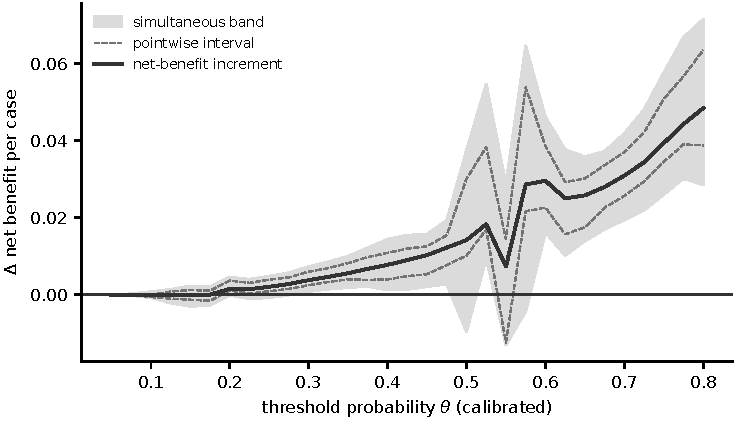
\includegraphics[width=0.92\linewidth]{figS4_dca.pdf}
\caption{The register's net-benefit increment across the operating range at
the reference cell, with the pointwise interval and the simultaneous max-$t$
band. The simultaneous band is what a claim about a \emph{range} of thresholds
has to be read against. \textbf{The band drawn here is the multiplier's
nominal one}: the band the article's counts are read against is the
admissible empirical quantile's (Section~\ref{sec:dcabands}), wider at every
point, and the earlier construction that widened the nominal band by a
measured \dcaWidenFactor\ is kept in the text below as a comparison, so this
figure shows the shape of the curve and the ordering of the two intervals,
and not the band any claim is read against. The curve dips near $\theta = \dcaDipTheta$ as drawn,
where the nominal band's lower edge reaches \dcaDipValue\ --- under the widened
band the dip is at $\theta = \dcaDipThetaWidened$ and reaches
\dcaDipValueWidened. Either way the dip is not a harm the evidence resolves:
\nHarmfulPointwise\ of the \nDcGrid\ operating points resolve as harmful
pointwise, \nHarmfulSimultaneous\ under the nominal band and
\nHarmfulSimultaneousWidened\ under the widened one.}
\label{fig:dca}
\end{figure}

Figure~\ref{fig:dca} draws the register's net-benefit increment across the
grid at the reference cell on \emph{calibrated} probabilities, with the
pointwise interval and the simultaneous max-$t$ band. The band's family is
declared separately from the scalar family and spans every admissible
net-benefit cell of the pair, \nDcaFamily\ members. The band the article
reports (Section~\ref{sec:dcabands}) uses the admissible empirical quantile
\dcaQEmp\ (\dcaQEmpAll\ with the degenerate cells kept); the ladder in this section also carries an earlier construction,
the multiplier's nominal value \dcaQ\ widened by a measured factor
\dcaWidenFactor\ to \dcaQWidened, as the comparison, and the difference
from a pointwise reading is not cosmetic under either. Under the widened
construction the median width is
\dcBandWidthWidened\ against the pointwise interval's
\dcPointWidth\ (\dcBandWidth\ before the widening), and across the
\nDcGrid\ operating points of this estate's
decision curve the pointwise interval declares the increment resolvably
positive at \nBeneficialPointwise\ of them while the simultaneous band
declares it at \nBeneficialSimultaneousWidened\
(\nBeneficialSimultaneous\ under the nominal band). Both are built from the same draws,
so the only thing that differs is the family: those points are the price of a
statement about a \emph{range} of thresholds rather than about each threshold
separately, and a paper that reads a decision curve across its range and
prices it pointwise has claimed the first while paying for the second.

The curve dips near $\theta = \dcaDipThetaWidened$, where the widened band's
lower edge reaches \dcaDipValueWidened, so the count of points that resolve as
\emph{harmful} is reported rather than left to the eye:
\nHarmfulPointwise\ of the \nDcGrid\ points pointwise and
\nHarmfulSimultaneousWidened\ under the simultaneous band. The second can only be
smaller than or equal to the first --- the wider family gives the wider
interval at every point, which the verifier checks --- so a dip a
reader can see is not a harm the evidence resolves. Over the
\nDcaFamily\ cells of the band's own family --- \emph{not} the
\nDcaRows\ decision-curve rows the corpus carries as point estimates, which
are a different and much larger set --- the same counts are
\dcaHarmfulPointwise\ and \dcaHarmfulSimultaneousWidened; Table~\ref{tab:dca} prints
this pair's own curve, operating point by operating point, and its caption
names the cell it is computed at.

\textbf{This family is the one most exposed to how the critical value is
estimated, and it is the one where the estimator matters most.} On every
one of the \nFamiliesDca\ decision-curve families the multiplier value lies
below the whole order-statistic interval of the empirical quantile
(Section~\ref{sec:simbands}), by a median factor of \qRatioDcaMedian, and
across the corpus's decision-curve cells the multiplier band would resolve
\nResolvedDcaMult\ against the empirical band's \nResolvedDcaEmp. Part of
that ratio is arithmetic rather than tail: cells that are exactly zero in at
least nine draws of ten inflate the empirical quantile of any family that
keeps them, which is why the article's rule excludes them before the
quantile is taken and prints the excluded count (\nDcaCellsExcludedDegenerate\
of \nDcaFamily\ on this family). The measured widening of
\dcaWidenFactor\ that an earlier construction applied to the multiplier
value is kept in the ladder above as the comparison: it lands at
\dcaQWidened\ against the admissible empirical quantile's \dcaQEmp, and the
counts under it are printed so the reader can see that the two agree on the
shape of the conclusion and differ on its size. The $(n,K)$ calibration of
Section~\ref{sec:regions} is estimated for the scalar instruments and is not
applied here either.

\subsection{The ITSM family, statistic by statistic}
\label{app:itsmfamily}

%%  ROUND TWENTY-FIVE.  Moved from the article for length, unchanged.

Eight of the \nPairs\ pairs are IT service management, where the register is a
maintained configuration or customer register and a data-quality mechanism has
an operational referent. The other eleven include a loan amount treated as a
high-cardinality categorical, a case-type reference nobody curates and an
article of law, which Section~\ref{app:construct} names as threats to
construct validity. Table~\ref{tab:family} reports every headline statistic on
all nineteen pairs, on the eight, and on the eleven that remain, each with a
cluster-bootstrap interval taking the \emph{log} as the resampling unit ---
two targets on the same log share a cohort and are not two independent
observations.

The higher-order share is \itsmHigherOrderPct\ on the ITSM family against
\interactionTotalPct\ on the whole corpus, the largest first-order index
\itsmLargestFirstOrderPct\ against \largestFirstOrderPct, and the all-cells
sign-disagreement rate \misreportItsmPct\ against \misreportEqualPct. One
difference runs against the paper. \textbf{The headline is lower on the
population this paper is about}: of the resolved cells,
\misreportPooledItsmPct\ disagree in sign on the ITSM family against
\misreportPooledOtherPct\ on the other eleven and
\misreportPooledResolvedPct\ pooled. The corpus-wide figure is therefore
driven by the pairs Section~\ref{app:construct} names as carrying
construct-validity threats, and a reader who takes this paper to be about
maintained registers should read the ITSM column and should read it as the
weaker case for the apparatus, not the stronger one.

\subsection{The desk's decision, in net benefit per thousand}
\label{app:deskfull}

%%  ROUND TWENTY-FIVE.  Moved from the article for length, unchanged.

Because net benefit is a single cardinal utility, the decision-rule comparison
of Section~\ref{sec:rules} can be run on it without the unit problem that
forces that section to work instrument by instrument. Three things have to be
settled first, and each is settled by a declared rule rather than a default.

\textbf{Which models may enter.} A threshold is a cost ratio only if the score
is a probability, so a model whose recalibrated slope lies outside
$[\slopeLo, \slopeHi]$ is excluded from the decision-analytic reading by a
registered rule applied at the level of the (pair, pipeline, baseline) triple
and requiring both arms to pass. A \emph{model} here is one such triple,
not one fitted classifier. The rule removes \nModelsDcaExcluded\ of
\nModelsDca\ of them and leaves \nPairsDcaExcluded\ of \nPairs\ pairs
with none. \textbf{That count is itself the strongest operational finding in this
section}: on a third of the models a published evaluation would fit here, no
threshold can be read as a cost ratio at all.

\textbf{Which thresholds.} A uniform measure over an operating range from
$0.05$ to $0.80$ is not a desk's belief. For a decision about pre-empting a
reassignment the false positive costs a specialist's few minutes and the false
negative costs a re-triage, a second queue wait and the service-level exposure
that goes with it; ratios between three and ten to one put the indifference
threshold between \deskQlo\ and \deskQhi, with a median of \deskQmid. A Beta
distribution with that support is declared as the \emph{desk distribution},
and single exchange rates are reported beside it.

\textbf{Which unit.} Net benefit per case is a rate near zero, and three
decimal places of it look like a tie, so Table~\ref{tab:desk} reports it per
thousand cases.

\textbf{And where the rules separate, what separates is the conservative
rule.} Under the desk distribution the
one-number rule, the majority rule and the weighted mean all carry a median
excess regret of \excessOneNumberDesk\ per thousand cases; only the
conservative rule loses, at \excessUniformDesk\ --- and the medians hide a
tail that is entirely that rule's, whose cross-pair \emph{mean} excess is
\meanExcessUniformDesk\ against the one-number rule's
\meanExcessOneNumberDesk. The four rules do not all lose the same amount on
\nSeparatingDesk\ of the \nPairsDesk\ pairs the calibration rule admits, and
are identical on the other \nAllRulesTieDesk. Where they do separate the
one-number rule is strictly the worst on \nOneNumberWorstDesk\ and tied for
worst on \nOneNumberTiedWorstDesk, at a maximum of
\maxExcessOneNumberDesk\ per thousand --- a real ordering and a small
quantity. \textbf{The case against a one-number report does not rest on this
design.} It rests on the decomposition of Section~\ref{sec:sobol} and on the
sign disagreement of Section~\ref{sec:results-regret}, which is unit-free.

\textbf{What does separate, in this unit, is the forecast origin.} The register
is worth \promisedPerThousand\ true positives per thousand cases against the
intake block. Against intake plus group plus the knowledge reference --- the
same estate, the same register, a later moment in the same process --- it is
worth \deliveredPerThousand. A desk that read the first number and deployed
where the second applies is short \shortfallPerThousand\ per thousand cases.
That is the operational content of Section~\ref{sec:twodecision}, and it is
larger than the most the choice of collapse rule costs a one-number report,
which is \maxExcessOneNumberDesk\ per thousand at its worst pair. It is
\emph{not} larger than every difference between the four rules: the
conservative rule's own mean excess is \meanExcessUniformDesk\ per thousand,
which exceeds it, and that rule reaches far more than this on a single pair.
The comparison that holds is against the rule this section is about, and it is
stated at that width rather than at the one that reads better.
It is also conditional on the knowledge reference being admissible at
$\tau_2$, which Section~\ref{sec:cmdb} shows is probable and unproven: the
second figure is the $\lambda = 0$ end of Figure~\ref{fig:tipping}, and a reader
who believes a share $\lambda$ of those references are written after the incident
exists should read their own figure off that curve.

\paragraph{What the operational statement does not say} Net benefit converts a
discrimination increment into units the desk recognises. It does not convert
it into money, and three gaps remain, each needing data this study does not
have: nominating a case for review is not the same as preventing a
reassignment, and whether acting on a nomination changes the outcome is an
interventional question on observational evidence; the exchange rate is
declared rather than measured, which is why the whole curve is reported; and
the cost of the register itself --- discovery tooling, reconciliation effort,
the staff who keep it current --- is nowhere in this evidence.

\subsection{The measure, the target axis, and which axis leads}
\label{app:measures}

%%  ROUND TWENTY-SEVEN.  Moved from Section 6.2 for length, unchanged.

\textbf{The pooled decomposition, for comparison.} Across the corpus the
median pooled first-order index is \sSplitPct\ for the split, \sRungPct\ for
the baseline rung, \sQualityPct\ for the register-quality condition and
\sLearnerPct\ for the pipeline; at the median pair the largest first-order
index \emph{within an instrument} --- a median over pairs of a median over
instruments, and not the largest of those four medians --- is
\largestFirstOrderPct, the total higher-order share is \interactionTotalPct\
(\interactionTotalCI\ over pairs, \interactionMinPct\ to
\interactionMaxPct), and the largest per-axis \emph{involvement}
$\max_i (S_{T_i} - S_i)$, a different quantity, is \largestInvolvementPct.
The involvement is reported because it is what the specification-curve
literature computes, and because the difference between it and the
higher-order share is what Section~\ref{sec:axes2} turns on --- not because it
answers the question as asked.


%%  ROUND TWENTY-FIVE.  Moved from Section 6.2 for length, unchanged.

\textbf{The measure is not neutral, and one conclusion does not survive it.}
Under the reference-weighted measure the median higher-order share is
\interactionTotalReferencePct\ and under the concentrated measure
\interactionTotalConcentratedPct\ (Table~\ref{tab:measures}). That second
number is smaller than the largest first-order index under the same measure,
\concentratedFirstOrderPct, and on \nConcentratedExceeds\ of \nPairs\ pairs
some single axis carries more variance than everything higher-order combined
--- against \nEqualExceeds\ pairs under the equal-level measure. The statement
\emph{the interactions carry more than any main effect} is therefore true
under the two measures that let a reader roam and false under the one that
keeps them near the reference cell. Both invariance tests pass, to
\invarianceDuplicateShift\ and \invarianceGridShift.

\textbf{The target is an axis too, and it is a small one within a pair.} Every
index above is computed \emph{within} a log--target pair. On the
\nLogsBothTargets\ logs carrying both registered targets the target axis can
be added, on the headroom scale, and it carries a median \sobolTargetPct. The
two targets are different questions, agreeing on a median \targetAgreement\ of
cases, so the reading is not that the target hardly matters --- on the case
study it decides the sign (Section~\ref{sec:cohort}) --- but that once it is
fixed, the remaining choices move the answer by more than switching it does.

\textbf{Which axis leads is a property of the pair.} The largest single
first-order index anywhere on the corpus is \topIndexPct, carried by
\topIndexAxis\ on \topIndexPair; \nAxesLeading\ different axes lead somewhere,
and the most frequent leader is \modalLeadingAxis, on
\modalLeadingSharePct\ of pair--instrument combinations. An analyst can guess
the leader and be right about half the time.

\subsection{What the pooled resolved rate is a ratio of}
\label{app:pooled}

%%  ROUND TWENTY-FIVE.  Moved from Section 6.5 for length, unchanged.

\textbf{It is a pooled ratio, it depends on which band resolves the cells, and
both facts belong beside it.} The denominator is a sum over pairs whose
resolved-cell counts run from zero to \nResolvedMax, not an average of
per-pair rates, and it depends on which band decides what ``resolved'' means.
The figure quoted here, \misreportPooledResolvedPct, is the reported
band's --- the empirical critical value, with no $(n,K)$ widening applied
(Section~\ref{sec:simband}). The estimator choice moves it: under the
multiplier approximation the denominator is larger, \nResolvedWholeMult\
cells against the reported band's \nResolvedWholeEmp. \textbf{And the
disagreements are concentrated}: of the
\nDisagreeResolved\ cells, \nDisagreeTopThree\ come from three logs, and only
\nLogsDisagree\ of the \nLogs\ logs contribute any at all. The designed surface runs every pair at the same draw count, so unlike
earlier reports of this statistic the concentration cannot be a budget effect. On \nPairsNoResolvedDisagreement\ pairs no resolved
cell contradicts the reference, on \nPairsSomeResolvedDisagreement\ some do,
and on \nPairsNoResolvedCell\ nothing resolves.

\subsection{What this says to a configuration management programme}
\label{app:programme}
\label{sec:csdm}

%%  ROUND TWENTY-FIVE.  Moved from the article for length, unchanged.

The register in this log is layered, and the layers are the ones a common
service data model uses: an item belongs to a class, a class to a subtype, and
a subtype rolls up to a service component. Section~\ref{app:layers}
estimates the increment at each layer against the intake block, on the
registered targets. The coarse layers are \emph{not} free --- on the handover
target the item's type alone is worth \layerTypeHandover\ and its subtype
\layerSubtypeHandover, against \layerItemHandover\ for the item itself, and on
duration \layerTypeDuration\ against \layerItemDuration\ --- so knowing that a
case concerns \emph{a laptop} is worth between a third and two thirds of
knowing which one. What the item adds \emph{on top of} the subtype is the
quantity a populated hierarchy does not buy, and it is
\layerItemMarginalHandover\ on handover and \layerItemMarginalDuration\ on
duration. A programme that populates the class hierarchy and stops has bought
a real part of the value and left the larger marginal part on the table; it
has not bought nothing. These figures are on the registered targets rather
than the reassignment target of the case study in Section~\ref{sec:cmdb},
and Section~\ref{app:layers} says so.

The three dependent quality mechanisms map onto how a configuration management
database actually decays, which is why they are in the design space rather
than independent coin flips. \emph{Discovery lag} is the interval between a
service going live and the discovery tooling finding its items, which is why a
new service's cases carry an empty affected item for weeks. \emph{Unreconciled
duplicates} arise when two discovery sources write the same physical item
under two identifiers. \emph{Propensity-dependent missingness} arises when the
affected item is populated by the desk rather than by discovery: the unusual
case, which is the one worth predicting, is the one the desk is least likely
to classify correctly under time pressure. The measured costs above say which
of the three is worth spending on: on this estate, coverage and accuracy at
the item level, and not reconciliation.

Two disclaimers. This is forecast performance on one estate for one
decision, not procurement advice, and a register that pays nothing here may be
bought for change control, audit or impact analysis, none of which this
measures; and the ranking of the mechanisms is a property of this cohort's
cardinality and volume.

\subsection{The three forecast origins, moment by moment}
\label{app:taudetail}

%%  ROUND TWENTY-FIVE.  Moved from Section 7.2 for length, unchanged.

An incident in this estate does not begin as an incident. A caller reaches the
service desk, an \emph{interaction} is opened, the desk works it, and if it
cannot be closed there an incident is created and routed. Three moments at
which a prediction could be made are estimated, and what changes between them
is not only which fields are admissible (Table~\ref{tab:tau}).

\begin{description}
\item[$\tau_0$, first touch, every call.] The desk has just picked up the
call and does not yet know whether it will escalate. The population is every
interaction --- \nTauZero\ of them --- the register is the interaction's own
affected item, with \cardTauZero\ values, and the admissible baseline is the
interaction's intake block. Against it the register is worth \VtauZero\
[\VtauZeroLo, \VtauZeroHi].
\item[$\tau_1$, first touch, the calls that escalate.] The same moment and
the same fields, restricted to the \nTauOne\ calls that did become incidents.
The register is worth \VtauOne\ [\VtauOneLo, \VtauOneHi].
\item[$\tau_2$, incident creation.] The desk has worked the interaction and
escalated it. The population is the \nTauTwo\ incidents; the group that logged
the incident is known, and so --- probably --- is the knowledge-article
reference the desk consulted. Against the intake block the register is worth
\VtauTwo; against intake plus group, \VTtwoGroup\ [\VTtwoGroupLo,
\VTtwoGroupHi]; against intake plus group plus the knowledge reference,
\VTtwoKnow\ [\VTtwoKnowLo, \VTtwoKnowHi] --- the one rung of the five that
does not resolve.
\end{description}

The pairwise differences separate the mechanisms that a baseline ladder alone
conflates, and separating them properly requires one more row than the three
moments give. $\tau_1$ and $\tau_2$ are \emph{not} the same cases:
\nTauTwoUnmatched\ incidents have no interaction record, so $\tau_2$ carries
\nTauTwo\ cases against $\tau_1$'s \nTauOne. Table~\ref{tab:tau} therefore
also reports $\tau_2$ restricted to $\tau_1$'s own population --- the same
\nTauTwoMatched\ cases at the same prevalence \prevTauOne\ --- which is the
row that makes the information step an information step.

Restricting the population from every call to the calls that escalate, holding
the information fixed, moves the increment by \deltaCohortAtTau\ AUC. Moving
from first touch to incident creation \emph{on the matched cases}, changing
what is known and nothing else, moves it a further \deltaSnapshotAtTau. The
remaining \deltaPopulationResidual\ is what the \nTauTwoUnmatched\ incidents
with no interaction record are worth, and it is a population difference rather
than an information one: the unadjusted $\tau_1$-to-$\tau_2$ step,
\deltaSnapshotUnmatched, is the sum of the two and attributing all of it to
information would overstate the information channel by three quarters.
Admitting the group and then the knowledge reference takes the increment the
rest of the way to zero. A forecast origin is therefore an argument of the
estimand in its own right: it fixes the population, the feature snapshot and
the admissible set, and only the third of those is a baseline.

Neither $\tau_0$ nor $\tau_2$ is ``the'' answer: which one a reader wants
depends on where in their own process they intend to predict. A desk screening
at $\tau_0$ looks at \nTauZero\ calls a year at a prevalence of \prevTauZero;
a desk screening at $\tau_2$ looks at \nTauTwo\ incidents at \prevTauTwo, and
Section~\ref{sec:nbregret} prices the difference.

\subsection{Magnitude weighting, and the rate under each measure}
\label{app:magnitude}

%%  ROUND TWENTY-FIVE.  Moved from the article for length, unchanged.

\textbf{Weighting by magnitude does not rescue the conventional report, and
the rate depends on the measure.} Weighting each cell by $|V|$ as well as by
the measure gives a median \misreportMagnitudePct, \emph{higher} than the
unweighted rate: the cells that disagree are not the negligible ones. The
median is \misreportEqualPct\ under the equal-level measure,
\misreportReferencePct\ under the reference-weighted and
\misreportConcentratedPct\ under the concentrated, falling as the measure
concentrates on the reference specification, which is what it should do. A
sign comparison is unit-free, which is why this one quantity may be pooled
across instruments where an expected loss may not.

Table~\ref{tab:regret} attributes the disagreement to axes. Holding everything
else fixed and changing one axis, the sign of the increment flips for a median
\flipSplitPct\ of same-everything-else pairs of cells under the split,
\flipLearnerPct\ under the pipeline, \flipRungPct\ under the baseline rung,
\flipQualityPct\ under the register-quality condition and \flipMetricPct\
under the metric. The two axes an evaluation paper is most likely to hold
fixed without comment --- which split, which pipeline --- are the two that
flip the sign most often.

\subsection{The eight pairs where the construct is what this paper is about}
\label{sec:family}

Every corpus statistic is reported on the \nItsmPairs\ ITSM-like pairs as
well as on all \nPairs\ (Table~\ref{tab:family}), because the register there
is a maintained one and the construct is what the paper is about.
\textbf{The headline is lower on the population this paper is about}: the
sign-disagreement rate is \misreportItsmPct\ against \misreportEqualPct\ over
the corpus, and on resolved cells \misreportPooledItsmPct\ against
\misreportPooledOtherPct\ on the rest. The decomposition barely moves ---
higher-order \itsmHigherOrderPct\ against \interactionTotalPct, largest
first-order \itsmLargestFirstOrderPct\ against \largestFirstOrderPct.
Section~\ref{app:itsmfamily} carries every statistic on both populations.

\subsection{The one surface that is uniformly beneficial, and what it cost to
reach}
\label{app:uniformly}

\textbf{\nUniformlyBeneficial\ of the \nPairs\ pairs is uniformly
beneficial, and the interesting part is the denominator.} The label requires
every cell of the \emph{inference family} to have its lower band above zero
(Definition~\ref{def:regions}) --- a set that is a median
\inferenceShareAdmissibleMedianPct\ of a pair's admissible cells, and on the
pair that reaches the label it is smaller still, under a twentieth. A label
about \emph{every} cell is correspondingly easier to earn over fewer of them,
which is why Section~\ref{sec:regionsdef} names this as the label the
restriction most flatters.

\noindent It is not, however, an artefact of the critical value. A cell
whose point estimate is negative can never qualify at any critical value,
and the pair in question carries none inside its family; the label holds
under the multiplier, under the empirical quantile the article reports,
under its order-statistic upper end and under every widening the $(n, K)$
calibration could ask for (Section~\ref{app:foursettings}). So the state
is genuinely reached, and reached over \shareUniformFamilyPct\ of the
specifications the declaration admits.

\noindent \textbf{That combination is the point rather than an
embarrassment.} Section~\ref{sec:regionsdef} offers $\rho = 1$ as the only
state in which one positive number is a safe summary of a surface, and asks
how often it obtains. It obtains once here --- on the pair with the richest
declared grid --- and the claim it licenses ranges over \shareUniformFamilyPct\
of that pair's admissible specifications. A reader who wants a single number for this
register may have one, provided they are content that it is a statement about
the design the band was computed on and not about the design they might have
declared.

\noindent The statement that needs none of the apparatus is the weaker one
that survives everywhere: on every pair at least one admissible specification
has a negative increment, which is visible from the all-cells column of
Table~\ref{tab:misreport}. What the apparatus earns is $\rho$ and the
resolved counts.

%%  ROUND TWENTY-FIVE.  Moved from Section 6.4 for length; Table~\ref{tab:master}
%%  carries the same rho per pair.

\begin{figure}[t]
\centering
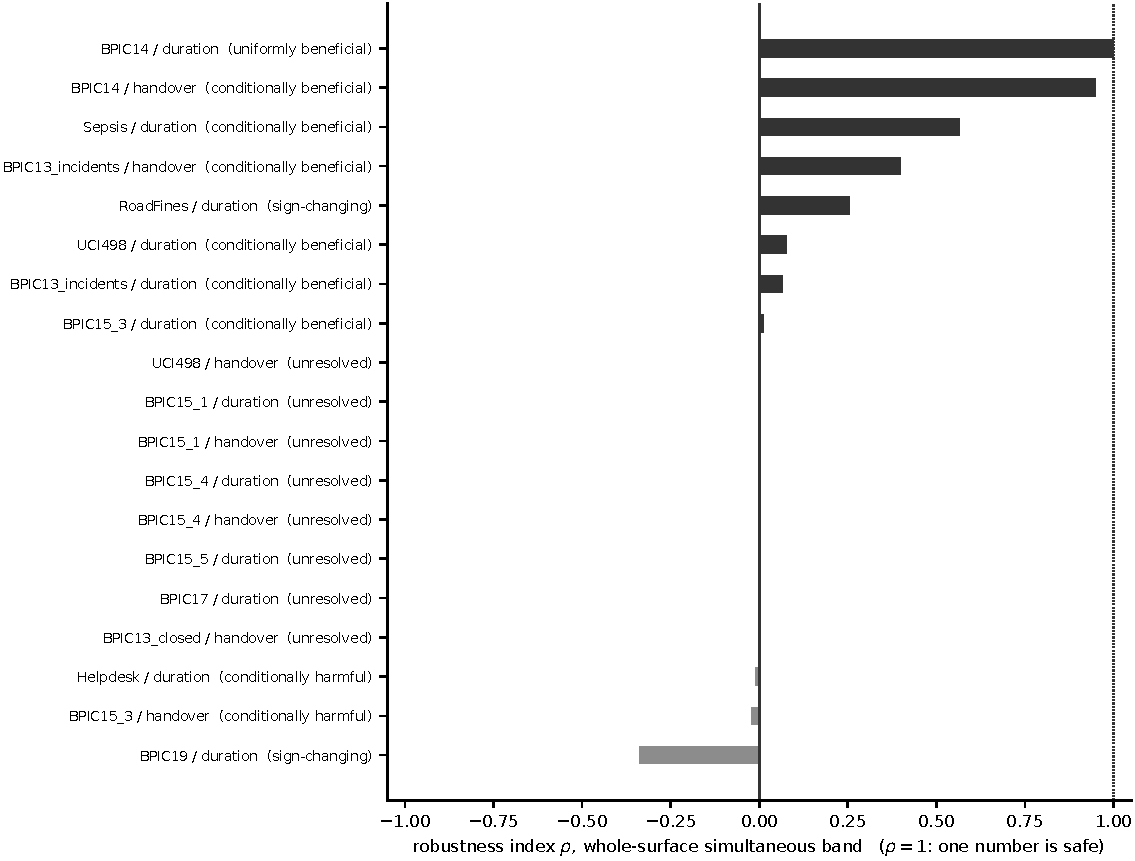
\includegraphics[width=0.92\linewidth]{figS3_regions.pdf}
\caption{The robustness index $\rho$ per log--target pair, with the region
label, at the critical value Section~\ref{sec:regions} reports. The label
drawn here is the one the band yields \emph{before} the minimum resolved
share of Definition~\ref{def:regions}, which changes it on
\nMarkedBelowMinShare\ of these pairs (Table~\ref{tab:triple}). $\rho = 1$,
the dotted line, is the only state in which a single positive number is a safe
summary.}
\label{fig:regions}
\end{figure}


\subsection{How much of the rung spread the half-of-intake rung carries}
\label{app:spread}

%%  ROUND TWENTY-SEVEN.  Moved from Section 6.2 for length, unchanged.

\textbf{How much of the range the half-of-intake rung
carries is itself a property of the pair}: dropping it cuts the spread by a
median \spreadFallMedianPct\ per pair, by \spreadFallWidestPct\ on the pair
holding the corpus's widest spread, and not at all on \nPairsSpreadUnmoved\
pairs, where the rung's own increment falls inside the range the remaining
rungs already span. The fall is not a correction of an error but
a change of denominator with a plain explanation: on
\nPairsTwoRealisticRungs\ of the \nPairs\ pairs only two rungs remain, so the
spread over them \emph{is} the absorption $D$ of the free field, which
Section~\ref{app:absorption} reports as an object in its own right with its
own interval. Only the case study's log carries a third
(Table~\ref{tab:roles}), and its two pairs are where the corpus's widest
realistic-rung spread sits, reaching \spreadRealisticMax.


\section{Tables the article summarises}
\label{app:tables}
The article prints the \nArticleTables\ tables a reader needs to follow its
argument.
This section carries the ones it summarises: the exclusion ledger, the
construct audit, the surface denominator, the planned contrasts, the region
labels, the ITSM family split, the sign-flip attribution, the cohort
decomposition, the axis-kind partition, the specification-curve comparison,
the desk utility, the tipping curve, the decision-curve corpus, the declared
measures, the four decision rules, the calibration diagnostics, the
availability evidence, the severity sweeps, the absorption ladders, and the
simulation in full. Every one is generated by
\texttt{scripts/make\_numbers.py} from the result files, and none is typed by
hand.

\subsection{The corpus}

Tables~\ref{tab:sobol} to~\ref{tab:confirm}: the within-instrument
sensitivity decomposition, the calibrated resolution regions, the
sign-disagreement rate counted three ways, the reconciliation of the two
published values, the exclusion ledger, the construct audit, the surface
denominator audit and the five planned contrasts.

\begin{table}[t]
\centering
\small
\resizebox{\ifdim\width>\linewidth\linewidth\else\width\fi}{!}{%%
\begin{tabular}{llrrrrrr}
\toprule
log & target & learner & quality & rung & split & higher-order total & largest involvement \\
\midrule
BPIC13\_closed & handover & 0.110 & 0.029 & 0.075 & 0.203 & 0.560 & 0.437 \\
BPIC13\_incidents & duration & 0.036 & 0.029 & 0.029 & 0.384 & 0.409 & 0.372 \\
BPIC13\_incidents & handover & 0.024 & 0.099 & 0.169 & 0.172 & 0.308 & 0.251 \\
BPIC14 & duration & 0.242 & 0.151 & 0.359 & 0.013 & 0.233 & 0.180 \\
BPIC14 & handover & 0.314 & 0.127 & 0.307 & 0.010 & 0.233 & 0.183 \\
BPIC15\_1 & duration & 0.041 & 0.039 & 0.055 & 0.263 & 0.614 & 0.548 \\
BPIC15\_1 & handover & 0.018 & 0.036 & 0.075 & 0.079 & 0.575 & 0.476 \\
BPIC15\_3 & duration & 0.003 & 0.081 & 0.025 & 0.287 & 0.607 & 0.490 \\
BPIC15\_3 & handover & 0.002 & 0.004 & 0.128 & 0.189 & 0.662 & 0.547 \\
BPIC15\_4 & duration & 0.060 & 0.025 & 0.011 & 0.111 & 0.732 & 0.655 \\
BPIC15\_4 & handover & 0.022 & 0.031 & 0.035 & 0.050 & 0.793 & 0.643 \\
BPIC15\_5 & duration & 0.078 & 0.042 & 0.057 & 0.036 & 0.749 & 0.664 \\
BPIC17 & duration & 0.000 & 0.062 & 0.001 & 0.346 & 0.590 & 0.494 \\
BPIC19 & duration & 0.014 & 0.011 & 0.003 & 0.491 & 0.474 & 0.418 \\
Helpdesk & duration & 0.262 & 0.086 & 0.008 & 0.222 & 0.339 & 0.314 \\
RoadFines & duration & 0.009 & 0.289 & 0.032 & 0.192 & 0.449 & 0.424 \\
Sepsis & duration & 0.021 & 0.145 & 0.008 & 0.134 & 0.608 & 0.574 \\
UCI498 & duration & 0.048 & 0.030 & 0.056 & 0.399 & 0.433 & 0.391 \\
UCI498 & handover & 0.079 & 0.071 & 0.287 & 0.136 & 0.390 & 0.285 \\
\bottomrule
\end{tabular}%
}
\caption{The corrected sensitivity decomposition, within instrument, under the equal-level measure. The four first-order indices, then the TOTAL higher-order share $1-\sum_i S_i$ of Equation~\eqref{eq:inttotal} of the article, then the largest per-axis interaction involvement $\max_i(S_{T_i}-S_i)$ --- which is the quantity an earlier version reported as the interaction share and which is not it, because those differences overlap across axes.}
\label{tab:sobol}
\end{table}


\begin{landscape}
\begin{table}[t]
\centering
\small
\resizebox{\ifdim\width>\linewidth\linewidth\else\width\fi}{!}{%%
\begin{tabular}{llrrrrrlrlrl}
\toprule
log & target & K / n & q (multiplier) & q (operative) & c & q calibrated & cells (nominal) & rho & cells (cal) & rho (cal) & region (cal) \\
\midrule
BPIC13\_closed & handover & 0.324 & 3.380 & 4.209 & 1.767 & 7.437 & 0 / 0 / 180 & 0.000 & 0 / 0 / 180 & 0.000 & unresolved \\
BPIC13\_incidents & duration & 0.133 & 3.372 & 4.138 & 1.456 & 6.027 & 12 / 0 / 168 & 0.067 & 2 / 0 / 178 & 0.011 & conditionally beneficial \\
BPIC13\_incidents & handover & 0.133 & 3.356 & 4.433 & 1.456 & 6.456 & 72 / 0 / 108 & 0.400 & 49 / 0 / 131 & 0.272 & conditionally beneficial \\
BPIC14 & duration & 0.093 & 3.214 & 3.709 & 1.294 & 4.798 & 180 / 0 / 0 & 1.000 & 180 / 0 / 0 & 1.000 & uniformly beneficial \\
BPIC14 & handover & 0.093 & 3.266 & 4.768 & 1.294 & 6.168 & 171 / 0 / 9 & 0.950 & 152 / 0 / 28 & 0.844 & conditionally beneficial \\
BPIC15\_1 & duration & 0.106 & 3.362 & 5.485 & 1.343 & 7.368 & 0 / 0 / 180 & 0.000 & 0 / 0 / 180 & 0.000 & unresolved \\
BPIC15\_1 & handover & 0.106 & 3.377 & 6.084 & 1.343 & 8.171 & 0 / 0 / 180 & 0.000 & 0 / 0 / 180 & 0.000 & unresolved \\
BPIC15\_3 & duration & 0.095 & 3.362 & 4.667 & 1.300 & 6.066 & 2 / 0 / 178 & 0.011 & 0 / 0 / 180 & 0.000 & unresolved \\
BPIC15\_3 & handover & 0.095 & 3.345 & 5.032 & 1.300 & 6.541 & 0 / 4 / 176 & $-$0.022 & 0 / 3 / 177 & $-$0.017 & conditionally harmful \\
BPIC15\_4 & duration & 0.072 & 3.409 & 5.847 & 1.243 & 7.270 & 0 / 0 / 180 & 0.000 & 0 / 0 / 180 & 0.000 & unresolved \\
BPIC15\_4 & handover & 0.072 & 3.430 & 6.068 & 1.243 & 7.545 & 0 / 0 / 180 & 0.000 & 0 / 0 / 180 & 0.000 & unresolved \\
BPIC15\_5 & duration & 0.132 & 3.407 & 5.777 & 1.455 & 8.405 & 0 / 0 / 180 & 0.000 & 0 / 0 / 180 & 0.000 & unresolved \\
BPIC17 & duration & 0.032 & 3.276 & 5.172 & 1.177 & 6.086 & 0 / 0 / 180 & 0.000 & 0 / 0 / 180 & 0.000 & unresolved \\
BPIC19 & duration & 0.011 & 3.380 & 5.808 & 1.177 & 6.834 & 10 / 71 / 99 & $-$0.339 & 8 / 60 / 112 & $-$0.289 & sign-changing \\
Helpdesk & duration & 0.123 & 3.325 & 3.931 & 1.431 & 5.625 & 0 / 2 / 178 & $-$0.011 & 0 / 0 / 180 & 0.000 & unresolved \\
RoadFines & duration & 0.001 & 3.298 & 5.063 & 1.177 & 5.958 & 52 / 6 / 122 & 0.256 & 46 / 6 / 128 & 0.222 & sign-changing \\
Sepsis & duration & 0.200 & 3.319 & 3.911 & 1.562 & 6.112 & 102 / 0 / 78 & 0.567 & 11 / 0 / 169 & 0.061 & conditionally beneficial \\
UCI498 & duration & 0.301 & 3.296 & 4.010 & 1.756 & 7.040 & 14 / 0 / 166 & 0.078 & 2 / 0 / 178 & 0.011 & conditionally beneficial \\
UCI498 & handover & 0.301 & 3.339 & 5.506 & 1.756 & 9.666 & 0 / 0 / 180 & 0.000 & 0 / 0 / 180 & 0.000 & unresolved \\
\bottomrule
\end{tabular}%
}
\caption{Resolution regions under the nominal critical value and under one calibrated for the register's cardinality. $c$ is the inflation factor the $(n, K)$ calibration plane of Section~\ref{app:calibration} (Table~\ref{tab:plane}) gives at that pair's own $K/n$. THE NOMINAL COLUMNS ARE THE ONES THE ARTICLE'S COUNTS USE: their labels and cell counts are computed at the operative critical value of Section~\ref{sec:simbands}, the empirical Romano--Wolf quantile of the pair's whole-surface family (corpus median \maxTSurfaceMedian), printed as `q (operative)'. `q (multiplier)' is the multiplier estimator's critical value for the same family (median \maxTSurfaceMultMedian), printed for comparison; no label in this table rests on it. `q calibrated' is $c$ times `q (operative)' --- not $c$ times the multiplier column --- and the calibrated cell columns are the labels that wider band would give. The cell columns are beneficial / harmful / unresolved, and the admissible count is the same under both critical values. No widening is applied: $c$ is a POINTWISE widening, and the calibrated columns show what it would cost if it were applied, as a sensitivity --- not what was done. Section~\ref{sec:simband} measures the operative critical value at about its level on the family matched to this design under an ideal bootstrap, which bounds the critical value's contribution to coverage and not the resampling's: the pointwise interval underneath undercovers at this corpus's ratios of $K$ to $n$ (Section~\ref{sec:simsensitivity}), which is the channel $c$ addresses.}
\label{tab:calbands}
\end{table}
\end{landscape}


\begin{table}[t]
\centering
\small
\resizebox{\ifdim\width>\linewidth\linewidth\else\width\fi}{!}{%%
\begin{tabular}{lllrlrr}
\toprule
log & target & cells & all-cells rate & resolved / of which disagree & resolved rate & magnitude rate \\
\midrule
BPIC13\_closed & handover & 1080 & 0.284 & 0 / 0 & -- & 0.111 \\
BPIC13\_incidents & duration & 1080 & 0.393 & 12 / 0 & 0.000 & 0.812 \\
BPIC13\_incidents & handover & 1080 & 0.111 & 72 / 0 & 0.000 & 0.482 \\
BPIC14 & duration & 4800 & 0.106 & 180 / 0 & 0.000 & 0.018 \\
BPIC14 & handover & 4800 & 0.244 & 171 / 0 & 0.000 & 0.025 \\
BPIC15\_1 & duration & 1080 & 0.423 & 0 / 0 & -- & 0.502 \\
BPIC15\_1 & handover & 1080 & 0.242 & 0 / 0 & -- & 0.529 \\
BPIC15\_3 & duration & 1080 & 0.191 & 2 / 0 & 0.000 & 0.179 \\
BPIC15\_3 & handover & 1080 & 0.616 & 4 / 0 & 0.000 & 0.565 \\
BPIC15\_4 & duration & 1080 & 0.623 & 0 / 0 & -- & 0.715 \\
BPIC15\_4 & handover & 1080 & 0.618 & 0 / 0 & -- & 0.784 \\
BPIC15\_5 & duration & 1080 & 0.328 & 0 / 0 & -- & 0.507 \\
BPIC17 & duration & 1080 & 0.353 & 0 / 0 & -- & 0.203 \\
BPIC19 & duration & 1620 & 0.360 & 81 / 71 & 0.877 & 0.563 \\
Helpdesk & duration & 1080 & 0.257 & 2 / 0 & 0.000 & 0.102 \\
RoadFines & duration & 1620 & 0.173 & 58 / 6 & 0.103 & 0.099 \\
Sepsis & duration & 1080 & 0.056 & 102 / 0 & 0.000 & 0.031 \\
UCI498 & duration & 1080 & 0.493 & 14 / 14 & 1.000 & 0.623 \\
UCI498 & handover & 1080 & 0.481 & 0 / 0 & -- & 0.683 \\
\bottomrule
\end{tabular}%
}
\caption{The sign-disagreement rate of a one-number report, counted three ways, under the equal-level measure. The all-cells rate counts every admissible cell, most of whose signs the data do not determine; the resolved rate is restricted to the cells whose whole-surface band excludes zero, and the column before it gives the two counts it is computed from; the magnitude rate weights every cell by $|V|$ as well as by the measure. A pair with no resolved cell has no resolved rate and is printed with none rather than with zero.}
\label{tab:misreport}
\end{table}


\begin{table}[t]
\centering
\small
\resizebox{\ifdim\width>\linewidth\linewidth\else\width\fi}{!}{%%
\begin{tabular}{lllrrrr}
\toprule
step & cohort & target & V at the knowledge rung & lo & hi & delta \\
\midrule
the case study as first reported & reassignment & reassignment & $-$0.00322 & -- & -- & -- \\
the case study, tie-break declared & reassignment & reassignment & $-$0.00286 & $-$0.00730 & 0.00203 & 0.00035 \\
then the other tie-break rule & reassignment & reassignment & $-$0.00286 & $-$0.00730 & 0.00203 & 0.00000 \\
then the registered cohort & registered & reassignment & $-$0.00385 & $-$0.00898 & 0.00069 & $-$0.00098 \\
then the registered target & registered & handover & 0.00768 & $-$0.00161 & 0.01217 & 0.01153 \\
\bottomrule
\end{tabular}%
}
\caption{The value an earlier, unpublished analysis of this log reported for the register's increment at the later forecast origin, and this paper's, reconciled one factor at a time. Each row changes exactly one thing from the row above; `delta' is what that change is worth. The first row is the number Section~\ref{sec:cmdb} reported and the last is the planned contrast \textsf{PC3} of Table~\ref{tab:confirm}. Intervals are the pointwise basic construction at \nCohortDraws\ draws, a run of its own (Table~\ref{tab:tau}'s intervals are at \nTauDraws\ draws); the first row has none because the ordering it was computed under is not reproducible by a rule, which is the subject of the second row.}
\label{tab:cohort}
\end{table}



\begin{table}[t]
\centering
\footnotesize
\setlength{\tabcolsep}{5pt}%
\renewcommand{\arraystretch}{1.15}%
\hyphenpenalty=50 \exhyphenpenalty=50 \emergencystretch=1em\relax%
\resizebox{\ifdim\width>\linewidth\linewidth\else\width\fi}{!}{%%
\begin{tabular}{lll>{\raggedright\arraybackslash}p{0.420\linewidth}}
\toprule
log & domain & code & detail \\
\midrule
Helpdesk & itsm & NO\_HEADROOM & handover/primary prev=0.9993 \\
Helpdesk & itsm & NO\_HEADROOM & handover/g=workgroup prev=0.0011 \\
BPIC13\_open & itsm & SMALL\_N & n=819 \\
BPIC13\_closed & itsm & NO\_TEST\_VARIATION & duration \\
BPIC12 & lending & NO\_G & n=13087 \\
BPIC17 & lending & NO\_HEADROOM & handover/primary prev=0.9977 \\
BPIC19 & procurement & NO\_HEADROOM & handover/primary prev=0.9631 \\
BPIC15\_2 & permitting & SMALL\_N & n=832 \\
BPIC15\_5 & permitting & NO\_HEADROOM & handover/primary prev=0.9593 \\
BPIC20\_domestic & expenses & NO\_G & n=10500 \\
BPIC20\_intl & expenses & NO\_G & n=6449 \\
BPIC20\_prepaid & expenses & NO\_G & n=2099 \\
BPIC20\_permit & expenses & NO\_G & n=7065 \\
BPIC20\_rfp & expenses & NO\_G & n=6886 \\
Sepsis & healthcare & NO\_HEADROOM & handover/primary prev=1.0000 \\
HospitalBilling & healthcare & NO\_F & n=100000 \\
RoadFines & enforcement & NO\_HEADROOM & handover/primary prev=0.0037 \\
BPIC11 & healthcare & HELD\_OUT & downloaded as a held-out log for the out-of-corpus test; never offered to the admission rules \\
BPIC18 & agriculture & NO\_TEST\_VARIATION & held-out set: duration \\
BPIC18 & agriculture & NO\_HEADROOM & held-out set: handover prev=1.0000 \\
\bottomrule
\end{tabular}%
}
\caption{Every downloaded log that is not among the \nPairs\ admitted log--target pairs, with its registered exclusion code. \textsf{HELD\_OUT} names the log downloaded as a held-out log for a registered prediction outside this paper and never offered to the admission rules (the second held-out log was offered and is listed under the codes that excluded it); every other code is a rule of Section~\ref{sec:design}. Some logs appear here under one target and among the admitted pairs under the other, which is what a per-pair admission rule does.}
\label{tab:corpus}
\end{table}


\begin{table}[t]
\centering
\footnotesize
\setlength{\tabcolsep}{5pt}%
\renewcommand{\arraystretch}{1.15}%
\hyphenpenalty=50 \exhyphenpenalty=50 \emergencystretch=1em\relax%
\resizebox{\ifdim\width>\linewidth\linewidth\else\width\fi}{!}{%%
\begin{tabular}{lllll>{\raggedright\arraybackslash}p{0.200\linewidth}>{\raggedright\arraybackslash}p{0.200\linewidth}}
\toprule
log & domain & target & register & free field & why it behaves as a register & threat to construct validity \\
\midrule
RoadFines & enforcement & duration & article & org:resource & article of law, reused across fines & semantics legal, not operational \\
Sepsis & healthcare & duration & Diagnose & org:group & diagnosis vocabulary: reused, not maintained & no maintenance process; quality axis hypothetical \\
BPIC13\_closed & itsm & handover & product & org:resource & maintained CI or customer register & none beyond domain: closest to the case study \\
BPIC13\_incidents & itsm & duration & product & org:resource & maintained CI or customer register & none beyond domain: closest to the case study \\
BPIC13\_incidents & itsm & handover & product & org:resource & maintained CI or customer register & none beyond domain: closest to the case study \\
BPIC14 & itsm & duration & CI Name (aff) & assignment group & maintained CI or customer register & none beyond domain: closest to the case study \\
BPIC14 & itsm & handover & CI Name (aff) & assignment group & maintained CI or customer register & none beyond domain: closest to the case study \\
Helpdesk & itsm & duration & customer & Resource & maintained CI or customer register & none beyond domain: closest to the case study \\
UCI498 & itsm & duration & caller\_id & assigned\_to & maintained CI or customer register & none beyond domain: closest to the case study \\
UCI498 & itsm & handover & caller\_id & assigned\_to & maintained CI or customer register & none beyond domain: closest to the case study \\
BPIC17 & lending & duration & case:RequestedAmount & org:resource & requested loan amount, treated as a categorical; its values recur across applications & an amount, not a maintained entity: nobody curates it \\
BPIC15\_1 & permitting & duration & case:parts & org:resource & case-type reference, reused & nobody curates it \\
BPIC15\_1 & permitting & handover & case:parts & org:resource & case-type reference, reused & nobody curates it \\
BPIC15\_3 & permitting & duration & case:parts & org:resource & case-type reference, reused & nobody curates it \\
BPIC15\_3 & permitting & handover & case:parts & org:resource & case-type reference, reused & nobody curates it \\
BPIC15\_4 & permitting & duration & case:parts & org:resource & case-type reference, reused & nobody curates it \\
BPIC15\_4 & permitting & handover & case:parts & org:resource & case-type reference, reused & nobody curates it \\
BPIC15\_5 & permitting & duration & case:parts & org:resource & case-type reference, reused & nobody curates it \\
BPIC19 & procurement & duration & case:Vendor & org:resource & item or vendor catalogue entry & target is a duration, not a routing decision \\
\bottomrule
\end{tabular}%
}
\caption{Construct validity, per log--target pair: the field playing the register role, why it behaves as a maintained and reused entity, the free field, and the specific threat to construct validity the pair carries. These are not the same construct, which is why the corpus is a benchmark of specification sensitivity rather than a replication.}
\label{tab:construct}
\end{table}


\begin{landscape}
\begin{table}[t]
\centering
\small
\resizebox{\ifdim\width>\linewidth\linewidth\else\width\fi}{!}{%%
\setlength{\tabcolsep}{4pt}%
\begin{tabular}{lllllllllllllllr}
\toprule
log & target & learners & splits & quality & rungs & metrics & \multicolumn{1}{l}{\begin{tabular}[b]{@{}l@{}}declared\\scalar\end{tabular}} & \multicolumn{1}{l}{\begin{tabular}[b]{@{}l@{}}computed\\scalar\end{tabular}} & model fits & duplicates & missing & \multicolumn{1}{l}{\begin{tabular}[b]{@{}l@{}}inference\\cells /\\instrument\end{tabular}} & draws & \multicolumn{1}{l}{\begin{tabular}[b]{@{}l@{}}register\\levels K\end{tabular}} & \multicolumn{1}{r}{\begin{tabular}[b]{@{}r@{}}K / n\\train\end{tabular}} \\
\midrule
BPIC13\_closed & handover & 2 & 6 & 6 & 3 & 5 & 1080 & 1080 & 288 & 0 & 0 & 36 & 400 & 337 & 0.324 \\
BPIC13\_incidents & duration & 2 & 6 & 6 & 3 & 5 & 1080 & 1080 & 288 & 0 & 0 & 36 & 400 & 704 & 0.133 \\
BPIC13\_incidents & handover & 2 & 6 & 6 & 3 & 5 & 1080 & 1080 & 288 & 0 & 0 & 36 & 400 & 704 & 0.133 \\
BPIC14 & duration & 4 & 6 & 10 & 4 & 5 & 4800 & 4800 & 1200 & 0 & 0 & 36 & 400 & 3019 & 0.093 \\
BPIC14 & handover & 4 & 6 & 10 & 4 & 5 & 4800 & 4800 & 1200 & 0 & 0 & 36 & 400 & 3019 & 0.093 \\
BPIC15\_1 & duration & 2 & 6 & 6 & 3 & 5 & 1080 & 1080 & 288 & 0 & 0 & 36 & 400 & 89 & 0.106 \\
BPIC15\_1 & handover & 2 & 6 & 6 & 3 & 5 & 1080 & 1080 & 288 & 0 & 0 & 36 & 400 & 89 & 0.106 \\
BPIC15\_3 & duration & 2 & 6 & 6 & 3 & 5 & 1080 & 1080 & 288 & 0 & 0 & 36 & 400 & 94 & 0.095 \\
BPIC15\_3 & handover & 2 & 6 & 6 & 3 & 5 & 1080 & 1080 & 288 & 0 & 0 & 36 & 400 & 94 & 0.095 \\
BPIC15\_4 & duration & 2 & 6 & 6 & 3 & 5 & 1080 & 1080 & 288 & 0 & 0 & 36 & 400 & 53 & 0.072 \\
BPIC15\_4 & handover & 2 & 6 & 6 & 3 & 5 & 1080 & 1080 & 288 & 0 & 0 & 36 & 400 & 53 & 0.072 \\
BPIC15\_5 & duration & 2 & 6 & 6 & 3 & 5 & 1080 & 1080 & 288 & 0 & 0 & 36 & 400 & 107 & 0.132 \\
BPIC17 & duration & 2 & 6 & 6 & 3 & 5 & 1080 & 1080 & 288 & 0 & 0 & 36 & 400 & 701 & 0.032 \\
BPIC19 & duration & 3 & 6 & 6 & 3 & 5 & 1620 & 1620 & 432 & 0 & 0 & 36 & 400 & 1975 & 0.011 \\
Helpdesk & duration & 2 & 6 & 6 & 3 & 5 & 1080 & 1080 & 288 & 0 & 0 & 36 & 400 & 394 & 0.123 \\
RoadFines & duration & 3 & 6 & 6 & 3 & 5 & 1620 & 1620 & 432 & 0 & 0 & 36 & 400 & 66 & 0.001 \\
Sepsis & duration & 2 & 6 & 6 & 3 & 5 & 1080 & 1080 & 288 & 0 & 0 & 36 & 400 & 147 & 0.200 \\
UCI498 & duration & 2 & 6 & 6 & 3 & 5 & 1080 & 1080 & 288 & 0 & 0 & 36 & 400 & 5245 & 0.301 \\
UCI498 & handover & 2 & 6 & 6 & 3 & 5 & 1080 & 1080 & 288 & 0 & 0 & 36 & 400 & 5245 & 0.301 \\
\bottomrule
\end{tabular}%
}
\caption{The surface denominator audit. For every log--target pair: the declared level count on each axis, then two counts \emph{on the same basis} --- the admissible scalar cells the declaration multiplies out, and the same cells counted in the surface file --- which are equal on every pair. `model fits' is a different quantity and is printed separately: it counts fitted arms before the expansion over instruments and \emph{includes} the intercept-only rung, which the master surface carries so that the surface is complete and which no admissible set contains. Then duplicates, missing combinations, the size and draw count of the inference surface --- COUNTED PER INSTRUMENT here, so that it multiplies by the \nInstruments\ instruments to the \nCellsPerPairMedian\ scalar members every other table prints --- the register's cardinality and its ratio to the training row count, which Section~\ref{sec:simsensitivity} shows is what governs whether the bands cover at their nominal level.}
\label{tab:denominator}
\end{table}
\end{landscape}


\begin{table}[t]
\centering
\footnotesize
\setlength{\tabcolsep}{5pt}%
\renewcommand{\arraystretch}{1.15}%
\hyphenpenalty=50 \exhyphenpenalty=50 \emergencystretch=1em\relax%
\resizebox{\ifdim\width>\linewidth\linewidth\else\width\fi}{!}{%%
\begin{tabular}{l>{\raggedright\arraybackslash}p{0.150\linewidth}>{\raggedright\arraybackslash}p{0.150\linewidth}rlrll}
\toprule
contrast & cell a & cell b & estimate & interval & p (Holm) & Holm rejects & interval resolves \\
\midrule
PC1 & intake & -- & 0.25718 & [+0.23556, +0.27809] & 0.00250 & yes & yes \\
PC2 & intake + g & -- & 0.16727 & [+0.14456, +0.20735] & 0.00250 & yes & yes \\
PC3 & intake + g + km & -- & 0.00768 & [$-$0.00059, +0.01210] & 0.00250 & yes & no \\
PC4 & intake & intake + g & 0.08991 & [+0.04844, +0.11706] & 0.00250 & yes & yes \\
PC5 & intake + g & intake + g, long tail 50\% & 0.06339 & [+0.05368, +0.07740] & 0.00250 & yes & yes \\
\bottomrule
\end{tabular}%
}
\caption{The five \emph{planned} contrasts (\textsf{PC1}--\textsf{PC5}), stated in words in Section~\ref{sec:planned}. Every one is on the PRE-SPECIFIED cohort (\nRegisteredCohort\ cases) and the handover target --- not the case study's cohort and reassignment target, which Section~\ref{sec:cohort} reconciles against these --- at incident creation, with the register clean, under one-hot logistic regression on the single temporal holdout in ROC AUC; \textsf{PC3} additionally admits the knowledge reference and \textsf{PC5}'s second cell carries the quality named in it. $p$-values are ONE-SIDED bootstrap values from the plus-one estimator $(k+1)/(B+1)$ with a Holm step-down correction; the intervals are TWO-SIDED basic intervals from the same draws, and the last column says whether the interval resolves --- which is the criterion this paper uses and is not the same as the $p$-value's. \textsf{PC3} is the contrast on which they differ, and Section~\ref{app:pcdetail} derives why. The contrasts are pre-specified and exploratory, not confirmatory: they were fixed before the analyses that test them were run, but after earlier analyses of the same data.}
\label{tab:confirm}
\end{table}


\subsection{Regions, sign flips and the cohort decomposition}

Tables~\ref{tab:regions} to~\ref{tab:dca}: the whole-surface resolution
regions, the ITSM family split, the sign flips attributed to each axis, the
cohort decomposition, the axis-kind partition, the reference-specification
sensitivity, the specification-curve comparison, the desk utility, the
tipping curve and the decision-curve corpus.

\begin{landscape}
\begin{table}[t]
\centering
\small
\resizebox{\ifdim\width>\linewidth\linewidth\else\width\fi}{!}{%%
\begin{tabular}{llllllrlrrl}
\toprule
log & target & cells & beneficial & harmful & unresolved & rho & region & q (operative) & q (multiplier) & label under the narrow family \\
\midrule
BPIC13\_closed & handover & 180 & 0 & 0 & 180 & 0.000 & unresolved & 4.209 & 3.380 & conditionally harmful \\
BPIC13\_incidents & duration & 180 & 12 & 0 & 168 & 0.067 & conditionally beneficial & 4.138 & 3.372 & conditionally beneficial \\
BPIC13\_incidents & handover & 180 & 72 & 0 & 108 & 0.400 & conditionally beneficial & 4.433 & 3.356 & conditionally beneficial \\
BPIC14 & duration & 180 & 180 & 0 & 0 & 1.000 & uniformly beneficial & 3.709 & 3.214 & uniformly beneficial \\
BPIC14 & handover & 180 & 171 & 0 & 9 & 0.950 & conditionally beneficial & 4.768 & 3.266 & uniformly beneficial \\
BPIC15\_1 & duration & 180 & 0 & 0 & 180 & 0.000 & unresolved & 5.485 & 3.362 & conditionally beneficial \\
BPIC15\_1 & handover & 180 & 0 & 0 & 180 & 0.000 & unresolved & 6.084 & 3.377 & sign-changing \\
BPIC15\_3 & duration & 180 & 2 & 0 & 178 & 0.011 & conditionally beneficial & 4.667 & 3.362 & sign-changing \\
BPIC15\_3 & handover & 180 & 0 & 4 & 176 & $-$0.022 & conditionally harmful & 5.032 & 3.345 & sign-changing \\
BPIC15\_4 & duration & 180 & 0 & 0 & 180 & 0.000 & unresolved & 5.847 & 3.409 & conditionally beneficial \\
BPIC15\_4 & handover & 180 & 0 & 0 & 180 & 0.000 & unresolved & 6.068 & 3.430 & sign-changing \\
BPIC15\_5 & duration & 180 & 0 & 0 & 180 & 0.000 & unresolved & 5.777 & 3.407 & sign-changing \\
BPIC17 & duration & 180 & 0 & 0 & 180 & 0.000 & unresolved & 5.172 & 3.276 & sign-changing \\
BPIC19 & duration & 180 & 10 & 71 & 99 & $-$0.339 & sign-changing & 5.808 & 3.380 & sign-changing \\
Helpdesk & duration & 180 & 0 & 2 & 178 & $-$0.011 & conditionally harmful & 3.931 & 3.325 & sign-changing \\
RoadFines & duration & 180 & 52 & 6 & 122 & 0.256 & sign-changing & 5.063 & 3.298 & sign-changing \\
Sepsis & duration & 180 & 102 & 0 & 78 & 0.567 & conditionally beneficial & 3.911 & 3.319 & conditionally beneficial \\
UCI498 & duration & 180 & 14 & 0 & 166 & 0.078 & conditionally beneficial & 4.010 & 3.296 & conditionally beneficial \\
UCI498 & handover & 180 & 0 & 0 & 180 & 0.000 & unresolved & 5.506 & 3.339 & sign-changing \\
\bottomrule
\end{tabular}%
}
\caption{Resolution regions from the whole-surface simultaneous band at the operative critical value of Section~\ref{sec:simbands} --- the empirical Romano--Wolf quantile, corpus median \maxTSurfaceMedian, printed as `q (operative)' --- with, for comparison, the multiplier estimator's critical value for the same family (`q (multiplier)', median \maxTSurfaceMultMedian; no label rests on it) and the label a narrower within-instrument family would have given the same draws. THESE ARE THE LABELS THE BAND YIELDS BEFORE THE MINIMUM RESOLVED SHARE of Definition~\ref{def:regions}, which changes the label on \nMarkedBelowMinShare\ of these rows; Table~\ref{tab:master} and Table~\ref{tab:triple} print the labels the article quotes. No coverage calibration is applied to them: the $(n,K)$ factor is a POINTWISE widening, fitted on a plane of its own and reported only as a sensitivity. Section~\ref{sec:simband} measures the operative critical value at about its level on the family matched to this design under an ideal bootstrap, which bounds the critical value's contribution to coverage and not the resampling's: the pointwise interval underneath undercovers at this corpus's ratios of $K$ to $n$ (Section~\ref{sec:simsensitivity}). This table therefore isolates the cost of the wider FAMILY, and Table~\ref{tab:calbands} prints the same labels beside what the pointwise widening would cost if it were applied.}
\label{tab:regions}
\end{table}
\end{landscape}


\begin{table}[t]
\centering
\footnotesize
\setlength{\tabcolsep}{5pt}%
\renewcommand{\arraystretch}{1.15}%
\hyphenpenalty=50 \exhyphenpenalty=50 \emergencystretch=1em\relax%
\resizebox{\ifdim\width>\linewidth\linewidth\else\width\fi}{!}{%%
\begin{tabular}{>{\raggedright\arraybackslash}p{0.260\linewidth}>{\raggedright\arraybackslash}p{0.200\linewidth}>{\raggedright\arraybackslash}p{0.200\linewidth}>{\raggedright\arraybackslash}p{0.200\linewidth}}
\toprule
statistic & all 19 & itsm 8 & other 11 \\
\midrule
baseline spread (AUC) & 0.073 [0.024, 0.097] & 0.070 [0.014, 0.132] & 0.088 [0.022, 0.097] \\
higher-order share & 0.560 [0.409, 0.608] & 0.365 [0.233, 0.450] & 0.608 [0.532, 0.732] \\
largest first-order index & 0.287 [0.185, 0.352] & 0.355 [0.278, 0.358] & 0.201 [0.151, 0.305] \\
sign disagreement, all cells & 0.328 [0.243, 0.452] & 0.271 [0.244, 0.481] & 0.353 [0.191, 0.617] \\
sign disagreement, analyst latitude only & 0.200 [0.100, 0.467] & 0.194 [0.067, 0.367] & 0.400 [0.067, 0.600] \\
sign disagreement, magnitude-weighted & 0.502 [0.102, 0.623] & 0.296 [0.025, 0.623] & 0.507 [0.139, 0.640] \\
sign disagreement, resolved cells (pooled) & 0.130 & 0.031 & 0.312 \\
robustness index rho & 0.000 [0.000, 0.167] & 0.072 [$-$0.006, 0.950] & 0.000 [0.000, 0.133] \\
one-number excess regret (AUC) & 0.000 [0.000, 0.003] & 0.000 [0.000, 0.011] & 0.000 [0.000, 0.005] \\
\bottomrule
\end{tabular}%
}
\caption{Every headline corpus statistic on three populations: all nineteen log--target pairs, the eight from IT service management where the register is a maintained configuration or customer register, and the eleven where it is not. Each cell is the statistic with a 95\% percentile interval from a cluster bootstrap that resamples LOGS, because two targets on the same log share a cohort and are not two independent observations. The resolved-cell row is a pooled ratio --- disagreeing cells over resolved cells, summed across the population --- and not a median of per-pair rates, which on a population where most pairs resolve little prints zero and says nothing.}
\label{tab:family}
\end{table}


\begin{table}[t]
\centering
\small
\begin{tabular}{llrrrrr}
\toprule
log & target & learner & metric & quality & rung & split \\
\midrule
BPIC13\_closed & handover & 0.287 & 0.214 & 0.234 & 0.222 & 0.401 \\
BPIC13\_incidents & duration & 0.374 & 0.249 & 0.204 & 0.230 & 0.405 \\
BPIC13\_incidents & handover & 0.174 & 0.089 & 0.111 & 0.100 & 0.181 \\
BPIC14 & duration & 0.155 & 0.051 & 0.121 & 0.150 & 0.089 \\
BPIC14 & handover & 0.426 & 0.096 & 0.115 & 0.139 & 0.113 \\
BPIC15\_1 & duration & 0.383 & 0.217 & 0.228 & 0.348 & 0.446 \\
BPIC15\_1 & handover & 0.313 & 0.168 & 0.232 & 0.263 & 0.331 \\
BPIC15\_3 & duration & 0.337 & 0.144 & 0.164 & 0.187 & 0.250 \\
BPIC15\_3 & handover & 0.365 & 0.302 & 0.217 & 0.276 & 0.449 \\
BPIC15\_4 & duration & 0.431 & 0.169 & 0.238 & 0.196 & 0.501 \\
BPIC15\_4 & handover & 0.450 & 0.254 & 0.255 & 0.287 & 0.454 \\
BPIC15\_5 & duration & 0.426 & 0.194 & 0.221 & 0.309 & 0.335 \\
BPIC17 & duration & 0.291 & 0.219 & 0.257 & 0.224 & 0.397 \\
BPIC19 & duration & 0.035 & 0.235 & 0.090 & 0.052 & 0.447 \\
Helpdesk & duration & 0.252 & 0.273 & 0.181 & 0.131 & 0.284 \\
RoadFines & duration & 0.043 & 0.143 & 0.194 & 0.056 & 0.178 \\
Sepsis & duration & 0.113 & 0.066 & 0.058 & 0.063 & 0.089 \\
UCI498 & duration & 0.300 & 0.197 & 0.199 & 0.383 & 0.384 \\
UCI498 & handover & 0.333 & 0.206 & 0.230 & 0.489 & 0.289 \\
\bottomrule
\end{tabular}

\caption{Sign flips attributable to each axis: the share of pairs of cells that agree on every other axis and disagree on the sign of the increment.}
\label{tab:regret}
\end{table}


\begin{table}[t]
\centering
\small
\resizebox{\ifdim\width>\linewidth\linewidth\else\width\fi}{!}{%%
\begin{tabular}{lrrr}
\toprule
effect & B intake & B intake g & B intake g km \\
\midrule
cohort & 0.000 & 0.000 & 0.000 \\
cohort x target & 0.000 & 0.000 & 0.007 \\
target & 1.000 & 1.000 & 0.993 \\
\bottomrule
\end{tabular}%
}
\caption{The exact two-factor decomposition of the discrepancy. Share of the variance of $V$ over the cohort $\times$ target design, at each rung of the ladder, at a declared tie-break. With two levels per factor the decomposition is exact.}
\label{tab:cohortanova}
\end{table}


\begin{table}[t]
\centering
\small
\resizebox{\ifdim\width>\linewidth\linewidth\else\width\fi}{!}{%%
\begin{tabular}{llrrrrrrrr}
\toprule
log & target & lat. raw & res. raw & ctf. raw & h.o. raw & lat. hdrm & res. hdrm & ctf. hdrm & h.o. hdrm \\
\midrule
BPIC13\_closed & handover & 0.223 & 0.203 & 0.029 & 0.546 & 0.192 & 0.111 & 0.014 & 0.683 \\
BPIC13\_incidents & duration & 0.111 & 0.384 & 0.029 & 0.475 & 0.101 & 0.158 & 0.011 & 0.729 \\
BPIC13\_incidents & handover & 0.174 & 0.172 & 0.099 & 0.555 & 0.080 & 0.094 & 0.031 & 0.795 \\
BPIC14 & duration & 0.606 & 0.013 & 0.151 & 0.231 & 0.641 & 0.008 & 0.104 & 0.247 \\
BPIC14 & handover & 0.631 & 0.010 & 0.127 & 0.232 & 0.612 & 0.007 & 0.065 & 0.316 \\
BPIC15\_1 & duration & 0.084 & 0.263 & 0.039 & 0.613 & 0.160 & 0.141 & 0.005 & 0.694 \\
BPIC15\_1 & handover & 0.106 & 0.079 & 0.036 & 0.779 & 0.043 & 0.060 & 0.027 & 0.869 \\
BPIC15\_3 & duration & 0.037 & 0.287 & 0.081 & 0.595 & 0.107 & 0.184 & 0.068 & 0.641 \\
BPIC15\_3 & handover & 0.128 & 0.189 & 0.004 & 0.679 & 0.088 & 0.125 & 0.001 & 0.786 \\
BPIC15\_4 & duration & 0.083 & 0.111 & 0.025 & 0.781 & 0.062 & 0.156 & 0.007 & 0.776 \\
BPIC15\_4 & handover & 0.090 & 0.050 & 0.031 & 0.829 & 0.089 & 0.017 & 0.038 & 0.856 \\
BPIC15\_5 & duration & 0.157 & 0.036 & 0.042 & 0.766 & 0.231 & 0.043 & 0.020 & 0.705 \\
BPIC17 & duration & 0.001 & 0.346 & 0.062 & 0.591 & 0.408 & 0.087 & 0.046 & 0.459 \\
BPIC19 & duration & 0.017 & 0.491 & 0.011 & 0.481 & 0.165 & 0.374 & 0.010 & 0.451 \\
Helpdesk & duration & 0.287 & 0.222 & 0.086 & 0.405 & 0.356 & 0.151 & 0.065 & 0.428 \\
RoadFines & duration & 0.065 & 0.192 & 0.289 & 0.454 & 0.534 & 0.016 & 0.090 & 0.360 \\
Sepsis & duration & 0.127 & 0.134 & 0.145 & 0.594 & 0.366 & 0.061 & 0.075 & 0.498 \\
UCI498 & duration & 0.107 & 0.399 & 0.030 & 0.465 & 0.343 & 0.116 & 0.008 & 0.533 \\
UCI498 & handover & 0.396 & 0.136 & 0.071 & 0.398 & 0.427 & 0.057 & 0.025 & 0.491 \\
\bottomrule
\end{tabular}%
}
\caption{The variance decomposition partitioned by what KIND of choice each axis is, under both declared scales. \emph{Analyst latitude} is the pipeline and the baseline rung --- and, on the second scale only, the instrument --- things an analyst chooses and could have chosen otherwise. \emph{Resampling} is the split, five of whose six levels are expanding-origin folds on the same data and are therefore different samples rather than different analyses. \emph{Counterfactual} is the register-quality condition, which is a different state of the world. The remainder belongs to no single axis. \emph{Columns.} \textsf{lat.} is analyst latitude, \textsf{res.} resampling, \textsf{ctf.} the counterfactual and \textsf{h.o.} the higher-order remainder; \textsf{raw} and \textsf{hdrm} are the two scales. \emph{Which scale, and why there are two.} \textsf{raw, within instrument} is the paper's primary scale: the decomposition is taken separately inside each of the five instruments, on that instrument's own units, and the median is reported --- so the instrument is a stratum here and its own contribution appears in no column. \textsf{headroom, instrument as an axis} is the secondary scale of Section~\ref{app:decompmeasure}: raw AUC and raw average precision do not share units, so making the instrument a fifth axis requires the headroom rescaling. Every row is the equal-level measure. The two scales order \emph{analyst latitude} against \emph{resampling} oppositely, which is a property of the scale and not of the corpus; Section~\ref{sec:results-regret} says so rather than choosing one.}
\label{tab:axiskind}
\end{table}


\begin{table}[t]
\centering
\small
\resizebox{\ifdim\width>\linewidth\linewidth\else\width\fi}{!}{%%
\begin{tabular}{lllrrr}
\toprule
axis varied & reference level & pairs & median rate & min over pairs & max over pairs \\
\midrule
the declared reference & -- & 19 & 0.328 & 0.056 & 0.623 \\
pipeline & boosting, target-encoded & 19 & 0.353 & 0.056 & 0.716 \\
pipeline & boosting, isotonic & 19 & 0.328 & 0.056 & 0.640 \\
pipeline & logistic, frequency-encoded & 19 & 0.353 & 0.056 & 0.756 \\
instrument & average precision & 19 & 0.328 & 0.056 & 0.623 \\
instrument & Brier skill & 19 & 0.382 & 0.056 & 0.672 \\
instrument & log-loss skill & 19 & 0.382 & 0.056 & 0.672 \\
instrument & nagelkerke & 19 & 0.382 & 0.056 & 0.672 \\
baseline rung & half the intake block & 19 & 0.328 & 0.056 & 0.623 \\
baseline rung & intake only & 19 & 0.328 & 0.056 & 0.623 \\
baseline rung & intake, group and knowledge & 19 & 0.353 & 0.056 & 0.894 \\
split & rolling1 & 19 & 0.353 & 0.056 & 0.743 \\
split & rolling2 & 19 & 0.328 & 0.056 & 0.493 \\
split & rolling3 & 19 & 0.353 & 0.056 & 0.743 \\
split & rolling4 & 19 & 0.328 & 0.056 & 0.623 \\
split & rolling5 & 19 & 0.384 & 0.056 & 0.716 \\
register quality & clean at 1.0 & 19 & 0.328 & 0.056 & 0.623 \\
register quality & corrupt at 0.05 & 19 & 0.328 & 0.056 & 0.623 \\
register quality & corrupt at 0.15 & 19 & 0.328 & 0.056 & 0.647 \\
register quality & duplicate at 0.15 & 19 & 0.328 & 0.056 & 0.623 \\
register quality & mask common at 0.5 & 19 & 0.328 & 0.056 & 0.623 \\
register quality & mask random at 0.5 & 19 & 0.328 & 0.056 & 0.623 \\
register quality & mask rare at 0.25 & 19 & 0.382 & 0.056 & 0.889 \\
register quality & mask rare at 0.5 & 19 & 0.328 & 0.056 & 0.623 \\
register quality & mask rare at 0.75 & 19 & 0.328 & 0.056 & 0.623 \\
register quality & stale at 1.0 & 19 & 0.328 & 0.056 & 0.623 \\
\bottomrule
\end{tabular}%
}
\caption{The sign-disagreement rate, which the article withdraws as a headline, under a different declared reference specification. Each row moves the reference ONE axis at a time and holds the rest at the declared cell, then recomputes the all-cells rate on every pair under the equal-level measure; the first row is the paper's own reference. The reference supplies the sign the other cells are counted as agreeing or disagreeing with, so moving it moves which cells disagree and nothing else. The median column is the corpus median the article quotes; the two beside it are over pairs and show that the spread within the corpus is far larger than the spread across reference specifications.}
\label{tab:refsens}
\end{table}


\begin{landscape}
\begin{table}[t]
\centering
\small
\resizebox{\ifdim\width>\linewidth\linewidth\else\width\fi}{!}{%%
\setlength{\tabcolsep}{4pt}%
\begin{tabular}{llllrrrrlllr}
\toprule
log & target & cases & capped & \multicolumn{1}{r}{\begin{tabular}[b]{@{}r@{}}observed\\median\end{tabular}} & \multicolumn{1}{r}{\begin{tabular}[b]{@{}r@{}}null\\median\end{tabular}} & p (median) & \multicolumn{1}{r}{\begin{tabular}[b]{@{}r@{}}share\\positive\end{tabular}} & \multicolumn{1}{l}{\begin{tabular}[b]{@{}l@{}}SCA\\verdict\end{tabular}} & region & \multicolumn{1}{l}{\begin{tabular}[b]{@{}l@{}}resolved\\share\end{tabular}} & rho \\
\midrule
BPIC13\_closed & handover & 1487 & no & $-$0.010 & $-$0.008 & 0.327 & 0.208 & not distinguishable from null & unresolved & 0.0 & 0.000 \\
BPIC13\_incidents & duration & 7554 & no & 0.010 & $-$0.012 & 0.673 & 0.625 & not distinguishable from null & conditionally beneficial & 6.7 & 0.067 \\
BPIC13\_incidents & handover & 7554 & no & 0.031 & $-$0.006 & 0.010 & 0.833 & non-null at 5\% & conditionally beneficial & 40.0 & 0.400 \\
BPIC14 & duration & 20000 & yes & 0.091 & $-$0.001 & 0.010 & 1.000 & non-null at 5\% & uniformly beneficial & 100.0 & 1.000 \\
BPIC14 & handover & 20000 & yes & 0.035 & 0.000 & 0.010 & 0.750 & non-null at 5\% & conditionally beneficial & 95.0 & 0.950 \\
BPIC15\_1 & duration & 1199 & no & 0.030 & 0.001 & 0.010 & 0.792 & non-null at 5\% & unresolved & 0.0 & 0.000 \\
BPIC15\_1 & handover & 1199 & no & 0.002 & $-$0.002 & 0.653 & 0.708 & not distinguishable from null & unresolved & 0.0 & 0.000 \\
BPIC15\_3 & duration & 1409 & no & 0.119 & 0.003 & 0.010 & 0.958 & non-null at 5\% & unresolved (below minimum share) & 1.1 & 0.011 \\
BPIC15\_3 & handover & 1409 & no & 0.023 & $-$0.005 & 0.020 & 0.625 & non-null at 5\% & unresolved (below minimum share) & 2.2 & $-$0.022 \\
BPIC15\_4 & duration & 1053 & no & $-$0.030 & $-$0.004 & 0.010 & 0.333 & non-null at 5\% & unresolved & 0.0 & 0.000 \\
BPIC15\_4 & handover & 1053 & no & $-$0.018 & $-$0.011 & 0.158 & 0.250 & not distinguishable from null & unresolved & 0.0 & 0.000 \\
BPIC15\_5 & duration & 1156 & no & 0.043 & $-$0.001 & 0.010 & 0.833 & non-null at 5\% & unresolved & 0.0 & 0.000 \\
BPIC17 & duration & 20000 & yes & 0.006 & $-$0.001 & 0.030 & 0.708 & non-null at 5\% & unresolved & 0.0 & 0.000 \\
BPIC19 & duration & 20000 & yes & 0.051 & $-$0.001 & 0.010 & 1.000 & non-null at 5\% & sign-changing & 45.0 & $-$0.339 \\
Helpdesk & duration & 4580 & no & $-$0.013 & $-$0.008 & 0.109 & 0.208 & not distinguishable from null & unresolved (below minimum share) & 1.1 & $-$0.011 \\
RoadFines & duration & 20000 & yes & 0.016 & 0.000 & 0.010 & 0.792 & non-null at 5\% & sign-changing & 32.2 & 0.256 \\
Sepsis & duration & 1050 & no & 0.154 & $-$0.003 & 0.010 & 1.000 & non-null at 5\% & conditionally beneficial & 56.7 & 0.567 \\
UCI498 & duration & 20000 & yes & 0.005 & $-$0.005 & 0.396 & 0.625 & not distinguishable from null & conditionally beneficial & 7.8 & 0.078 \\
UCI498 & handover & 20000 & yes & 0.000 & $-$0.002 & 1.000 & 0.500 & not distinguishable from null & unresolved & 0.0 & 0.000 \\
\bottomrule
\end{tabular}%
}
\caption{Specification-curve analysis as practised, beside this paper's region label. The permutation test asks whether the surface as a whole differs from one with no signal in it; the region asks, of each cell, whether the sign of that cell's own increment is determined. Where the two part company is what the extra machinery is for. The permutation test runs on the declared \nScaCells-cell sub-surface at \nScaPerms\ permutations, and `cases' is the number of cases it ran on, which is the pair's own count unless the declared cap of \nScaMaxCases\ bound on it. THE REGION IS NOT COMPUTED ON THAT SUB-SURFACE: it is the label Definition~\ref{def:regions} yields on the pair's whole inference family, minimum resolved share included, under the NOMINAL critical value of Section~\ref{sec:regions}. `Resolved share' is the percentage of the inference family the band resolves, and a direction is withheld below \minResolvedSharePct\ of it. THE TWO UNRESOLVED LABELS ARE NOT THE SAME STATE: a plain `unresolved' is a pair on which the band resolves no cell at all, and `unresolved (below minimum share)' one on which it resolves some but too few to carry a direction --- which is why the count of pairs where neither instrument resolves anything is taken over the first label only. It is the same label, from the same column of the same file, as the `region' column of Table~\ref{tab:master}, and Table~\ref{tab:triple} prints the counts underneath it.}
\label{tab:sca}
\end{table}
\end{landscape}


\begin{table}[t]
\centering
\small
\resizebox{\ifdim\width>\linewidth\linewidth\else\width\fi}{!}{%%
\begin{tabular}{lllrll}
\toprule
threshold measure & majority & one-number & uniform-beneficial & weighted-mean & pairs where the rules differ \\
\midrule
desk distribution & 0 & 0 & 0.0477 & 0 & 11 \\
fixed 1:19 & 0 & 0 & 0.0000 & 0 & 5 \\
fixed 1:2 & 0 & 0 & 0.3251 & 0 & 10 \\
fixed 1:4 & 0 & 0 & 0.2127 & 0 & 11 \\
fixed 1:9 & 0 & 0 & 0.0000 & 0 & 7 \\
uniform over the declared range & 0 & 0 & 1.3468 & 0 & 13 \\
\bottomrule
\end{tabular}%
}
\caption{Median excess regret of each decision rule, in net benefit per thousand cases, on the models that pass the pre-specified calibration rule. The desk distribution places its mass on the exchange rates a service desk plausibly holds; the fixed rows report single exchange rates so that a reader who rejects the distribution still has a number. The last column counts the pairs on which the four rules do not all lose the same, out of the \nPairsDesk\ pairs that carry a model the calibration rule admits --- NOT out of \nPairs: the rule excludes \nPairsDcaExcluded\ of them, and a count taken over the admitted pairs and printed against the corpus total is the defect this caption exists to prevent.}
\label{tab:desk}
\end{table}


\begin{table}[t]
\centering
\small
\resizebox{\ifdim\width>\linewidth\linewidth\else\width\fi}{!}{%%
\begin{tabular}{rrrl}
\toprule
share post-hoc & V (AUC) & sd over seeds & seeds \\
\midrule
0.000 & $-$0.003 & 0.000 & 5 \\
0.100 & 0.000 & 0.001 & 5 \\
0.200 & 0.006 & 0.002 & 5 \\
0.300 & 0.014 & 0.003 & 5 \\
0.400 & 0.024 & 0.003 & 5 \\
0.500 & 0.033 & 0.003 & 5 \\
0.600 & 0.046 & 0.003 & 5 \\
0.700 & 0.059 & 0.004 & 5 \\
0.800 & 0.076 & 0.003 & 5 \\
0.900 & 0.091 & 0.002 & 5 \\
1.000 & 0.104 & 0.000 & 5 \\
\bottomrule
\end{tabular}%
}
\caption{The register's increment against the share of knowledge references assumed post-hoc. `share post-hoc' is the share $\lambda$ of knowledge references treated as written after the incident existed and therefore masked; `V (AUC)' is the register's increment in ROC AUC at that share, the mean over the random maskings counted in the last column, and `sd over seeds' their standard deviation.}
\label{tab:tipping}
\end{table}


\begin{table}[t]
\centering
\footnotesize
\resizebox{\ifdim\width>\linewidth\linewidth\else\width\fi}{!}{%%
\begin{tabular}{lrrrrl}
\toprule
metric & V & se & sim lo & sim hi & sim resolved \\
\midrule
nb\_0.050 & 0.000 & 0.000 & 0.000 & 0.000 & no \\
nb\_0.075 & 0.000 & 0.000 & 0.000 & 0.000 & no \\
nb\_0.100 & 0.000 & 0.000 & 0.000 & 0.000 & no \\
nb\_0.125 & 0.000 & 0.000 & $-$0.001 & 0.001 & no \\
nb\_0.150 & 0.001 & 0.001 & $-$0.002 & 0.004 & no \\
nb\_0.175 & 0.003 & 0.001 & 0.001 & 0.008 & yes \\
nb\_0.200 & 0.003 & 0.001 & 0.000 & 0.007 & no \\
nb\_0.225 & 0.004 & 0.001 & 0.001 & 0.007 & yes \\
nb\_0.250 & 0.004 & 0.001 & 0.001 & 0.008 & yes \\
nb\_0.275 & 0.005 & 0.001 & 0.001 & 0.008 & yes \\
nb\_0.300 & 0.005 & 0.001 & 0.001 & 0.009 & yes \\
nb\_0.325 & 0.006 & 0.001 & 0.002 & 0.010 & yes \\
nb\_0.350 & 0.007 & 0.001 & 0.002 & 0.012 & yes \\
nb\_0.375 & 0.008 & 0.001 & 0.002 & 0.013 & yes \\
nb\_0.400 & 0.010 & 0.001 & 0.004 & 0.016 & yes \\
nb\_0.425 & 0.011 & 0.002 & 0.006 & 0.019 & yes \\
nb\_0.450 & 0.012 & 0.002 & 0.006 & 0.020 & yes \\
nb\_0.475 & 0.014 & 0.002 & 0.007 & 0.023 & yes \\
nb\_0.500 & 0.016 & 0.005 & $-$0.003 & 0.038 & no \\
nb\_0.525 & 0.004 & 0.007 & $-$0.023 & 0.031 & no \\
nb\_0.550 & 0.007 & 0.003 & $-$0.004 & 0.019 & no \\
nb\_0.575 & 0.010 & 0.012 & $-$0.041 & 0.058 & no \\
nb\_0.600 & 0.037 & 0.006 & 0.016 & 0.060 & yes \\
nb\_0.625 & 0.033 & 0.005 & 0.011 & 0.055 & yes \\
nb\_0.650 & 0.036 & 0.005 & 0.020 & 0.064 & yes \\
nb\_0.675 & 0.030 & 0.005 & 0.010 & 0.051 & yes \\
nb\_0.700 & 0.034 & 0.004 & 0.020 & 0.052 & yes \\
nb\_0.725 & 0.037 & 0.004 & 0.024 & 0.056 & yes \\
nb\_0.750 & 0.037 & 0.004 & 0.020 & 0.054 & yes \\
nb\_0.775 & 0.043 & 0.005 & 0.025 & 0.064 & yes \\
nb\_0.800 & 0.050 & 0.006 & 0.030 & 0.077 & yes \\
\bottomrule
\end{tabular}%
}
\caption{The operating points of Figure~\ref{fig:dca}'s pair as a table, on raw scores: BPIC14, the pre-specified handover target, one-hot logistic regression, the clean register, the single temporal holdout, the intake block plus the free field as baseline. Every row is one operating point on RAW scores, and is therefore a score-threshold sensitivity analysis in the sense of Section~\ref{sec:calibfirst} rather than a decision curve. The bands are the whole-family simultaneous max-$t$ construction over this pair's declared decision-curve family, and `sim resolved' says whether that band excludes zero. This family is NOT coverage-calibrated; Section~\ref{sec:dcabands} gives the counts under the empirical critical value beside these.}
\label{tab:dca}
\end{table}


\subsection{Measures, rules and calibration}

Tables~\ref{tab:measures} to~\ref{tab:calib2}: the declared measures, the
four decision rules inside one instrument at a time, the calibration
diagnostics at the reference cell, and calibration before and after a
training-only recalibration.

\begin{table}[t]
\centering
\small
\resizebox{\ifdim\width>\linewidth\linewidth\else\width\fi}{!}{%%
\setlength{\tabcolsep}{4pt}%
\begin{tabular}{llrrrrll}
\toprule
measure & description & median & min & max & \multicolumn{1}{r}{\begin{tabular}[b]{@{}r@{}}largest\\first order\\median\end{tabular}} & \multicolumn{1}{l}{\begin{tabular}[b]{@{}l@{}}n pairs\\first order\\exceeds\end{tabular}} & n pairs \\
\midrule
equal-level & every level of every axis equally likely & 0.560 & 0.233 & 0.793 & 0.287 & 6 & 19 \\
reference & half the mass on the reference level of each axis & 0.496 & 0.157 & 0.709 & 0.299 & 6 & 19 \\
concentrated & eighty per cent on the reference level & 0.317 & 0.065 & 0.638 & 0.392 & 12 & 19 \\
envelope & 200 Dirichlet draws of the level weights, primary pair & 0.181 & 0.098 & 0.347 & -- & -- & -- \\
\bottomrule
\end{tabular}%
}
\caption{The declared measures over specifications, and the total higher-order variance share under each. `largest first order median' is the median over pairs of the largest single first-order index under the same measure, and `n pairs first order exceeds' counts the pairs on which that index is LARGER than the higher-order total. THE MAGNITUDE MOVES WITH THE MEASURE, AND SO DOES THE QUALITATIVE CONCLUSION: across the three product measures the higher-order share moves by \measureSpreadPct, and under the measure concentrated on the reference level it is \interactionTotalConcentratedPct, BELOW the largest first-order index of \concentratedFirstOrderPct, with a first-order index exceeding the higher-order remainder on \nConcentratedExceeds\ of \nPairs\ pairs --- and on \nEqualExceeds\ of \nPairs\ even under the primary equal-level measure. `The interactions carry more than any main effect' is therefore a claim about a measure and not only about a surface, and Section~\ref{sec:axes2} states it as one. The envelope row is the Dirichlet envelope on the primary pair alone, so it carries no corpus-wide comparison and its last three cells are dashes rather than zeroes.}
\label{tab:measures}
\end{table}


\begin{table}[t]
\centering
\small
\resizebox{\ifdim\width>\linewidth\linewidth\else\width\fi}{!}{%%
\setlength{\tabcolsep}{4pt}%
\begin{tabular}{llrrrlllll}
\toprule
 & & \multicolumn{4}{c}{mean excess regret} & \multicolumn{4}{c}{pairs strictly suboptimal} \\
\cmidrule(lr){3-6} \cmidrule(lr){7-10}
metric & unit & majority & one-number & \multicolumn{1}{r}{\begin{tabular}[b]{@{}r@{}}uniform-\\beneficial\end{tabular}} & \multicolumn{1}{l}{\begin{tabular}[b]{@{}l@{}}weighted-\\mean\end{tabular}} & \multicolumn{1}{l}{\begin{tabular}[b]{@{}l@{}}majority\\(n)\end{tabular}} & \multicolumn{1}{l}{\begin{tabular}[b]{@{}l@{}}one-number\\(n)\end{tabular}} & \multicolumn{1}{l}{\begin{tabular}[b]{@{}l@{}}uniform-\\beneficial\\(n)\end{tabular}} & \multicolumn{1}{l}{\begin{tabular}[b]{@{}l@{}}weighted-\\mean (n)\end{tabular}} \\
\midrule
ap & average precision & 0.000 & 0.002 & 0.027 & 0 & 1 & 3 & 17 & 0 \\
auc & AUC & 0.000 & 0.005 & 0.026 & 0 & 0 & 5 & 14 & 0 \\
brier\_skill & Brier skill & 0.000 & 0.002 & 0.031 & 0 & 3 & 4 & 9 & 0 \\
logloss\_skill & log-loss skill & 0.003 & 0.004 & 0.023 & 0 & 3 & 3 & 8 & 0 \\
nagelkerke & Nagelkerke R2 & 0.025 & 0.042 & 0.037 & 0 & 6 & 6 & 7 & 0 \\
\bottomrule
\end{tabular}%
}
\caption{Four decision rules, INSIDE one instrument at a time. The first block of four columns is the mean excess regret across log--target pairs in that instrument's own units; the second, marked `(n)', is the number of pairs on which each rule is strictly suboptimal. No column averages across instruments, because there is no unit in which such an average would be expressed.}
\label{tab:rules}
\end{table}


\begin{table}[t]
\centering
\small
\resizebox{\ifdim\width>\linewidth\linewidth\else\width\fi}{!}{%%
\begin{tabular}{llllrrrrr}
\toprule
log & target & n train & n test & prev test & cal intercept & cal slope & brier & unseen \\
\midrule
BPIC13\_closed & handover & 1040 & 447 & 0.275 & $-$0.368 & 0.916 & 0.170 & 0.407 \\
BPIC13\_incidents & duration & 5287 & 2267 & 0.154 & $-$1.783 & 0.571 & 0.216 & 0.105 \\
BPIC13\_incidents & handover & 5287 & 2267 & 0.616 & $-$0.925 & 0.943 & 0.167 & 0.105 \\
BPIC14 & duration & 32624 & 13982 & 0.427 & $-$0.259 & 0.938 & 0.202 & 0.053 \\
BPIC14 & handover & 32624 & 13982 & 0.945 & 0.378 & 0.994 & 0.037 & 0.053 \\
BPIC15\_1 & duration & 839 & 360 & 0.442 & $-$1.204 & 0.997 & 0.228 & 0.753 \\
BPIC15\_1 & handover & 839 & 360 & 0.839 & $-$0.061 & 1.255 & 0.066 & 0.753 \\
BPIC15\_3 & duration & 986 & 423 & 0.456 & $-$0.746 & 0.928 & 0.214 & 0.095 \\
BPIC15\_3 & handover & 986 & 423 & 0.905 & $-$0.649 & 1.437 & 0.069 & 0.095 \\
BPIC15\_4 & duration & 737 & 316 & 0.225 & $-$1.927 & 0.029 & 0.351 & 0.649 \\
BPIC15\_4 & handover & 737 & 316 & 0.867 & $-$1.349 & 0.302 & 0.119 & 0.649 \\
BPIC15\_5 & duration & 809 & 347 & 0.285 & $-$0.793 & 0.290 & 0.244 & 0.867 \\
BPIC17 & duration & 22056 & 9453 & 0.494 & $-$0.060 & 0.758 & 0.244 & 0.060 \\
BPIC19 & duration & 176213 & 75521 & 0.162 & $-$3.163 & 0.278 & 0.352 & 0.299 \\
Helpdesk & duration & 3206 & 1374 & 0.451 & $-$0.149 & 0.475 & 0.245 & 0.229 \\
RoadFines & duration & 105259 & 45111 & 0.429 & $-$0.312 & 0.626 & 0.244 & 0.368 \\
Sepsis & duration & 735 & 315 & 0.444 & $-$0.307 & 0.716 & 0.192 & 0.079 \\
UCI498 & duration & 17442 & 7476 & 0.286 & $-$0.619 & 0.811 & 0.176 & 0.192 \\
UCI498 & handover & 17442 & 7476 & 0.420 & 0.017 & 1.230 & 0.071 & 0.192 \\
\bottomrule
\end{tabular}%
}
\caption{Calibration and unseen-category rates at the reference cell, one row per log--target pair in the same order as every other per-pair table. Every row is on the cohort and target the pre-specified rules of Section~\ref{sec:design} define, BPIC14's included; the case study's own cohort is smaller and its counts are in Section~\ref{sec:cohort}.}
\label{tab:calibration}
\end{table}


\begin{table}[t]
\centering
\small
\resizebox{\ifdim\width>\linewidth\linewidth\else\width\fi}{!}{%%
\begin{tabular}{llrrrrrr}
\toprule
log & target & raw slope & platt slope & isotonic slope & raw ece & platt ece & isotonic ece \\
\midrule
BPIC13\_closed & handover & 0.332 & 1.005 & 0.886 & 0.149 & 0.120 & 0.096 \\
BPIC13\_incidents & duration & 0.575 & 1.052 & 0.902 & 0.295 & 0.304 & 0.296 \\
BPIC13\_incidents & handover & 0.743 & 1.334 & 1.049 & 0.140 & 0.149 & 0.142 \\
BPIC14 & duration & 0.945 & 1.117 & 1.050 & 0.056 & 0.056 & 0.056 \\
BPIC14 & handover & 0.952 & 1.049 & 0.995 & 0.017 & 0.015 & 0.015 \\
BPIC15\_1 & duration & 0.731 & 1.812 & 1.118 & 0.208 & 0.172 & 0.152 \\
BPIC15\_1 & handover & 0.778 & 1.654 & 1.466 & 0.075 & 0.066 & 0.050 \\
BPIC15\_3 & duration & 0.886 & 1.225 & 1.109 & 0.190 & 0.152 & 0.152 \\
BPIC15\_3 & handover & 0.450 & 1.247 & 0.904 & 0.071 & 0.057 & 0.039 \\
BPIC15\_4 & duration & 0.025 & 0.028 & -0.013 & 0.364 & 0.313 & 0.340 \\
BPIC15\_4 & handover & 0.282 & 0.701 & 0.456 & 0.086 & 0.071 & 0.080 \\
BPIC15\_5 & duration & 0.263 & 0.853 & 0.414 & 0.252 & 0.209 & 0.211 \\
BPIC17 & duration & 0.868 & 1.165 & 1.031 & 0.023 & 0.019 & 0.017 \\
BPIC19 & duration & 0.293 & 0.355 & 0.372 & 0.339 & 0.338 & 0.338 \\
Helpdesk & duration & 0.490 & 0.731 & 0.622 & 0.088 & 0.066 & 0.065 \\
RoadFines & duration & 0.688 & 0.720 & 1.377 & 0.081 & 0.086 & 0.081 \\
Sepsis & duration & 0.456 & 0.830 & 0.554 & 0.147 & 0.086 & 0.089 \\
UCI498 & duration & 0.882 & 1.534 & 1.333 & 0.104 & 0.185 & 0.175 \\
UCI498 & handover & 1.077 & 1.453 & 1.203 & 0.041 & 0.063 & 0.047 \\
\bottomrule
\end{tabular}%
}
\caption{Calibration before and after a training-only recalibration, one row per log--target pair: the median calibration slope and expected calibration error over the arms of the baseline ladder, raw and under each calibrator. A slope far from one is a score whose thresholds are not cost ratios; only curves computed on calibrated probabilities carry a probability-threshold reading.}
\label{tab:calib2}
\end{table}


\subsection{The case study}

Tables~\ref{tab:availability} to~\ref{tab:absorption}: the availability
evidence, the register-quality mechanisms at the reference cell and as
severity curves, and the absorption ladder, all on the case study's cohort
and reassignment target.

\begin{table}[t]
\centering
\footnotesize
\setlength{\tabcolsep}{5pt}%
\renewcommand{\arraystretch}{1.15}%
\hyphenpenalty=50 \exhyphenpenalty=50 \emergencystretch=1em\relax%
\resizebox{\ifdim\width>\linewidth\linewidth\else\width\fi}{!}{%%
\begin{tabular}{>{\raggedright\arraybackslash}p{0.300\linewidth}l>{\raggedright\arraybackslash}p{0.440\linewidth}}
\toprule
evidence & value & establishes \\
\midrule
interactions in the file & 147004 & the population the knowledge reference is written in \\
interactions that never became incidents & 94250 & the field is written by the service-desk process, not by the incident process \\
knowledge reference populated on those & 1.000 & the same, quantitatively \\
interactions CLOSED before the incident was opened & 5 & airtight pre-incident availability, on five cases, which is not enough to rest a headline on \\
interactions whose recorded handling time had elapsed before the incident was opened & 41413 & that the desk had worked the interaction, which is not a timestamped field-value history \\
knowledge reference populated on the joined cohort & 0.911 & coverage, not timing \\
base AUC from the knowledge reference alone & 0.648 & the field is highly predictive, which is a reason for suspicion and not for confidence \\
\bottomrule
\end{tabular}%
}
\caption{What the interaction file establishes, and what it does not. Case study cohort, reassignment target.}
\label{tab:availability}
\end{table}


\begin{table}[t]
\centering
\small
\resizebox{\ifdim\width>\linewidth\linewidth\else\width\fi}{!}{%%
\begin{tabular}{lrrrrl}
\toprule
mechanism & level & populated & V & spread over seeds & seeds \\
\midrule
clean & 1.000 & 1.000 & 0.103 & 0.000 & 1 \\
corrupt & 0.050 & 1.000 & 0.099 & 0.003 & 3 \\
corrupt & 0.150 & 1.000 & 0.086 & 0.001 & 3 \\
corrupt & 0.300 & 1.000 & 0.069 & 0.002 & 3 \\
duplicate & 0.150 & 1.000 & 0.103 & 0.001 & 3 \\
duplicate & 0.500 & 1.000 & 0.104 & 0.001 & 3 \\
duplicate & 1.000 & 1.000 & 0.102 & 0.001 & 3 \\
mask\_common & 0.500 & 0.521 & 0.071 & 0.000 & 1 \\
mask\_random & 0.500 & 0.502 & 0.068 & 0.004 & 3 \\
mask\_rare & 0.250 & 0.270 & 0.041 & 0.000 & 1 \\
mask\_rare & 0.500 & 0.505 & 0.082 & 0.000 & 1 \\
mask\_rare & 0.750 & 0.762 & 0.096 & 0.000 & 1 \\
stale & 1.000 & 0.984 & 0.103 & 0.000 & 1 \\
stale\_lag & 0.100 & 0.982 & 0.107 & 0.000 & 1 \\
stale\_lag & 0.250 & 0.972 & 0.106 & 0.000 & 1 \\
stale\_lag & 0.500 & 0.940 & 0.107 & 0.000 & 1 \\
\bottomrule
\end{tabular}%
}
\caption{Register-quality mechanisms on the case study's cohort (\nCohort\ incidents) and reassignment target, at the reference cell. `level' is the share populated for the population mechanisms, the share corrupted for accuracy, the share of identities split for reconciliation and the lag for discovery. Stochastic mechanisms are averaged over \nCaseQualitySeeds\ seeds, fewer than the \nQualitySeeds\ of the corpus run in Table~\ref{tab:quality3corpus}, and the spread across seeds is printed beside the mean, because mechanism variability and sampling variability are different quantities. The corpus-cohort version of this table is Table~\ref{tab:quality2corpus}.}
\label{tab:quality2}
\end{table}


\begin{table}[t]
\centering
\small
\resizebox{\ifdim\width>\linewidth\linewidth\else\width\fi}{!}{%%
\begin{tabular}{lllrrrrrr}
\toprule
mechanism & levels & seeds & integral & coarse & grid shift & seed s.d. & V at top level & V at level 0 \\
\midrule
content & 11 & 3 & 0.049 & 0.047 & 0.001 & 0.002 & 0.085 & $-$0.001 \\
mask\_rare & 11 & 1 & 0.069 & 0.066 & 0.003 & 0.000 & 0.103 & $-$0.003 \\
propensity & 11 & 3 & 0.056 & 0.054 & 0.002 & 0.002 & 0.086 & $-$0.001 \\
time & 11 & 1 & 0.077 & 0.088 & 0.011 & 0.000 & 0.115 & $-$0.001 \\
\bottomrule
\end{tabular}%
}
\caption{Register-quality mechanisms as severity CURVES rather than points, on the case study's cohort and reassignment target. The integral is taken against a uniform measure on severity over \nCaseSweepLevels\ levels; `grid shift' is how much coarsening that grid to five levels moves it, which is the check that the summary is a property of the curve and not of the grid. The last two columns are the endpoints of each mechanism's sweep, $V$ at the top of its level grid and at level 0: for the population mechanisms the top level is the complete register and level 0 the empty one, for accuracy and reconciliation level 0 is the clean register, and for the dependent mechanisms and the discovery lag the top level still leaves part of the register unpopulated, so neither endpoint is the complete register there (Table~\ref{tab:quality2} prints it).}
\label{tab:quality3}
\end{table}


\begin{table}[t]
\centering
\small
\resizebox{\ifdim\width>\linewidth\linewidth\else\width\fi}{!}{%%
\begin{tabular}{lllrrrrrrrrl}
\toprule
metric & b\_lo & b\_hi & V\_lo & V\_hi & D & D\_lo & D\_hi & R & R\_fieller\_lo & R\_fieller\_hi & fieller\_kind \\
\midrule
ap & B\_half & B\_intake & 0.031 & 0.030 & 0.000 & -0.000 & 0.002 & 0.014 & -0.027 & 0.052 & bounded \\
ap & B\_half & B\_intake\_g & 0.031 & 0.019 & 0.012 & 0.009 & 0.016 & 0.390 & 0.276 & 0.498 & bounded \\
ap & B\_half & B\_intake\_g\_km & 0.031 & 0.001 & 0.030 & 0.026 & 0.033 & 0.976 & 0.949 & 1.004 & bounded \\
ap & B\_intake & B\_intake\_g & 0.030 & 0.019 & 0.012 & 0.008 & 0.016 & 0.381 & 0.266 & 0.492 & bounded \\
ap & B\_intake & B\_intake\_g\_km & 0.030 & 0.001 & 0.029 & 0.026 & 0.033 & 0.976 & 0.948 & 1.004 & bounded \\
ap & B\_intake\_g & B\_intake\_g\_km & 0.019 & 0.001 & 0.018 & 0.014 & 0.021 & 0.961 & 0.917 & 1.007 & bounded \\
auc & B\_half & B\_intake & 0.260 & 0.257 & 0.003 & -0.002 & 0.015 & 0.010 & -0.021 & 0.039 & bounded \\
auc & B\_half & B\_intake\_g & 0.260 & 0.167 & 0.092 & 0.064 & 0.127 & 0.356 & 0.239 & 0.469 & bounded \\
auc & B\_half & B\_intake\_g\_km & 0.260 & 0.008 & 0.252 & 0.229 & 0.272 & 0.970 & 0.946 & 0.995 & bounded \\
auc & B\_intake & B\_intake\_g & 0.257 & 0.167 & 0.090 & 0.063 & 0.126 & 0.350 & 0.229 & 0.466 & bounded \\
auc & B\_intake & B\_intake\_g\_km & 0.257 & 0.008 & 0.249 & 0.228 & 0.271 & 0.970 & 0.945 & 0.995 & bounded \\
auc & B\_intake\_g & B\_intake\_g\_km & 0.167 & 0.008 & 0.160 & 0.122 & 0.179 & 0.954 & 0.917 & 0.992 & bounded \\
brier\_skill & B\_half & B\_intake & 0.269 & 0.269 & 0.000 & -0.003 & 0.003 & 0.001 & -0.009 & 0.012 & bounded \\
brier\_skill & B\_half & B\_intake\_g & 0.269 & 0.247 & 0.022 & -0.006 & 0.049 & 0.081 & -0.026 & 0.177 & bounded \\
brier\_skill & B\_half & B\_intake\_g\_km & 0.269 & 0.004 & 0.265 & 0.229 & 0.290 & 0.985 & 0.943 & 1.028 & bounded \\
brier\_skill & B\_intake & B\_intake\_g & 0.269 & 0.247 & 0.021 & -0.004 & 0.049 & 0.080 & -0.029 & 0.177 & bounded \\
brier\_skill & B\_intake & B\_intake\_g\_km & 0.269 & 0.004 & 0.265 & 0.227 & 0.292 & 0.985 & 0.943 & 1.028 & bounded \\
brier\_skill & B\_intake\_g & B\_intake\_g\_km & 0.247 & 0.004 & 0.243 & 0.208 & 0.274 & 0.983 & 0.938 & 1.031 & bounded \\
logloss\_skill & B\_half & B\_intake & 0.321 & 0.320 & 0.001 & -0.002 & 0.002 & 0.003 & -0.004 & 0.010 & bounded \\
logloss\_skill & B\_half & B\_intake\_g & 0.321 & 0.241 & 0.080 & 0.060 & 0.102 & 0.249 & 0.188 & 0.308 & bounded \\
logloss\_skill & B\_half & B\_intake\_g\_km & 0.321 & 0.015 & 0.306 & 0.279 & 0.328 & 0.954 & 0.924 & 0.985 & bounded \\
logloss\_skill & B\_intake & B\_intake\_g & 0.320 & 0.241 & 0.079 & 0.060 & 0.101 & 0.247 & 0.186 & 0.306 & bounded \\
logloss\_skill & B\_intake & B\_intake\_g\_km & 0.320 & 0.015 & 0.305 & 0.279 & 0.329 & 0.954 & 0.924 & 0.985 & bounded \\
logloss\_skill & B\_intake\_g & B\_intake\_g\_km & 0.241 & 0.015 & 0.226 & 0.203 & 0.244 & 0.939 & 0.900 & 0.980 & bounded \\
nagelkerke & B\_half & B\_intake & 0.363 & 0.362 & 0.001 & -0.003 & 0.002 & 0.003 & -0.005 & 0.010 & bounded \\
nagelkerke & B\_half & B\_intake\_g & 0.363 & 0.266 & 0.096 & 0.073 & 0.121 & 0.266 & 0.203 & 0.326 & bounded \\
nagelkerke & B\_half & B\_intake\_g\_km & 0.363 & 0.015 & 0.348 & 0.318 & 0.372 & 0.959 & 0.932 & 0.987 & bounded \\
nagelkerke & B\_intake & B\_intake\_g & 0.362 & 0.266 & 0.096 & 0.074 & 0.121 & 0.264 & 0.201 & 0.324 & bounded \\
nagelkerke & B\_intake & B\_intake\_g\_km & 0.362 & 0.015 & 0.347 & 0.318 & 0.372 & 0.959 & 0.932 & 0.987 & bounded \\
nagelkerke & B\_intake\_g & B\_intake\_g\_km & 0.266 & 0.015 & 0.252 & 0.226 & 0.271 & 0.944 & 0.908 & 0.982 & bounded \\
\bottomrule
\end{tabular}%
}
\caption{Absolute absorption $D$ first, the ratio $R$ second, with its Fieller set and the set's kind.}
\label{tab:absorption}
\end{table}


\subsection{The same objects on the registered cohort}

Section~\ref{sec:cohort} shows that this log gives two answers, and that the
difference is the target rather than the cohort. Section~\ref{sec:cmdb} prints
the estate's own cohort and reassignment target throughout. These are the same
objects on
the registered cohort and the handover target, so that a reader can see both
without either being the one the article quotes. Tables~\ref{tab:quality2corpus}
to~\ref{tab:absorptioncorpus}: the register-quality mechanisms at the
reference cell and as severity curves, and the absorption ladder, on the
registered cohort and the handover target.

\begin{table}[t]
\centering
\small
\resizebox{\ifdim\width>\linewidth\linewidth\else\width\fi}{!}{%%
\begin{tabular}{lrrr}
\toprule
mechanism & level & populated & V \\
\midrule
clean & 1.000 & 1.000 & 0.167 \\
mask\_rare & 0.750 & 0.760 & 0.140 \\
mask\_rare & 0.500 & 0.515 & 0.104 \\
mask\_rare & 0.250 & 0.268 & 0.037 \\
mask\_random & 0.500 & 0.502 & 0.095 \\
mask\_common & 0.500 & 0.512 & 0.106 \\
corrupt & 0.050 & 1.000 & 0.153 \\
corrupt & 0.150 & 1.000 & 0.132 \\
corrupt & 0.300 & 1.000 & 0.097 \\
duplicate & 0.150 & 1.000 & 0.167 \\
duplicate & 0.500 & 1.000 & 0.165 \\
duplicate & 1.000 & 1.000 & 0.163 \\
stale & 1.000 & 0.984 & 0.167 \\
stale\_lag & 0.100 & 0.982 & 0.169 \\
stale\_lag & 0.250 & 0.971 & 0.169 \\
stale\_lag & 0.500 & 0.941 & 0.164 \\
\bottomrule
\end{tabular}%
}
\caption{Register-quality mechanisms on the PRE-SPECIFIED cohort (\nRegisteredCohort\ cases) and the handover target, at the reference cell, including a discovery lag and a sweep of the two accuracy mechanisms. The case study's own cohort and target are in Table~\ref{tab:quality2}.}
\label{tab:quality2corpus}
\end{table}


\begin{table}[t]
\centering
\footnotesize
\setlength{\tabcolsep}{5pt}%
\renewcommand{\arraystretch}{1.15}%
\hyphenpenalty=50 \exhyphenpenalty=50 \emergencystretch=1em\relax%
\resizebox{\ifdim\width>\linewidth\linewidth\else\width\fi}{!}{%%
\begin{tabular}{l>{\raggedright\arraybackslash}p{0.260\linewidth}llrrrrr}
\toprule
mechanism & operational failure mode & n levels & n seeds & integral & grid shift & seed s.d. & V at top level & V at level 0 \\
\midrule
content & discovery: coverage depends on the item's type & 11 & 20 & 0.090 & 0.015 & 0.031 & 0.146 & 0.000 \\
corrupt & accuracy: a share of rows carry the wrong identity & 11 & 20 & 0.113 & 0.010 & 0.005 & 0.068 & 0.167 \\
duplicate & reconciliation: one item exists under two keys & 11 & 20 & 0.165 & 0.001 & 0.001 & 0.163 & 0.167 \\
mask\_common & population: the core identities are absent & 11 & 1 & 0.104 & 0.018 & 0.000 & 0.167 & 0.014 \\
mask\_random & population: absent independently of everything & 11 & 20 & 0.088 & 0.016 & 0.004 & 0.167 & 0.000 \\
mask\_rare & population: the long tail of identities is absent & 11 & 1 & 0.092 & 0.016 & 0.000 & 0.167 & 0.014 \\
propensity & missing where the work is unusual: a training-estimated propensity drives the missingness & 11 & 20 & 0.069 & 0.010 & 0.004 & 0.119 & 0.000 \\
time & discovery: the register was populated late & 11 & 1 & 0.105 & 0.005 & 0.000 & 0.167 & 0.000 \\
\bottomrule
\end{tabular}%
}
\caption{Register-quality mechanisms as severity CURVES rather than points, on the primary log at the reference cell. Each row gives the operational failure mode the mechanism represents, the number of severities and seeds, the integral of the increment against a uniform measure on severity, how much coarsening the severity grid by a factor of four moves that integral, the spread across seeds, and the two endpoints of the sweep: $V$ at the top of the level grid and at level 0. `level' is the share populated for the population, discovery and propensity mechanisms, so on those rows the top level is the complete register and level 0 the empty one; it is the share of rows corrupted for accuracy and the share of identities split for reconciliation, so on those two rows level 0 is the clean register and the top level the most degraded one.}
\label{tab:quality3corpus}
\end{table}


\begin{table}[t]
\centering
\small
\resizebox{\ifdim\width>\linewidth\linewidth\else\width\fi}{!}{%%
\setlength{\tabcolsep}{4pt}%
\begin{tabular}{lllrrrrrrrrl}
\toprule
metric & b lo & b hi & V lo & V hi & D & D lo & D hi & R & \multicolumn{1}{r}{\begin{tabular}[b]{@{}r@{}}R fieller\\lo\end{tabular}} & \multicolumn{1}{r}{\begin{tabular}[b]{@{}r@{}}R fieller\\hi\end{tabular}} & \multicolumn{1}{l}{\begin{tabular}[b]{@{}l@{}}fieller\\kind\end{tabular}} \\
\midrule
ap & B\_half & B\_intake & 0.031 & 0.030 & 0.000 & 0.000 & 0.002 & 0.014 & $-$0.027 & 0.052 & bounded \\
ap & B\_half & B\_intake\_g & 0.031 & 0.019 & 0.012 & 0.009 & 0.016 & 0.390 & 0.276 & 0.498 & bounded \\
ap & B\_half & B\_intake\_g\_km & 0.031 & 0.001 & 0.030 & 0.026 & 0.033 & 0.976 & 0.949 & 1.004 & bounded \\
ap & B\_intake & B\_intake\_g & 0.030 & 0.019 & 0.012 & 0.008 & 0.016 & 0.381 & 0.266 & 0.492 & bounded \\
ap & B\_intake & B\_intake\_g\_km & 0.030 & 0.001 & 0.029 & 0.026 & 0.033 & 0.976 & 0.948 & 1.004 & bounded \\
ap & B\_intake\_g & B\_intake\_g\_km & 0.019 & 0.001 & 0.018 & 0.014 & 0.021 & 0.961 & 0.917 & 1.007 & bounded \\
auc & B\_half & B\_intake & 0.260 & 0.257 & 0.003 & $-$0.002 & 0.015 & 0.010 & $-$0.021 & 0.039 & bounded \\
auc & B\_half & B\_intake\_g & 0.260 & 0.167 & 0.092 & 0.064 & 0.127 & 0.356 & 0.239 & 0.469 & bounded \\
auc & B\_half & B\_intake\_g\_km & 0.260 & 0.008 & 0.252 & 0.229 & 0.272 & 0.970 & 0.946 & 0.995 & bounded \\
auc & B\_intake & B\_intake\_g & 0.257 & 0.167 & 0.090 & 0.063 & 0.126 & 0.350 & 0.229 & 0.466 & bounded \\
auc & B\_intake & B\_intake\_g\_km & 0.257 & 0.008 & 0.249 & 0.228 & 0.271 & 0.970 & 0.945 & 0.995 & bounded \\
auc & B\_intake\_g & B\_intake\_g\_km & 0.167 & 0.008 & 0.160 & 0.122 & 0.179 & 0.954 & 0.917 & 0.992 & bounded \\
brier\_skill & B\_half & B\_intake & 0.269 & 0.269 & 0.000 & $-$0.003 & 0.003 & 0.001 & $-$0.009 & 0.012 & bounded \\
brier\_skill & B\_half & B\_intake\_g & 0.269 & 0.247 & 0.022 & $-$0.006 & 0.049 & 0.081 & $-$0.026 & 0.177 & bounded \\
brier\_skill & B\_half & B\_intake\_g\_km & 0.269 & 0.004 & 0.265 & 0.229 & 0.290 & 0.985 & 0.943 & 1.028 & bounded \\
brier\_skill & B\_intake & B\_intake\_g & 0.269 & 0.247 & 0.021 & $-$0.004 & 0.049 & 0.080 & $-$0.029 & 0.177 & bounded \\
brier\_skill & B\_intake & B\_intake\_g\_km & 0.269 & 0.004 & 0.265 & 0.227 & 0.292 & 0.985 & 0.943 & 1.028 & bounded \\
brier\_skill & B\_intake\_g & B\_intake\_g\_km & 0.247 & 0.004 & 0.243 & 0.208 & 0.274 & 0.983 & 0.938 & 1.031 & bounded \\
logloss\_skill & B\_half & B\_intake & 0.321 & 0.320 & 0.001 & $-$0.002 & 0.002 & 0.003 & $-$0.004 & 0.010 & bounded \\
logloss\_skill & B\_half & B\_intake\_g & 0.321 & 0.241 & 0.080 & 0.060 & 0.102 & 0.249 & 0.188 & 0.308 & bounded \\
logloss\_skill & B\_half & B\_intake\_g\_km & 0.321 & 0.015 & 0.306 & 0.279 & 0.328 & 0.954 & 0.924 & 0.985 & bounded \\
logloss\_skill & B\_intake & B\_intake\_g & 0.320 & 0.241 & 0.079 & 0.060 & 0.101 & 0.247 & 0.186 & 0.306 & bounded \\
logloss\_skill & B\_intake & B\_intake\_g\_km & 0.320 & 0.015 & 0.305 & 0.279 & 0.329 & 0.954 & 0.924 & 0.985 & bounded \\
logloss\_skill & B\_intake\_g & B\_intake\_g\_km & 0.241 & 0.015 & 0.226 & 0.203 & 0.244 & 0.939 & 0.900 & 0.980 & bounded \\
nagelkerke & B\_half & B\_intake & 0.363 & 0.362 & 0.001 & $-$0.003 & 0.002 & 0.003 & $-$0.005 & 0.010 & bounded \\
nagelkerke & B\_half & B\_intake\_g & 0.363 & 0.266 & 0.096 & 0.073 & 0.121 & 0.266 & 0.203 & 0.326 & bounded \\
nagelkerke & B\_half & B\_intake\_g\_km & 0.363 & 0.015 & 0.348 & 0.318 & 0.372 & 0.959 & 0.932 & 0.987 & bounded \\
nagelkerke & B\_intake & B\_intake\_g & 0.362 & 0.266 & 0.096 & 0.074 & 0.121 & 0.264 & 0.201 & 0.324 & bounded \\
nagelkerke & B\_intake & B\_intake\_g\_km & 0.362 & 0.015 & 0.347 & 0.318 & 0.372 & 0.959 & 0.932 & 0.987 & bounded \\
nagelkerke & B\_intake\_g & B\_intake\_g\_km & 0.266 & 0.015 & 0.252 & 0.226 & 0.271 & 0.944 & 0.908 & 0.982 & bounded \\
\bottomrule
\end{tabular}%
}
\caption{Absolute absorption $D$ first, the ratio $R$ second, with its Fieller set and the set's kind, on the PRE-SPECIFIED cohort and the handover target, over all five instruments. The case study's own cohort and target are in Table~\ref{tab:absorption}.}
\label{tab:absorptioncorpus}
\end{table}


\subsection{The simulation in full}

Figure~\ref{fig:coverage} and Tables~\ref{tab:sim31} to~\ref{tab:plane}:
coverage of the estimator's own limit by world and interval construction,
the sample-size and cardinality grid, the block-length sensitivity, the
band's family-wise coverage against a known answer, and the $(n, K)$
coverage calibration.

\begin{figure}[t]
\centering
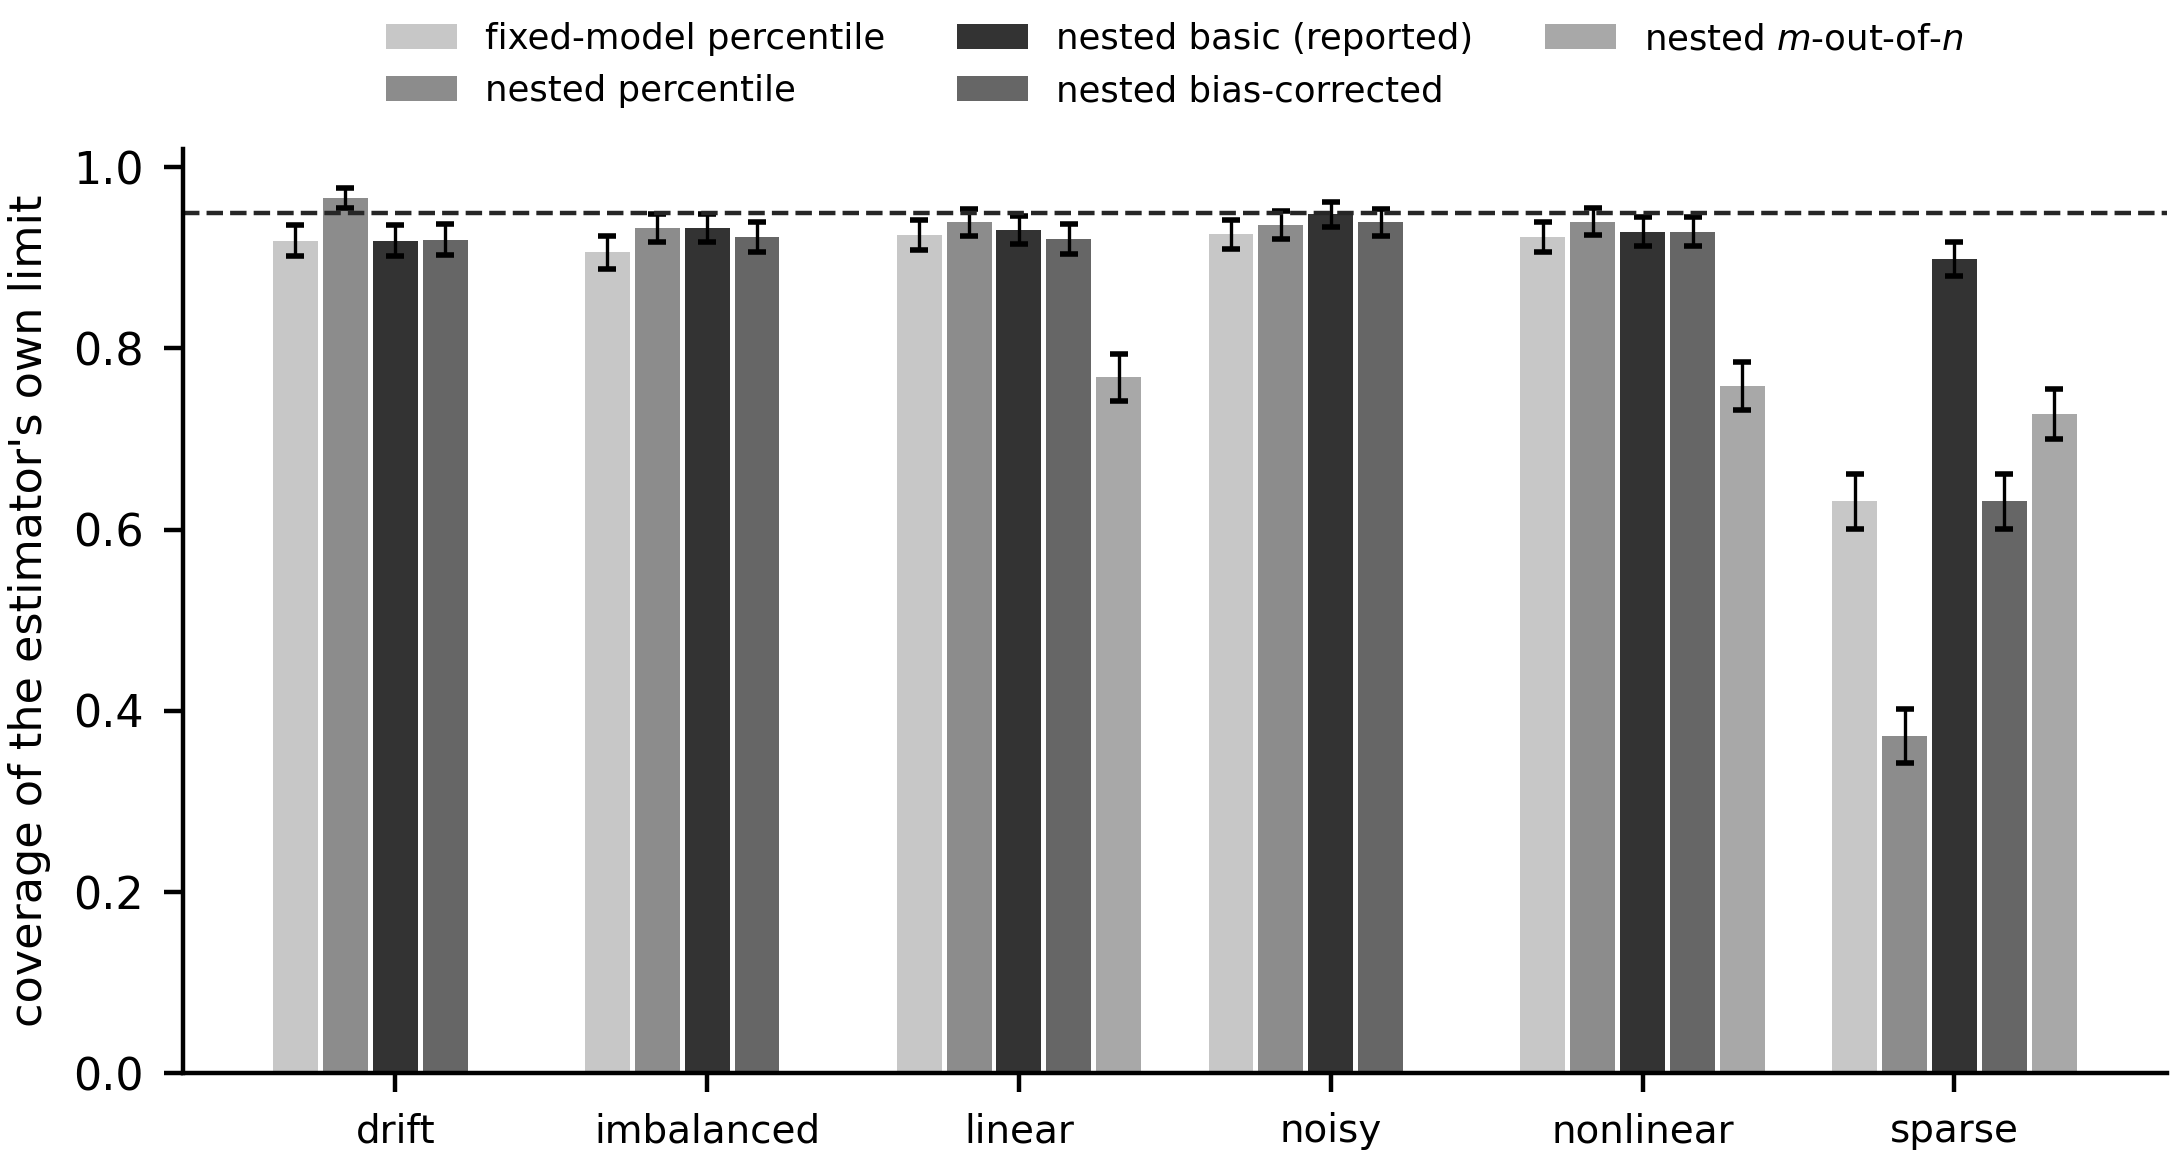
\includegraphics[width=0.9\linewidth]{figS6_coverage.png}
\caption{Coverage of the estimator's own limit in \nWorlds\ simulated worlds,
by interval construction, with Monte Carlo error bars. The dashed line is
nominal. The fixed-model percentile interval is the conventional one; the
nested basic interval is the one this paper reports. The sparse world is where
they disagree by more than a few points, and the nested percentile bar there
is the failure the basic construction repairs.}
\label{fig:coverage}
\end{figure}

\begin{table}[t]
\centering
\small
\resizebox{\ifdim\width>\linewidth\linewidth\else\width\fi}{!}{%%
\begin{tabular}{lrrrrrrrrrr}
\toprule
world & bias vs limit & width (basic) & fixed pct & fixed basic & fixed bc & nested pct & nested basic & nested bc & m-out-of-n & basic vs oracle \\
\midrule
drift & 0.000 & 0.037 & 0.919 & 0.917 & 0.914 & 0.966 & 0.919 & 0.920 & -- & 0.658 \\
imbalanced & $-$0.010 & 0.116 & 0.906 & 0.906 & 0.900 & 0.933 & 0.933 & 0.923 & -- & 0.931 \\
linear & $-$0.002 & 0.060 & 0.925 & 0.931 & 0.915 & 0.939 & 0.931 & 0.921 & 0.768 & 0.931 \\
noisy & $-$0.002 & 0.036 & 0.926 & 0.924 & 0.916 & 0.936 & 0.948 & 0.939 & -- & 0.945 \\
nonlinear & $-$0.002 & 0.044 & 0.923 & 0.923 & 0.924 & 0.940 & 0.929 & 0.929 & 0.758 & 0.930 \\
sparse & $-$0.012 & 0.034 & 0.631 & 0.643 & 0.620 & 0.372 & 0.899 & 0.631 & 0.728 & 0.883 \\
\bottomrule
\end{tabular}%
}
\caption{Coverage of the estimator's own limit $V_{\mathrm{limit}}$ in each simulated world, under seven interval constructions, at the replicate count of Section~\ref{sec:sim}, with the estimator's bias against that limit and the mean width of the interval this paper reports. Nominal is $0.95$; the Monte Carlo standard error on a coverage is \simCoverageSE\ percentage points, so differences below about a point are not differences. An empty cell is a construction not priced on that world. The last column is the reported construction's coverage of $V_{\mathrm{oracle}}$, the Bayes increment, which the estimator is not consistent for on the drifting world.}
\label{tab:sim31}
\end{table}


\begin{table}[t]
\centering
\small
\resizebox{\ifdim\width>\linewidth\linewidth\else\width\fi}{!}{%%
\begin{tabular}{llrrrrlr}
\toprule
n train & K & basic coverage & pct coverage & basic mean width & pct mean width & replicates & coverage se (pp) \\
\midrule
2000 & 20 & 0.887 & 0.887 & 0.085 & 0.085 & 150 & 2.588 \\
2000 & 200 & 0.780 & 0.480 & 0.042 & 0.042 & 150 & 3.382 \\
2000 & 1000 & 0.453 & 0.100 & 0.064 & 0.064 & 150 & 4.065 \\
4000 & 20 & 0.900 & 0.907 & 0.057 & 0.057 & 150 & 2.449 \\
4000 & 200 & 0.907 & 0.500 & 0.031 & 0.031 & 150 & 2.375 \\
4000 & 1000 & 0.507 & 0.080 & 0.047 & 0.047 & 150 & 4.082 \\
8000 & 20 & 0.893 & 0.900 & 0.039 & 0.039 & 150 & 2.520 \\
8000 & 200 & 0.893 & 0.480 & 0.021 & 0.021 & 150 & 2.520 \\
8000 & 1000 & 0.613 & 0.033 & 0.034 & 0.034 & 150 & 3.976 \\
8000 & 3019 & 0.213 & 0.000 & 0.026 & 0.026 & 150 & 3.345 \\
\bottomrule
\end{tabular}%
}
\caption{Sample size and register cardinality varied jointly. Coverage of $V_{\mathrm{limit}}$ and mean interval width for the nested percentile and the nested basic construction. The last row is the cardinality regime of the case study's own register. \emph{How well these are determined.} Every cell is \simGridReps\ replicates, not the \simCoreReps\ of the core experiment, and the coverages here are far from nominal --- so the Monte Carlo standard error of a coverage in this table has a median of \simGridSEMedian\ percentage points and reaches \simGridSEMax, against the \simCoverageSE\ that Section~\ref{sec:simsensitivity} quotes for the core at the nominal rate. It is computed at each cell's own observed rate rather than at the nominal one, and it is a column here rather than a sentence because the differences down this table are read row against row.}
\label{tab:sim31grid}
\end{table}


\begin{table}[t]
\centering
\small
\resizebox{\ifdim\width>\linewidth\linewidth\else\width\fi}{!}{%%
\begin{tabular}{lrrr}
\toprule
world & block multiplier & nested basic & nested pct \\
\midrule
linear & 0.500 & 0.896 & 0.944 \\
linear & 1.000 & 0.920 & 0.908 \\
linear & 2.000 & 0.916 & 0.932 \\
sparse & 0.500 & 0.856 & 0.392 \\
sparse & 1.000 & 0.836 & 0.332 \\
sparse & 2.000 & 0.872 & 0.408 \\
\bottomrule
\end{tabular}%
}
\caption{Three block lengths around $n^{1/3}$: the multiplier column is the factor applied to the rule of thumb, so $0.5$ halves the block and $2$ doubles it. Coverage of $V_{\mathrm{limit}}$, in a run of its own at fewer replicates than Table~\ref{tab:sim31}'s \nSimReps, so its default-block cells are not that table's cells and can differ from them by more than the block effect read down a column here.}
\label{tab:sim31block}
\end{table}


\begin{table}[t]
\centering
\small
\resizebox{\ifdim\width>\linewidth\linewidth\else\width\fi}{!}{%%
\begin{tabular}{llllllllll}
\toprule
family & draws are & K & draws & multiplier & mult., MC upper & empirical & emp., OS upper & Rademacher & per-cell \\
\midrule
decision-curve & degenerate & 248 & 200 & 0.803 & 0.805 & 0.936 & 0.964 & 0.785 & 0.937 \\
decision-curve & degenerate & 1100 & 400 & 0.929 & 0.930 & 0.948 & 0.962 & 0.774 & 0.940 \\
decision-curve & gaussian & 248 & 200 & 0.932 & 0.934 & 0.918 & 0.959 & 0.921 & 0.941 \\
decision-curve & gaussian & 1100 & 400 & 0.932 & 0.937 & 0.920 & 0.954 & 0.926 & 0.945 \\
decision-curve & heavy & 248 & 200 & 0.912 & 0.914 & 0.936 & 0.961 & 0.901 & 0.940 \\
decision-curve & heavy & 1100 & 400 & 0.913 & 0.915 & 0.938 & 0.955 & 0.905 & 0.944 \\
decision-curve & nonzero & 248 & 200 & 0.903 & 0.907 & 0.933 & 0.964 & 0.890 & 0.940 \\
decision-curve & nonzero & 1100 & 400 & 0.921 & 0.921 & 0.943 & 0.957 & 0.916 & 0.946 \\
whole-surface & degenerate & 180 & 400 & 0.924 & 0.924 & 0.945 & 0.966 & 0.920 & 0.946 \\
whole-surface & gaussian & 180 & 400 & 0.943 & 0.945 & 0.937 & 0.959 & 0.936 & 0.946 \\
whole-surface & heavy & 180 & 400 & 0.915 & 0.919 & 0.947 & 0.967 & 0.914 & 0.945 \\
whole-surface & nonzero & 180 & 400 & 0.926 & 0.927 & 0.946 & 0.971 & 0.921 & 0.946 \\
\bottomrule
\end{tabular}%
}
\caption{Family-wise coverage of the max-$t$ band against a known answer, over synthetic families matched to this corpus in size, cross-cell correlation and per-cell excess kurtosis, and spanning draw counts around the one it runs. EVERY ROW IS A FAMILY THE CORPUS RUNS: \textsf{whole-surface} at $K = \nCellsPerPairMedian$ and \nDrawsSurface\ draws is every pair's surface family, \textsf{decision-curve} at $K = \nDcaFamilyModal$ (the grid's rounding of the corpus's modal curve family) and \nDrawsSurface\ draws that family, and the \nDcaFamily-cell row at \nDcaDraws\ draws the case study's own curve family; the draw-count ladder the text quotes is a sensitivity around the first and is not printed here. Nominal is $0.95$; the five middle columns are the five candidate critical values and the last is the control. \emph{The bootstrap here is ideal} --- the draws come from the sampling distribution itself --- so every coverage in this table is an upper bound on what the real procedure attains, and the control says why: \emph{per-cell} is the basic interval the band is built from, on the same draws, and it is short of nominal before any multiplicity correction is applied. \emph{Regimes.} \textsf{gaussian} is the case the multiplier bootstrap is derived for; \textsf{heavy} carries this corpus's measured tails; \textsf{degenerate} adds the cells whose net-benefit difference is zero by arithmetic, which the corpus's decision-curve families contain and its surface families do not; \textsf{nonzero} is heavy with a fixed heterogeneous non-zero truth, the regime under which a cell can be resolved correctly and a region label is actually being asked to hold. Every cell is \nBandCoverageReps\ replicates, so no coverage here is determined worse than \bandCoverageSEMax.}
\label{tab:bandcov}
\end{table}


\begin{table}[t]
\centering
\small
\resizebox{\ifdim\width>\linewidth\linewidth\else\width\fi}{!}{%%
\begin{tabular}{lllrlrrrrrrr}
\toprule
world & n train & K & K / n & replicates & coverage at c = 1 & se & c & c lo & c hi & c monotone & c log-linear \\
\midrule
linear & 180000 & 200 & 0.001 & 500 & 0.882 & 0.014 & 1.352 & 1.174 & 1.482 & 1.177 & 1.000 \\
linear & 8000 & 20 & 0.003 & 500 & 0.916 & 0.012 & 1.154 & 1.073 & 1.307 & 1.177 & 1.000 \\
linear & 4000 & 20 & 0.005 & 500 & 0.898 & 0.014 & 1.219 & 1.101 & 1.313 & 1.177 & 1.056 \\
linear & 2000 & 20 & 0.010 & 500 & 0.924 & 0.012 & 1.108 & 1.024 & 1.228 & 1.177 & 1.134 \\
linear & 50000 & 625 & 0.013 & 498 & 0.902 & 0.013 & 1.296 & 1.135 & 1.689 & 1.177 & 1.160 \\
linear & 8000 & 100 & 0.013 & 500 & 0.936 & 0.011 & 1.096 & 0.960 & 1.203 & 1.177 & 1.160 \\
sparse & 8000 & 100 & 0.013 & 500 & 0.892 & 0.014 & 1.317 & 1.220 & 1.453 & 1.177 & 1.160 \\
linear & 2000 & 25 & 0.013 & 500 & 0.908 & 0.013 & 1.188 & 1.072 & 1.277 & 1.177 & 1.160 \\
linear & 750 & 10 & 0.013 & 500 & 0.920 & 0.012 & 1.117 & 1.029 & 1.207 & 1.177 & 1.168 \\
linear & 4000 & 100 & 0.025 & 500 & 0.896 & 0.014 & 1.179 & 1.087 & 1.296 & 1.177 & 1.245 \\
linear & 8000 & 200 & 0.025 & 499 & 0.932 & 0.011 & 1.093 & 0.985 & 1.264 & 1.177 & 1.245 \\
sparse & 4000 & 200 & 0.050 & 500 & 0.884 & 0.014 & 1.182 & 1.131 & 1.299 & 1.177 & 1.337 \\
linear & 2000 & 100 & 0.050 & 500 & 0.912 & 0.013 & 1.234 & 1.055 & 1.326 & 1.177 & 1.337 \\
linear & 4000 & 200 & 0.050 & 500 & 0.888 & 0.014 & 1.195 & 1.119 & 1.337 & 1.177 & 1.337 \\
linear & 8000 & 400 & 0.050 & 500 & 0.884 & 0.014 & 1.152 & 1.104 & 1.226 & 1.177 & 1.337 \\
linear & 750 & 38 & 0.051 & 500 & 0.926 & 0.012 & 1.103 & 0.989 & 1.259 & 1.177 & 1.338 \\
sparse & 2000 & 200 & 0.100 & 500 & 0.836 & 0.017 & 1.333 & 1.224 & 1.372 & 1.310 & 1.435 \\
linear & 500 & 50 & 0.100 & 500 & 0.874 & 0.015 & 1.250 & 1.141 & 1.460 & 1.310 & 1.435 \\
linear & 4000 & 400 & 0.100 & 499 & 0.796 & 0.018 & 1.287 & 1.221 & 1.399 & 1.310 & 1.435 \\
linear & 2000 & 200 & 0.100 & 500 & 0.844 & 0.016 & 1.316 & 1.253 & 1.417 & 1.310 & 1.435 \\
linear & 8000 & 1000 & 0.125 & 496 & 0.655 & 0.021 & 1.526 & 1.417 & 1.600 & 1.441 & 1.468 \\
linear & 2000 & 250 & 0.125 & 500 & 0.792 & 0.018 & 1.404 & 1.284 & 1.485 & 1.441 & 1.468 \\
linear & 750 & 94 & 0.125 & 500 & 0.872 & 0.015 & 1.310 & 1.154 & 1.396 & 1.441 & 1.468 \\
linear & 2000 & 400 & 0.200 & 500 & 0.758 & 0.019 & 1.562 & 1.398 & 1.670 & 1.562 & 1.540 \\
sparse & 4000 & 1000 & 0.250 & 498 & 0.460 & 0.022 & 1.716 & 1.672 & 1.849 & 1.727 & 1.575 \\
linear & 4000 & 1000 & 0.250 & 500 & 0.520 & 0.022 & 1.739 & 1.632 & 1.805 & 1.727 & 1.575 \\
linear & 8000 & 3019 & 0.377 & 488 & 0.305 & 0.021 & 1.881 & 1.804 & 1.988 & 1.791 & 1.643 \\
linear & 500 & 200 & 0.400 & 500 & 0.760 & 0.019 & 1.450 & 1.353 & 1.656 & 1.791 & 1.653 \\
linear & 2000 & 1000 & 0.500 & 500 & 0.462 & 0.022 & 1.869 & 1.788 & 2.024 & 1.869 & 1.691 \\
\bottomrule
\end{tabular}%
}
\caption{The coverage calibration. For each cell of the $(n, K)$ plane: the coverage the reported interval actually attains, and the factor $c$ by which it must be widened to attain the nominal level, with the Monte Carlo interval of that factor. $c$ is the $0.95$ quantile of the studentised error and is computed, not searched for. THIS CALIBRATION IS DERIVED AND REPORTED, NOT APPLIED: it is fitted to restore POINTWISE coverage on this plane, the article reports the labels under it only as a sensitivity, and no band in the article is widened by it. Section~\ref{sec:simband} measures the operative critical value at about its level on the family matched to this design under an ideal bootstrap, which bounds the critical value's contribution to coverage and not the resampling's; the pointwise shortfall this plane measures (Section~\ref{sec:simsensitivity}) is the part that bound leaves open. `c monotone' is the monotone regression that would be used if it were; `c log-linear' is the parametric fit whose slope Section~\ref{app:curves} quotes, printed beside it because it sits below the measured factor at small ratios and would under-correct there.}
\label{tab:plane}
\end{table}



\section{What the corpus does and does not have in common}
\label{app:construct}
%  Moved from the article (30_design.tex, \subsection{What the corpus does and does not have in common}) in the IJF retarget, PLAN-IJF.md
%  Task 2.1; the article keeps a pointer paragraph.
The corpus is \nLogs\ public logs spanning \nDomains\ domains, including the
further ITSM logs the literature uses \citep{steeman2013bpic,amaral2018incident},
and it is heterogeneous: the registers are a configuration item, a caller, a
product, a vendor, a diagnosis and a legal article, and the targets mean
different things in a bank's incident queue, a hospital's admissions and a
municipality's permits. Table~\ref{tab:construct} names, for every pair, the
domain, the field playing each role, the target's interpretation and the
construct threat that pair carries --- a diagnosis code is admitted by a
cardinality-and-reuse rule and is not a configuration management database.
This is therefore a \emph{benchmark of specification sensitivity across
heterogeneous forecasting problems}, not a replication of one finding on
several organisations, and two disciplines follow: no effect magnitude is
averaged across domains as though it estimated one universal register value,
and the \nITSMPairs\ ITSM-like pairs, the closest family to the case study,
are analysed as a group as well, with every headline corpus statistic
reported on both populations in Section~\ref{sec:family}.


\section{Against specification-curve analysis as practised}
\label{app:sca}
%  Moved from the article (40_multilog.tex, \subsection{Against specification-curve analysis as practised}) in the IJF retarget, PLAN-IJF.md
%  Task 2.1; the article keeps a pointer paragraph.
The closest existing practice is specification-curve analysis
\citep{simonsohn2020specification}: enumerate the reasonable specifications,
plot the curve, and test it against a sharp null by permutation.
Table~\ref{tab:sca} runs it unchanged on \emph{every} admitted pair ---
\nScaPairs\ of them, \nScaPerms\ permutations of a declared
\nScaCells-cell sub-surface, under budgets Table~\ref{tab:sca}
declares --- beside the region label of the pair's whole inference family,
which contains that sub-surface (Table~\ref{tab:sca}'s caption says so), which makes
``how often do the two verdicts part company'' a measurement rather than an
illustration.

\textbf{They part company on \nScaDisagree\ of the \nScaPairs\ pairs}, close
to half: the permutation test rejects the sharp null --- the surface is
decisively unlike one with no signal --- and the same cells contain
increments of \emph{both} signs, so a reader given only the test would
conclude that the register matters and have no way to learn that whether it
helps or hurts depends on choices nobody told them about. On
\nScaAgreeNull\ of the \nScaPairs\ pairs neither resolves and the cheaper
metric suffices. And a specification curve is a statement about the
cells it enumerates: on \nScaSubSurfaceDisagree\ of the \nScaPairs\ pairs
--- \scaSubSurfacePair\ --- every cell of the sub-surface has one sign while
the \emph{full} surface is \scaSubSurfaceRegion, and nothing is wrong with
either, because they are claims about different sets; without a declared
denominator and a simultaneous band a curve cannot distinguish ``the sign
holds'' from ``the sign holds on the cells that were drawn''.

Neither subsumes the other. The permutation test answers \emph{is there
anything here}, costs one refit per permutation per cell and needs no band;
the region answers \emph{may I quote a sign}, costs a nested bootstrap, and is
what a reader deciding whether to act needs. This paper's contribution is the
second, and the first should be reported beside it.



\section{What the case study says to a configuration management programme}
\label{app:programmeread}
%  Moved from the article (50_cmdb.tex, \subsection{What this says to a configuration management programme}) in the IJF retarget, PLAN-IJF.md
%  Task 2.1; the article keeps a pointer paragraph.
This subsection is the reading a service-management audience will want, stated
in the estate's own vocabulary. It is a reading of \emph{one} estate on
\emph{one} public log and it is offered as one; Section~\ref{sec:lim} says
what a second would need.

\paragraph{The three moments, in service-desk terms}
The prediction is: \emph{will this case be reassigned to another group before
it is resolved?} The register is the affected configuration item, the free
field the assignment group --- the routing queue, recorded without a
configuration management database and the field the register has to beat ---
the intake block what the desk records when the case arrives, and the
knowledge reference a pointer to a knowledge-base article whose availability
at the moment of decision is exactly what Section~\ref{sec:quality} cannot
settle. $\tau_0$ is \emph{an interaction is logged}: every call is in scope,
\nTauZero\ of them. $\tau_1$ is the same moment restricted to the calls that
will escalate. $\tau_2$ is \emph{an incident record is created}: \nTauTwo\
cases, \nTauTwoUnmatched\ of them with no interaction record. Read down
Table~\ref{tab:tau} and the register's worth falls from \VtauZero\ AUC to
\VtauOne\ to \VTtwoGroup\ once the routing queue is in the baseline, and to
\VTtwoKnow\ --- not resolvably different from zero --- once the knowledge
reference is admitted too. A programme that justifies the register on a
first-touch number and deploys the model at incident creation is quoting the
top of a ladder and standing on the bottom of it;
Section~\ref{sec:nbregret} prices that at \promisedPerThousand\ true
positives promised per thousand cases against \deliveredPerThousand\
delivered.

\paragraph{Which layer of the register pays}
A programme does not choose whether to have a configuration management
database; it chooses how much of one to populate and maintain, which is a
choice among \emph{layers}. On the registered cohort and handover rule ---
\layerLadderN\ cases, one-hot logistic regression at the temporal holdout,
against the intake block at base AUC \layerBaseHandover\ --- the item's
\emph{type} (\nLayerTypeLevels\ values) is worth \layerTypeHandover\ AUC over
intake, its \emph{subtype} (\nLayerSubtypeLevels) \layerSubtypeHandover, and
the item itself \layerItemHandover, adding \layerItemMarginalHandover\ once
the subtype is in the model; that ladder is on a different cohort and target
from Table~\ref{tab:tau} and does not reconcile with it arithmetically
(Supplement~\ref{app:layers}). \textbf{The coarse layers are not free, and
the finest layer is not redundant}: \layerTypeSharePctHandover\ of what the
item is worth is reachable from a thirteen-value type field, and the item
still adds once the subtype is known. On the duration target the ladder
gives \layerTypeDuration, \layerSubtypeDuration\ and \layerItemDuration, with
\layerItemMarginalDuration\ marginal and the type reaching
\layerTypeSharePctDuration, so the split between the layers is a property of
the target and not of the register; Supplement~\ref{app:layers} carries two
further logs on which every coarse layer is worth essentially nothing while
the finest one is not. Nothing here prices what a layer costs to populate or
to keep accurate.

\paragraph{What would have to change for the answer to move}
Three things, in the order a programme could act on them. A
\emph{timestamped field history}: the knowledge reference decides this
estate's answer and its admissibility is settled here by probability, and a
register that records when each value was written turns
Section~\ref{sec:quality}'s tipping point into a measurement. A
\emph{complete population at the forecast origin}: \nTauTwoUnmatched\ incidents
have no interaction record, so the $\tau_1$-to-$\tau_2$ step is an
information step only on the cases that have both. And a \emph{target the
desk actually acts on}: the register's sign changes with the target on this
log (Section~\ref{sec:cohort}), and a programme evaluating a register against
a generic handover rule is answering a question nobody asked it.



\section{The absorption ladder, and why the ratio is secondary}
\label{app:absorption}
%  Moved from the article (50_cmdb.tex, \subsection{The absorption, and why the ratio is secondary}) in the IJF retarget, PLAN-IJF.md
%  Task 2.1; the article keeps a pointer paragraph.
The quantity a report of this kind usually leads with is the \emph{relative}
reduction $R$: the share of the register's apparent value that a single free
field absorbs. The absolute absorption $D = V(f \mid B_0) - V(f \mid B_1)$ is
reported first, with its own interval, and $R$ second with a Fieller set and
the set's kind. On this estate at the reference cell $D$ is \Dabs\ [\DabsLo,
\DabsHi] and $R$ is \Rref\ with a \RrefKind\ Fieller set; \nFiellerUnboundedCase\
of the \nFiellerCase\ reductions this ladder produces have a non-bounded set,
because the denominator is resolvably positive at every rung, which across the
corpus is not so (Section~\ref{sec:reduction}). The full ladder is
Table~\ref{tab:absorption}.


\section{Threats to validity: the internal-validity detail the article summarises}
\label{app:threats}
%%  Moved from the article's Threats to validity (80_limits.tex) in the IJF
%%  retarget, PLAN-IJF.md Task 2.1; the article keeps each paragraph's
%%  verdict and points here for the argument.

\paragraph{What the band's coverage does and does not establish --- the three qualifications}
The measurement switches the resampling off, so it
bounds the critical value's contribution and not the bootstrap's: the
pointwise interval underneath is governed by $K/n$ and undercovers where
this corpus lives (Section~\ref{sec:simsensitivity}), and the $(n, K)$
calibration that would widen it is reported as a sensitivity and not
applied, because it is fitted pointwise, applied simultaneously and
measurably misspecified. The level is bought with width:
\nResolvedLostToEmp\ cells the multiplier would have resolved are unresolved
here, and \nUnresolvedPairs\ pairs resolve nothing. And the decision-curve
families carry cells that are zero by arithmetic, which a declared rule
excludes from the family before the quantile is taken
(Section~\ref{sec:dcabands}). The decision-curve region of that section is
the exception to the first sentence of this paragraph's verdict: its family's
empirical quantile covers \covEmpHeavyCaseAtDesign\ on a matched family that
reproduces the corpus's estimator ratio at \ratioSynthDca\ against
\ratioCorpusDca, so that label rests on a critical value about a point short
of its level.

\paragraph{Internal --- two mechanisms this evidence retires}
A multinomial resample holds about $1 - e^{-1}$ of a high-cardinality
register's levels, which is the natural explanation of a displaced bootstrap
distribution. Under weights every row has positive weight in every draw and
the level share is \levelShareWeighted\ against \levelShareMult\ --- the
mechanism is gone by construction --- and the displacement's median moves
only from \dispMedianMult\ to \dispMedianWeighted\ (Section~\ref{sec:boot}).
What the change does remove is a defect the mechanism genuinely caused:
cells a draw drops entirely, which get no band at all and were counted as
\emph{unresolved} beside cells that were banded and straddled zero ---
\nUnbandableSameDesign\ under the multinomial scheme on this design,
\nUnbandableCells\ under weights. And the draw count is not what governs the
multiplier's coverage: on families matched to this design it is
\covMultBootOneFifty\ at \nBootOneFifty\ draws, \covMultBootFourHundred\ at
\nBootFourHundred\ and \covMultBootOneThousand\ at \nBootOneThousand\ ---
it plateaus --- while the empirical quantile's coverage is what rises with
$B$, from \covEmpBootThirtyThree\ at \nBootThirtyThree\ draws to
\covEmpBootFourHundred\ at \nBootFourHundred. A mechanism can be removed
completely and leave its supposed consequence standing, which is a caution
about every explanation of a resampling artefact offered without the
counterfactual, including the two here.

\paragraph{Internal --- further assumptions, named, and one of them
measured}
The split point is fixed within a draw, so split-position uncertainty is
outside every interval here. A second sort is undeclared and is not repaired:
the register-quality mechanisms cut a cumulative-count curve inside a group
of tied identities, so \emph{which} identities a degradation removes rests on
an order nothing pins; the affected quantity is the quality axis and not the
increment at the reference cell, and repairing it moves every number on that
axis, which is why it is recorded here and why
Supplement~\ref{app:standard}'s tie-break item ranges over every sort a
procedure cuts on. The moving-block construction needs stationarity and
mixing that an event log is not guaranteed to have, and the same assumption
makes Definition~\ref{def:estimand}'s population limit well defined under a
temporal split. Stationarity is measured and does not hold everywhere:
cutting each pair's test half into \nDriftBlocks\ consecutive blocks and
reading the spread of the increment against a null that re-partitions the
same rows at random, \nDrifts\ of \nDriftPairs\ pairs sit in the upper tail
of that null at $\alpha = 0.05$, \nDriftSignVaries\ carry both signs between
blocks of one test half, and only \nDriftTrend\ shows a monotone trend, so
this is heterogeneity and not decay (Supplement~\ref{app:drift}). On those
pairs the interval and the band understate what a reader would see on a
different stretch of the same log, by an amount this design cannot sign;
time is not a declared axis of $\mathcal{S}$. Mixing is not tested. The
band's family-wise coverage is asymptotic, the block length is a convention,
$\lceil n^{1/3}\rceil$, which moves coverage by up to
\coverageBlockSpreadMax\ within a world, and the $(n, K)$ calibration of
Supplement~\ref{app:calibration} corrects the studentised statistic's
\emph{scale} and not the shape of the maximum's distribution and is
measurably misspecified ($\log n$ enters at $t = \planeNdependenceT$). A
reader who rejects any of these should rely on the objects that need no
band: the point estimates, the decomposition, the disagreement rates and the
regret comparison.



%%  ROUND TWENTY-SEVEN.  The reporting standard moved here from Section 9 in
%%  the length pass; the two that follow it are a different repair.
%%  BOTH DOCUMENTS PROMISED THE CORRECTION REGISTER AND THE PILOT and neither
%%  compiled them.  The article's front matter (Section 1) and this
%%  supplement's own abstract each list "the correction register" among the
%%  supplement's contents, and the archive description cites it by name --
%%  while `app_corrections' and `app_pilot' were reachable only from
%%  `_appendix_block.tex', which no built document includes.  A promise a
%%  referee can check in one click is worth more attention than a page count.
\section{A reporting standard, and software}
\label{app:standard}
%%  ROUND TWENTY-SEVEN.  Moved from Section 9 for length, unchanged.
%%  The prescription itself stays in the article as a paragraph at the
%%  end of Section 4; what moved here is the apparatus -- the six-step
%%  recipe, the package, the worked example and the practice pilot.

\subsection{The minimum reportable form}

The apparatus of Sections~\ref{sec:surface} and~\ref{sec:inference} implies a
reporting standard short enough to state in full. An incremental-performance claim is
reportable when it carries: \textbf{the design space}, as an enumerable
declaration of which learners, encodings, targets, splits, forecast origins,
quality mechanisms, baselines, metrics and operating points are admissible,
why anything defensible was left out, and \emph{the measure placed on those
levels}; \textbf{the denominator}, as a count a reader can reproduce from the
axis levels --- declared cells, computed cells, and the cells any inference
actually rests on, which need not be the same set; \textbf{the absolute
increments} at every rung of the baseline ladder, in the metric's own units,
with intervals from a resampling scheme that refits the model; \textbf{the
sensitivity decomposition}, with the total higher-order share reported as
$1 - \sum_i S_i$ and not as any per-axis difference; \textbf{the resolution
region and $\rho$}, under a band whose family is the set the label ranges
over; and \textbf{the ratio $R$ last if at all}, with a Fieller set and the
set's kind, never where the denominator is not resolvably positive.

\textbf{Five further items, each of which this study got wrong before it got
right.} \emph{The tie-break rule} on \emph{every} sort a procedure cuts on,
and not only on the sort that produces the split: an undeclared one there
moved this study's own case-study increment by
\tiebreakShiftPct\ of its magnitude and left it ranging over
\tiebreakRangeSharePct\ of that magnitude under random tie orders
(Section~\ref{sec:cohort}). The item is stated at that width because the
narrow version of it missed a second instance in this same study: the
register-quality mechanisms cut a cumulative-count curve inside a group of
tied identities, so \emph{which} identities a degradation removes also rests
on an order nothing pins. That one is recorded rather than
repaired --- repairing it moves every number on the quality axis --- and
\reproduceguide\ in the archive records it. \emph{Which halves a quality
counterfactual is applied to}, and which half its parameters are estimated
from (Section~\ref{sec:quality}). \emph{A minimal practically important
difference}, declared before any disagreement rate is computed and in the
units of one named instrument (Section~\ref{sec:results-regret}).
\emph{Which axes are resampling rather than analyst latitude}, so that a
decomposition is not read as specification sensitivity when it is sampling
variability (Section~\ref{sec:sobol}). And \emph{the draw count and the
\emph{effective} draw count} behind every band, together with whatever is
known about the coverage those draws buy --- because a band reported without
them invites a reader to assume its nominal level, which
Section~\ref{sec:simband} shows is not attained here. Nothing in the list is
expensive once the surface exists, and the surface is a factorial over
declarations the analyst has already made implicitly.

\paragraph{Applying it to a field of your own, in six steps}
\textbf{One}, name the roles: the field $f$ whose worth is in question, the
cheap field $g$ it must beat, and the intake block $B_0$ available at the
forecast origin. \textbf{Two}, declare the space: list every level of every
axis you would have accepted \emph{before} seeing a result, and the measure
over them. \textbf{Three}, compute the surface --- one call, one cell per
specification --- and audit the denominator by multiplying the level counts
and comparing with the row count. \textbf{Four}, decompose it with the
resampling axes held as an error stratum, and report the analyst-choice shares
as primary. \textbf{Five}, band it over the family your claim ranges over,
not over one cell, and state the draw count and what coverage those draws
attain. \textbf{Six}, report the region and $\rho$ with the triple of counts
they rest on, and refuse a direction below your declared minimum resolved
share. The package below performs steps three to six from a tidy frame.

\subsection{\Pkgname}
\label{sec:tool}

The standard ships as \pkgname\ \citep{fieldvalue}, which computes the surface from a
data frame, a feature name and a dictionary of baselines. Its notable
property is a refusal: \texttt{Surface} raises rather than returning a
scalar, \texttt{Surface.report()} emits the form above, and
\texttt{Surface.at(...)} returns one cell only if the caller names every
axis. Version \fvVersion\ implements
Sections~\ref{sec:sobol}--\ref{sec:regionsdef} of the article and
Section~\ref{app:regretfull} here as four functions of a surface
--- \texttt{decompose}, \texttt{regions}, \texttt{robustness} and, for the
robustness check of Section~\ref{sec:regretdef}, \texttt{regret} --- each
taking a tidy frame rather than this package's own object, so they
apply to a surface computed by some other pipeline. It carries \nTests\ tests
and is an \emph{independent implementation}: the analysis scripts and the
package compute the same quantities from the same definitions in different
code, neither written against the other, and on this corpus they agree on
\nAgreeQuantities\ of \nAgreeQuantities\ quantities to \agreeTolerance.

\subsection{Beyond process logs, and beyond this paper's claims}
\label{sec:worked}

The standard is not about event logs and not about configuration databases.
Section~\ref{app:worked} runs it on UCI Adult, where the expensive field is
\texttt{occupation} and the cheap ones come with the sampling frame: over
\exCells\ cells the reduction runs \exRmin\ to \exRmax; the baseline and the
metric carry the same share of the variance to three figures,
\exSbaselinePct\ and \exSmetricPct\ --- a coincidence rather than a copy
error, as the fourth figure shows: \exSbaselineFine\ against \exSmetricFine\
--- against \exSpopulationPct\ for the
register population; and a one-number report misstates the sign for a mean
\exMisreportPct\ of the other cells. \texttt{examples/worked\_example.py}
produces all of it in \exampleLines\ statements against the package's public
interface.

\paragraph{How the surface is reported today}
\label{sec:practice}
Whether the axes this paper varies are varied in published work deserves a
systematic review, and we did not conduct one: a prevalence pilot with one
adjudicator --- assisted by a large-language-model assistant, which the
generative-AI declaration accompanying the article (on its title page) names
with version and dates --- was run on a convenience frame, is \emph{not}
reported in the article because that adjudicator and a screen of measured
sensitivity \auditSens\ can generate a hypothesis about practice and cannot
test one; Section~\ref{app:pilot} gives it in full, and the archive carries its
frame, sample, codes and adjudications, with the evidence dossiers rebuilt
from the retrieved full texts by script. The paper's argument does not need
it.

\section{The correction register}
\label{app:corrections}

This project keeps a correction register. Earlier versions of this work
carried it in the main text; a referee of an earlier version observed that
scientific transparency should be visible in the design and the supplement
rather than repeatedly asserted, and that is right, so it is here.

\refereelog\ carries every objection recorded
against this work --- from referees of earlier versions and from the
authors' own adversarial reads --- each with its disposition and with the
corrections it produced named. What follows is the register grouped by \emph{class}, because the
classes are more useful than the incidents: they say what kind of mistake this
apparatus is prone to. Identifiers run in the order the corrections were made,
across all twenty rounds; three of the low numbers never entered the register
and the classes below are therefore not a contiguous range, which is a fact
about the numbering and not a missing entry.

\paragraph{Class A --- a control that could not fail}
Four corrections (C1, C2, C8, C16) are nulls or searches drawn at the wrong
level, swept over the wrong range, or given fresh noise inside a comparison
that assumed determinism. A null that cannot fail is worse than no null,
because it is reported as evidence. The most recent, C16, is in
Section~\ref{app:props}: the axis non-redundancy search drew fresh noise
inside each cell evaluation, so two evaluations of the same cell disagreed and
the search found almost nothing.

\paragraph{Class B --- a quantity whose sign was set by a tie-break}
Two corrections (C4, C7) concern an operational factor computed at a fixed
review capacity, where $93.1\%$ of what the naive baseline nominated came from
a single tied block and reordering rows inside that block moved the arm from
$-26$ to $+608$. A quantity whose sign is set by a tie-break is not a
measurement. Section~\ref{sec:dca} is built on net benefit, which admits or
excludes a whole tied block at a threshold and never breaks one.

\paragraph{Class C --- every literal correct, the relation between them
false}
Five corrections (C9, C10, C12, C13, C14) are sentences in which each printed
number was right and the claim asserted about them was not: an extremum that
was the worst of the points the table happened to name; a count reported as a
contiguous run; a range ``across the operating range'' that was a range across
five named points; a universal ``if and only if'' whose necessity direction is
only existential (Section~\ref{sec:props}); and --- the one that mattered most
--- a headline spread that was inflated by an intercept-only baseline no
analyst would build, while a later section of the same manuscript said so and
the abstract did not. This class is the reason
Section~\ref{sec:regionsdef} excludes the intercept-only rung by definition and
the reason every number in this document is a generated macro rather than a
typed literal.

\paragraph{Class D --- evidence one download away}
One correction (C11): an earlier version reported that it could not establish
whether the knowledge-article reference was available at incident creation,
named the file that would settle where the field comes from, and did not
obtain it. Obtaining it changed the headline. Section~\ref{sec:cmdb} now
reports the register at three forecast origins (Table~\ref{tab:tau}) rather
than choosing one, because obtaining the file settled where the field is
written and not when.

\paragraph{Class E --- a claim about the world that our own coder could not
support}
One correction (C15), and it is the largest. An earlier version reported that
\emph{not one} of twenty audited papers reports the increment across a range
of operating points. The rebuilt pilot of Section~\ref{sec:practice}
adjudicates the papers the mechanical screen \emph{rejected} as well as the
ones it accepted, measures the screen's sensitivity at \auditSens, and finds
eligible papers that do report the increment across a range of operating
points --- one of them at four values of $k$ in a top-$k$ evaluation. The
earlier ``not one'' was a property of a coder that finds fewer than half of
the eligible papers, not a property of the literature. The corrected estimate
is \auditRangeThresholdPct\ with an interval that includes it.

\paragraph{Class F --- internal inconsistency}
Four corrections (C17, C18, C19, C22) are places where an earlier manuscript
disagreed with itself: an instrument count that treated two thresholds of one
instrument as two instruments; a reference reduction quoted as
$43.7\%$ in the text and $35.0\%$ in a table without the change of
specification being made clear; and a section that said a withdrawn
instrument was retained in a table that did not contain it. The generated-macro
discipline of Section~\ref{app:verifier} makes this class structurally
impossible rather than merely unlikely --- and does not make it impossible
when the same wrong quantity is computed twice from the same wrong expression,
which is C22. Correcting the pilot's frame size in the facts and not in the
PRISMA flow left Section~\ref{sec:practice} reading
\nAuditFrame\ and Table~\ref{tab:prisma} reading two orders of magnitude more, four pages apart,
\emph{after} the error had been found and written up. The frame is computed
once now, before both consumers, and the verifier checks every row of the flow
that the prose also quotes.

\paragraph{Class G --- an estimand that was not the one being estimated}
One correction (C20), found in round nineteen and the reason
Section~\ref{app:noisy} exists. The simulation of Section~\ref{sec:sim}
computed both estimands by enumerating the data generator's cells, which in
the noisy world carry the register's \emph{true} value while the estimator
only ever observes a value replaced by a uniform draw with probability
\simNoiseRate. Coverage was therefore measured against a population the
estimator does not sample from, and came out at \coverageNoisyBefore\ with an
apparent bias of \biasNoisyBefore. Both were artefacts. The correction is
exact marginalisation of the noise; the estimator's mean was
\meanNoisyEstimate\ before and after.

This class is worth separating from Class F because nothing in the
generated-macro discipline could have caught it: every number was internally
consistent, correctly computed, and correctly printed. What was wrong was the
\emph{definition} of the quantity two of them referred to. It was found by
constructing two experiments that could each have confirmed the comfortable
reading --- that the method simply fails in that world --- and having both
refuse to. That is the only mechanism in this project that has ever caught an
error of this class, and it is not automatable.

\paragraph{Class H --- a statistic aggregated over the wrong index set}
One correction (C21). The literature pilot's frame size summed a stratum-size
column over the \emph{rows} of the sample rather than over its distinct
strata, and a stratum's size is carried on every row of that stratum. The
quantity computed was $\sum_h N_h n_h$ and the quantity intended was
$\sum_h N_h$, so a frame of \nAuditFrame\ records was reported as one two
orders of magnitude larger. Every input was correct; the arithmetic was
correct; the group-by was wrong.

The correction changed what the pilot \emph{is} and not only how large it
sounds. With the true frame in view it is immediate that the design weight is
\auditMaxWeight\ in every stratum, that the enumeration stopped short of its
declared budget of \nAuditTarget, and that the pilot is therefore a census of
what one index returned rather than a probability sample of a literature ---
which Section~\ref{sec:practice} now says, with the additional limit that the
frame's coverage of the field is unmeasured.

The guard is a re-derivation rather than a recount: the verifier computes the
frame from the sample by grouping, and refuses a manuscript in which a frame
is smaller than the sample it contains, or differs from it while every design
weight is one. A checker that recomputed the same aggregation would have
agreed with the error.

\paragraph{Class I --- an inferential object whose denominator was not the
one the claim quantified over}
Two corrections (C26, C28), and they are the same mistake in two places. A
region label such as \emph{uniformly beneficial} ranges over every admissible
cell of a surface, and an earlier version supported it with max-$t$ bands
whose family was the five scalar instruments \emph{at one cell}; the family
was two orders of magnitude smaller than the claim. Widening it to the whole
surface raises the critical value from \maxTWithinMedian\ to
\maxTSurfaceMedian\ at the median pair and changes the region label on
\nRegionChangedByFamily\ of \nPairs\ pairs --- and more at the cell level,
where a region label's coarseness no longer hides it and the wider family
unresolves cells throughout. Section~\ref{sec:simbands} now
declares four interval objects by name so a table cannot print one and be read
as the other. The same class covers the
pilot's Wilson intervals (C28): a binomial interval was put around a ratio of
two weighted totals through a fractional ``effective sample size'', and none
of the five resulting intervals contains its design-based counterpart.

The general form is worth stating because it is not a coding error and no
checker in this repository would have caught it: \textbf{an interval is only
as good as the correspondence between the family it controls and the sentence
it is used to license}, and that correspondence is a judgement about English,
not a property of the arithmetic.

\paragraph{Class J --- a quantity assembled from units that do not add}
Two corrections (C25, C27). The first: an earlier version reported the largest
per-axis difference $\max_i(S_{T_i} - S_i)$ and described it as the share of
variance carried by interactions. Those differences overlap across axes ---
a two-way component appears in the total effect of both of its axes --- so
their maximum is neither their sum nor their union, and the total higher-order
share is $1 - \sum_i S_i$, which on this corpus is \interactionTotalPct\
against the \largestInvolvementPct\ that was printed. The second: expected
regret was averaged over an admissible set spanning five scalar instruments
and reported as a single percentage ``in the metric's own units''. There is no
such unit once AUC and Brier skill are inside one average.
Section~\ref{sec:rules} now reports regret inside one instrument at a time,
and Section~\ref{sec:nbregret} reports a common-utility version on calibrated
net benefit, which is a scale on which averaging is defined.

\paragraph{Class K --- a theorem stated wider than its proof, and wider than
the truth}
Two corrections (C23, C24). The necessity direction of the rank-invariance
proposition quantified over every non-rank-based instrument and was supported
by one stored configuration for five named instruments under one map. Repairing
the proof also refuted the claim: what invariance of the \emph{reduction}
requires is that the recalibration act \emph{affinely} on the instrument, not
that it leave it fixed, and Section~\ref{sec:props} exhibits a
non-rank-based instrument whose reduction is invariant. The word
\emph{exactly} was wrong, not merely unproved. C24 withdraws the axis
non-redundancy search entirely: its answer moved with an arbitrary tolerance,
no claim depended on it, and removing it was cheaper than repairing it.

\paragraph{Class L --- a number the design cannot produce, and a word the
design does not license}
Two corrections (C29, C30). An earlier version printed raw and Holm-adjusted
bootstrap $p$-values of $0.000$ from 200 draws; no finite bootstrap can
produce zero,
and Section~\ref{sec:planned} now uses the plus-one estimator with the
smallest attainable value stated beside it. And the five contrasts were called
\emph{confirmatory} when they had been fixed after eighteen rounds of analysis
on the same data; they are \emph{final-round planned contrasts}, which is
what the design supports.

\paragraph{Class M --- an interpretation attached to a scale that does not
carry it}
One correction (C31). Decision-curve thresholds were read as probability
thresholds,
and therefore as cost ratios, on scores whose calibration slope was reported
in the same manuscript as far from one. Section~\ref{sec:calibfirst} refits
every model contributing to a decision-curve conclusion under a training-only
calibration and labels raw-score curves as score-threshold sensitivity
analyses, which is what they are.

\paragraph{What found these, and what to take from it}
Of the corrections above, those found in the project's own work divide by
\emph{method} rather than by class. The estimand error (C20) was found by
constructing two experiments that could each have confirmed the comfortable
reading and having both refuse. The aggregation error (C21) and the
inconsistency it left behind (C22) were found by reading the compiled pages.
So were five defects that produced no wrong number at all but printed badly:
the word \emph{Appendix} doubled on every appendix reference, a macro eating
the space before an em dash, a macro carrying words set as italic variables, a
sentence's tail printed twice, and a minus sign set as a hyphen in the
sentence about signs.

Every checker in this repository ran clean on the build that carried all of
them. That is the finding worth generalising: an apparatus that guarantees
every number is derived from a result file guarantees nothing about whether
the sentence around it says what the author meant, and the only instrument
that has ever caught that is somebody reading the output.


\section{The literature pilot in full}
\label{app:pilot}

Section~\ref{sec:practice} states what the pilot is and what it is not. This
appendix gives the flow, the design and the numbers.

\subsection*{Flow}

\begin{table}[t]
\centering
\small
\begin{tabular}{lr}
\toprule
step & n \\
\midrule
records enumerated in the frame & 54910.000 \\
records sampled & 600.000 \\
full text retrieved & 369.000 \\
full text not retrieved & 231.000 \\
screened in by the mechanical rule & 54.000 \\
screened out: no quantitative metric & 192.000 \\
screened out: no incremental comparison & 123.000 \\
adjudicated, screened-in stratum (census) & 54.000 \\
adjudicated, screened-out stratum (sample) & 120.000 \\
confirmed eligible, screened-in stratum & 26.000 \\
confirmed eligible, screened-out stratum (unweighted) & 11.000 \\
estimated eligible among all retrieved full texts & 54.900 \\
\bottomrule
\end{tabular}

\caption{The pilot's flow, in PRISMA-style steps.}
\label{tab:prisma}
\end{table}


Table~\ref{tab:prisma} is the flow, laid out in the style
\citet{page2021prisma} prescribe for a systematic review --- which this is
not, and the appendix says so throughout; the layout is used because it makes
what was excluded, and why, countable. Records were enumerated from
a public index across \nAuditStrata\ strata --- venues, two citation seeds and
a topic frame --- and the enumeration is cached per stratum in the archive so
it can be re-run without re-querying.

The allocation was declared before the enumeration finished: proportional to
stratum size with a floor of \minPerStratum\ per stratum, up to a budget of
\nAuditTarget\ records, with every estimate carrying the design weight
$N_h / n_h$. The enumeration returned \nAuditFrame\ deduplicated records ---
short of that budget, because the provider's daily request quota was exhausted
first --- so the allocation bound at $n_h = N_h$ in every stratum and the
design weight is \auditMaxWeight\ throughout. \textbf{The machinery of
weighting is therefore inert here.} It is retained because it is what makes
the design re-runnable at scale, and because a reader is entitled to see that
the weights are one rather than to assume it; but the pilot's reach is that of
a census of \nAuditFrame\ enumerated records, not that of a probability sample
of a literature, and Section~\ref{sec:practice} says so.

\subsection*{The two-stratum adjudication, and why it is the point}

\begin{table}[t]
\centering
\small
\begin{tabular}{lrrrl}
\toprule
quantity & estimate & lo & hi & note \\
\midrule
screen sensitivity & 0.474 & 0.347 & 0.602 & weighted; the screened-out stratum is a 38.1\% sample \\
screen specificity & 0.911 & 0.874 & 0.938 & weighted \\
screen precision (PPV) & 0.481 & 0.354 & 0.611 & census over the screened-in stratum \\
eligibility prevalence among retrieved full texts & 0.149 & -- & -- & two-stratum estimate \\
\bottomrule
\end{tabular}

\caption{The mechanical screen's measured accuracy against the adjudicated standard.}
\label{tab:screenacc}
\end{table}


The design's one non-obvious feature is that the papers the mechanical screen
\emph{rejected} were sampled and adjudicated too. Without that, a screen's
misses are invisible and its proportions can only be described as bounds ---
which an earlier version of this work did, incorrectly, because a screen with
false positives does not yield a bound in either direction.

With it, Table~\ref{tab:screenacc} reports what the screen actually does:
sensitivity \auditSens\ [\auditSensLo, \auditSensHi], specificity
\auditSpec, precision \auditPrec. Agreement between the mechanical codes and
the adjudicated ones has median $\kappa = \auditKappa$, which is poor. The
prevalence estimates in Table~\ref{tab:pilot} are nonetheless unbiased for the
adjudicated standard, because the two strata are combined with their sampling
weights rather than the screened-in stratum being used alone. That is why no
sensitivity-and-specificity correction of the Rogan--Gladen \citeyearpar{rogan1978estimating} kind
is applied: such a correction repairs a prevalence estimated \emph{from the
screen}, and the estimate here is made from the adjudications, with the screen
entering only as the stratifier.

\subsection*{Two mechanical screens, one standard}

\begin{table}[t]
\centering
\small
\begin{tabular}{lrrrr}
\toprule
rule & sensitivity & specificity & precision & n\\_flagged \\
\midrule
amended (primary) & 0.474 & 0.911 & 0.481 & 54 \\
registered & 0.569 & 0.769 & 0.301 & 73 \\
\bottomrule
\end{tabular}

\caption{Two mechanical screens against the same adjudicated standard. They fail differently and neither is good enough to support a claim about a field's practice, which is why the pilot does not make one.}
\label{tab:twoscreens}
\end{table}


Two screening rules ran on every paper: the one registered in
\texttt{AUDIT-PROTOCOL.md} section~4, and the amended one of its
amendment~1, written against the same prose. Table~\ref{tab:twoscreens}
reports both against the adjudicated standard. They fail differently --- the
registered rule flags more papers and is right about fewer of them --- and
neither is good enough to support a claim about a field's practice. That is
the pilot's central finding about itself.

\subsection*{Applicability-specific denominators}

\begin{table}[t]
\centering
\small
\resizebox{\ifdim\width>\linewidth\linewidth\else\width\fi}{!}{%%
\begin{tabular}{ll}
\toprule
quantity & n \\
\midrule
eligible papers & 54.875 \\
of which the incremental feature is a lookup into an external register or reference source & 3 \\
of those, reporting the increment across a range of register populations & 0 \\
\bottomrule
\end{tabular}%
}
\caption{Applicability-specific denominators. The first row is the two-stratum estimate of Table~\ref{tab:prisma} and is fractional; the other two are counts.}
\label{tab:applicability}
\end{table}


Not every code applies to every eligible paper. The register-population code
is meaningful only where the incremental feature is a lookup into an external
register or reference source whose per-case coverage can be incomplete, and
Table~\ref{tab:applicability} reports that denominator separately. Of
\nAuditEligible\ estimated eligible papers, \nAuditApplicable\ have such a
feature. A proportion of zero over a denominator of \nAuditApplicable\ is a
much weaker statement than a proportion of zero over \nAuditEligible, and the
earlier version reported the latter.

\subsection*{What is missing, and what it could do}

\begin{table}[t]
\centering
\small
\resizebox{\ifdim\width>\linewidth\linewidth\else\width\fi}{!}{%%
\begin{tabular}{lll}
\toprule
characteristic & retrieved & not retrieved \\
\midrule
n & 369 & 231 \\
median year & 2023 & 2024 \\
share from the first pilot's four venues & 0.650 & 0.654 \\
\bottomrule
\end{tabular}%
}
\par\medskip
\begin{tabular}{lr}
\toprule
assumption & eligibility rate \\
\midrule
none of the unretrieved papers is eligible & 0.091 \\
the unretrieved papers are eligible at the retrieved rate & 0.149 \\
all of the unretrieved papers are eligible & 0.476 \\
\bottomrule
\end{tabular}
\caption{Retrieved against unretrieved records (upper block), and the bounds on the eligibility rate under the extreme assumptions about the unretrieved (lower block). The first pilot's four venues are Information Systems, Decision Support Systems, Information \& Management and Empirical Software Engineering.}
\label{tab:missing}
\end{table}


Full text was unavailable for \nAuditNoFullText\ of the sampled records.
Table~\ref{tab:missing} compares the retrieved and the unretrieved on every
characteristic the metadata carries, and gives the eligibility rate under the
extreme assumptions that none and that all of the unretrieved are eligible:
\auditBoundLo\ to \auditBoundHi. The retrieved and unretrieved sets do not
differ materially on year or venue mix, which is reassuring and is not
evidence of exchangeability.

\subsection*{What this design can and cannot resolve}

\begin{table}[t]
\centering
\small
\resizebox{\ifdim\width>\linewidth\linewidth\else\width\fi}{!}{%%
\begin{tabular}{rll}
\toprule
half width & n required & achieved \\
\midrule
0.050 & 385 & 29.6 \\
0.070 & 196 & 29.6 \\
0.100 & 97 & 29.6 \\
0.150 & 43 & 29.6 \\
0.200 & 25 & 29.6 \\
\bottomrule
\end{tabular}%
}
\caption{What the pilot's design can and cannot resolve: the adjudicated sample each half-width would need, against the effective sample the pilot achieved.}
\label{tab:power}
\end{table}


An effective sample of \nAuditEffective\ resolves a proportion near one half
to about $\pm\auditHalfWidthPct$ percentage points. A design that resolved it
to $\pm 7$ would need \nAuditRequired\ adjudicated eligible papers.
Table~\ref{tab:power} gives the requirement at five half-widths. This is the
single most important limitation of the pilot and it is why no claim in the
paper depends on it.

\subsection*{Adjudication materials}

Every adjudication was made from an evidence dossier extracted from the paper's
full text: the sentences the screen fired on, the sentences carrying a
performance metric beside a number, and the neighbourhood of every mention of
each coded concept. The dossiers are committed to
\texttt{data/audit2/dossiers/} and the judgements to
\texttt{data/audit2/adjudication\_in.csv} and
\texttt{adjudication\_out.csv}, with a free-text reason for every one. There
is one adjudicator, machine-assisted; that is transparency, not independence,
and Section~\ref{sec:practice} says so.

\subsection*{The prevalence estimates, and their denominators}

\begin{table}[t]
\centering
\small
\resizebox{\ifdim\width>\linewidth\linewidth\else\width\fi}{!}{%%
\begin{tabular}{lrrrrrrr}
\toprule
code & estimate & boot lo & boot hi & design lo & design hi & Wilson lo & Wilson hi \\
\midrule
B\_stated & 0.850 & 0.705 & 0.973 & 0.755 & 0.945 & 0.682 & 0.937 \\
B\_justified & 0.175 & 0.067 & 0.315 & 0.102 & 0.249 & 0.078 & 0.347 \\
M\_justified & 0.055 & 0.000 & 0.129 & 0.042 & 0.067 & 0.013 & 0.198 \\
Theta\_stated & 0.271 & 0.121 & 0.442 & 0.162 & 0.380 & 0.144 & 0.450 \\
Range\_reported & 0.440 & 0.264 & 0.619 & 0.317 & 0.562 & 0.278 & 0.615 \\
\bottomrule
\end{tabular}%
}
\caption{The pilot's proportions over the estimated eligible population, with the stratified bootstrap interval this paper reports, the design-based linearised interval beside it, and, for comparison, a Wilson interval computed from a fractional effective sample size. None of the five Wilson intervals is contained in its design-based counterpart.}
\label{tab:pilot}
\end{table}


Over an estimated \nAuditEligible\ eligible papers with an effective sample
size of \nAuditEffective: \auditBStatedPct\ state the composition of their
baseline; \auditBJustifiedPct\ argue for what the baseline excludes;
\auditMJustifiedPct\ argue for the metric; \auditThetaStatedPct\ state or
integrate over an operating point; \auditRangeBaselinePct\ report the
increment at more than one baseline, \auditRangeMetricPct\ under more than one
metric, \auditRangeThresholdPct\ across a range of operating points and
\auditRangePopulationPct\ across a range of register populations.

Denominators are applicability-specific. Only \nAuditApplicable\ of the
eligible papers have an incremental feature that is a lookup into an external
register at all, so the population axis has a denominator of
\nAuditApplicable\ and not of \nAuditEligible. Using the eligible count for
every axis understates every rate whose axis does not apply to every paper,
and is not done here.

\paragraph{Variance}
Each proportion here is a \emph{ratio} of two weighted totals: the numerator
counts eligible papers carrying a code, the denominator estimates the eligible
population, and both are random. The screened-in stratum is a census, so it
carries a design weight of \auditWeightIn\ and contributes no sampling
variance; the screened-out stratum was adjudicated at a sampling fraction
whose reciprocal is \auditWeightOut.

A \textbf{Wilson} interval computed from a fractional ``effective sample
size'' --- which is what this pilot previously reported --- is a binomial
interval for a binomial count, and neither the numerator nor the denominator
here is one. Table~\ref{tab:pilot} reports instead a
\textbf{stratified nonparametric bootstrap} --- resampling adjudicated papers
within stratum and recomputing the ratio, \nPilotBoot\ times --- as the
primary interval, because with \nAuditOutSampled\ adjudicated papers in the
second stratum a linearisation is not to be trusted, and the
\textbf{design-based} linearised interval beside it. The design-based interval
has a median width of \auditDesignWidthPct\ percentage points and the
bootstrap \auditBootWidthPct, against the Wilson interval's
\auditWilsonWidthPct; and \emph{none} of the five Wilson intervals is
contained in its design-based counterpart, the endpoints differing by up to
\auditMaxGapPct\ percentage points. That is correction~C28 in
\ref{app:corrections}.

\subsection*{Four limits, stated rather than buried}

The frame is what one provider's index returned before its daily quota stopped
the enumeration, so it is a convenience frame and its coverage of the field is
unmeasured; nothing here corrects for that, and nothing can without a second
index.

An effective sample of \nAuditEffective\ resolves a proportion to about
$\pm\auditHalfWidthPct$ percentage points; a design that resolved it to
$\pm 7$ points would need \nAuditRequired\ adjudicated papers. That is the
sample-size calculation, and this pilot does not meet it.

Full text was unavailable for \nAuditNoFullText\ of the sampled records, and
under the extreme assumptions that none or all of them are eligible the
eligibility rate moves between \auditBoundLo\ and \auditBoundHi.

There is one adjudicator, machine-assisted, not two independent human raters.
Every adjudication was made from an evidence dossier committed to the
repository, so the judgements can be re-examined against exactly what they
were made from; that is transparency, not independence, and no inter-rater
reliability statistic reported here is a substitute for a second human.


\bibliographystyle{model5-names}
\bibliography{references}

\end{document}
